%   |'''''''''''''╔╬╬╬╬╬╬╬╬  _____ ______       _____ ______       ___  __
%   |            ╔╬╬╬╬╬╬╬╬╬ |\   _ \  _   \    |\   _ \  _  \    |\  \|\  \
%   | ░░         ╬╬╬╬╬╬╬╬╬╬  \ \  \\__\ \  \   \ \  \\__\ \  \   \ \  \/  /|_
%    ░░░░        ╬╬╬╬╬╬╬╬╬╬   \ \  \|__| \  \   \ \  \|__| \  \   \ \   ___  \
%   ░░░░░╦╬╦    ╔╬╬╬╬╬╬╬╬╬╬    \ \  \   \ \  \   \ \  \   \ \  \   \ \  \ \   \
%  ░░░░░╬╬╬╬ ▓▓└╬╬╬╬╬╬╬╬╬╬╬     \ \__\   \ \__\   \ \__\   \ \__\   \ \__\ \___\
% ░░░░░╔╬╬╬ ▓▓▓  ╓╬╬╬╬╬╬╬╬╬      \|__|    \|__|    \|__|    \|__|    \|__| \|__|
% ░░░░░╠╬╬╬ ▓▓▓  └╬╬╬╬╬╬╬╬╬
%  ░░░░└╬╬╬╬ ▓▓   ╬╬╬╬╬╬╬╬╬  Lehrstuhl für Mensch-Maschine-Kommunikation
%  ░░░░░╙╬╬╬╩            ╬╬  Technische Universität München
%   ░░░░░░╚ '''''''''''''''
%    ░░░
%
%
%    Copyright (C) Second Adapted Version by Stefan Hörmann (s.hoermann@tum.de)
%    First Adapted Version by Tiefenbacher (philipp.tiefenbacher@tum.de)
% 	 Original version from Moritz Kaiser
%    Institute for Human-Machine Communication
%    Technische Universität München, Germany
%    
%
%    %%%%%%%%%%%%%%%%%%%%%%%%%%%%%%%%%%%%%%%%%%%%%%%%%%%%%%%%%%%%%
%    Document:       Template for master's thesis at our institute
%    Version:        0.6
%    %%%%%%%%%%%%%%%%%%%%%%%%%%%%%%%%%%%%%%%%%%%%%%%%%%%%%%%%%%%%%

\documentclass{mmkthesis} %set to mmkthesis_deutsch when writing in german, mmkthesis for English

%%%%%%%%%%%%%%%%%%%%%%%%%%%%%%%%%%%%%%%%%%%%%%%%%%%%%%%
% Include packages, these are only the basic packages %
% Add own things if you want                          %
%%%%%%%%%%%%%%%%%%%%%%%%%%%%%%%%%%%%%%%%%%%%%%%%%%%%%%%

\usepackage[english]{babel}               
% We want to have some math
\usepackage{amsmath}
% For the set of real numbers
\usepackage{amsfonts}
% Nice figures
\usepackage{graphicx}
% with subfigures
\usepackage[tight]{subfigure}
% Change font size of captions (standard small)
\usepackage[font=small,labelfont=bf]{caption} 
% More beautiful tables
\usepackage{booktabs}
\usepackage{multirow}
\usepackage{array}
% For pseudo codes (don't forget the noend option)
\usepackage{algorithmic}
\usepackage{algorithm}
%For automatic links on references/citations
\usepackage{hyperref}

%create nice graphics with tikz. We recommend to convert your matlab plots with matplotlib2tikz or matlab2tikz to a tikz file.
\usepackage{tikz}
\usepackage{pgfplots}
\usepgfplotslibrary{groupplots}

%convert eps to pdf --> faster compilation of document
%\usepackage{epstopdf}

%extended enumeration environemt, e.g., inline enumerations
%\usepackage{enumitem}

%want to read and revise your printed document. Use double space to have more space for corrections between lines.
%\usepackage{setspace}
%\doublespacing

%more beautiful fraactions
%\usepackage{nicefrac}

%you want to add an url?
%\usepackage{url}

% Make overfull errors more visible in the output PDF by setting \overfullrule:
\overfullrule=1pt

% Own commands - very helpful
\input frontmatter/newcommands.tex

% PDF Package
\usepackage{pdfpages}

% Code Package
\usepackage{listings}

% Icons
\usepackage{fontawesome}


%%%%%%%%%%%%%%%%%%%%%%%%%%%%%%%%%%%%%%%%%%%%%%%%%
% Document information for the titlepage        %
% Capitalize your title in APA style!           %
% See: https://capitalizemytitle.com/style/APA/ %
%%%%%%%%%%%%%%%%%%%%%%%%%%%%%%%%%%%%%%%%%%%%%%%%%


\newcommand{\mmktitle}{Bridging the Domain Gap \\\vspace{0.2cm} in Tracking by Diffusion}    
            % does not occupy three lines
\newcommand{\mmkauthor}{Simon Okutan}                             % You, the author, no plagiarism
\newcommand{\mmkadvisor}{Philipp Wolters M.Sc., Fabian Herzog Ph.D.}   % Your advisor
				%in case of a B.Sc. or M.Sc title: NameOfYou/YourAdvisor, B.Sc.
\newcommand{\mmktypeofwork}{Bachelor's Thesis}                        % Bachelor/Master/IDP, etc.        
\newcommand{\startedon}{08.04.2024}                                   % Started on
\newcommand{\handedinon}{08.08.2024}                                 % Handed in on

\begin{document}
%%%%%%%%%%%
%if you write in german, uncomment the next line
%\selectlanguage{german}   
%%%%%%%%%%%

\titlepage    % The TUM typical title page, defined in the mmkthesis class
%%%%%%%%%%%%%%%%%%%%%%%%%%%%%%%%%%%%%%%%%%%%%%%%%%%%%%%%%%%%%%%%%%%%%%%%
% Frontmatter, usually incorporates acknowledgements and abstract, see %
%             http://en.wikipedia.org/wiki/Book_design                 %
%%%%%%%%%%%%%%%%%%%%%%%%%%%%%%%%%%%%%%%%%%%%%%%%%%%%%%%%%%%%%%%%%%%%%%%%   
% \frontmatter, \mainmatter, \backmatter is for the book class
\frontmatter
\chapter*{Abstract}

This thesis addresses the growing need for realistic synthetic data in computer vision, particularly for object detection and tracking tasks, where real data is expensive and/or difficult to obtain. With the upcoming possibilities of advanced latent diffusion models, such as the open model Stable Diffusion by StabilityAI \cite{esser2024scalingrectifiedflowtransformers}, new opportunities have emerged to enhance synthetic datasets, making them more realistic while retaining advantages like easy semantic labeling of synthetic data generation.

The main contribution of this work is the development of an easy-to-extend pipeline leveraging the "Adversarial Supervision Makes Layout-to-Image Diffusion" (ALDM) \cite{li2024aldm} to transform existing synthetic images via its semantic segmentation labels into  realistic and high-variance datasets. For postprocessing, this pipeline uses image-to-image processing guided by semantic segmentation labels and depth ground truth to generate images in varied weather, lighting, and scene conditions \cite{rombach2022highresolution} \cite{zhang2023addingconditionalcontroltexttoimage}. The pipeline's effectiveness was evaluated through different experiments, particularly focusing on video analysis tasks like object detection and tracking.

Results indicate that while ALDM and its post-processing techniques are promising, challenges such as object distortion and noise amplification persist, limiting the overall accuracy of the generated data. Nevertheless, ALDM demonstrates robust spatial-temporal consistency on fixed camera scenes, particularly in maintaining background stability. These findings highlight the potential of diffusion-based synthetic data generation, underlining the need for further research focussing on image output with more training and integrating segmentation and depth information to enhance the resulting dataset quality.

\vspace*{10px}
\hspace*{-0.6cm}\raisebox{-1pt}{\faGithub} \href{https://github.com/Nomiez/bridging-the-domain-gap-by-diffusion}{\fontsize{8.8pt}{0pt}\path{github.com/Nomiez/bridging-the-domain-gap-by-diffusion}}



\tableofcontents

%%%%%%%%%%%%%%
% Mainmatter %
%%%%%%%%%%%%%%
\mainmatter
% Template information (to be deleted in the final version)
% \setcounter{chapter}{-1}
\chapter{Thesis Template Information}
\label{ch:template_info}
\section{General}
\label{sec:general}
In total, the Master's thesis (Introduction - Outlook) should amount to \textbf{60 $\pm$ 5 pages} (Bachelor 40 $\pm$ 5) (with 60 being the ideal amount of pages). Recommendations for amount of pages per chapter in case of a Master's thesis and their contents are given for each chapter. Depending on the topic, the distribution between background + related work and own work + evaluation may vary. Ideally, each part should amount to 50\,\%.

The general structure including chapter naming should not be changed unless stated otherwise. The following sections show important information about the general style and formatting and should not be part of the final version!

\section{Notation}
\label{sec:notation}
Please follow the typesetting standards in mathematics that the 'International Standards Organization (ISO) has established. The most important points in it (and some additional) are: 
  

\begin{enumerate}
\item Simple variables are represented by italic letters as $a,\,x,\,A,\,X$.
\item Vectors are written in boldface italic (uncapitalized) as $\vect{a,\, x}$.
\item Matrices may appear as boldface italic capital letters as in $\boldsymbol{A,\, X}$
\item Sets are represented by capital script letters as $\mathcal{A}$, $\mathcal{X}$.
\item Special numbers $\me$, $\mj$ and the differential operator $\diff$ are written in upright roman.
\item Functions are not written in math-mode $\sin(x),\,\operatorname{si}(x)$.
\item Units are separated with half spacing from their value: $5\,\text{m},\,10\,\%,\,\ldots$ 

\item Indexes depending on a variable $i$ are written in math mode $\boldsymbol{a}_i$ while indexes denoting a property are written in usual text $\boldsymbol{a}_{\text{input}}$.

\item If you want to highlight part of your text only use \textit{italicization} and never \underline{underline} or \textbf{embolden} any text (except bold section names, chapters or title or when emphasizing on the best results in tables).

\end{enumerate}

\section{Figures}
\label{sec:figures}                                     

Make sure that you save your graphics in \textit{vector form}, which will not degrade your graphic when magnified. Both eps and pdf support vector graphics. However, saving the file as eps/pdf does \textit{not} guarantee that it is a vector graphic. To make sure zoom in and see if you detect pixels at the text or try to select the text with your cursor. If the text is rasterized (not vectorized) you did a mistake when generating the eps. \autoref{fig:matlabcomp} shows the comparison of a plot once saved as a vector graphic and once as rasterized graphic. 

\begin{figure}[H]
\hfill
	\begin{minipage}{0.4\linewidth}
	\centering
	\subfigure[Matlab plot exported directly as eps/pdf which saves the plot in vector form. Note the nice quality even though it has been rescaled.]{
		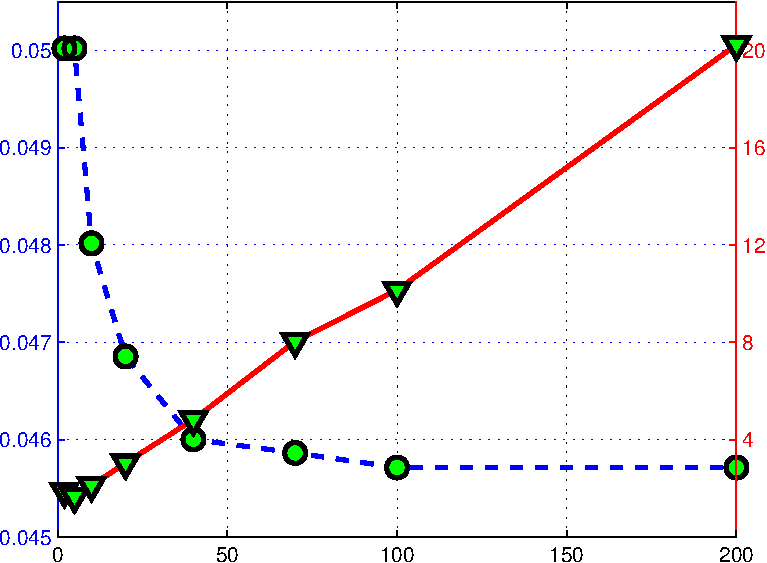
\includegraphics[width=0.9\linewidth]{figures/varyM}
		\label{fig:matlabgood}
	}
	\end{minipage}\hfill
	\begin{minipage}{0.4\linewidth}
	\centering
	\subfigure[Matlab plot saved in bitmap form. The quality is bad. Remember: Export your figures as vector graphic if possible.]{
		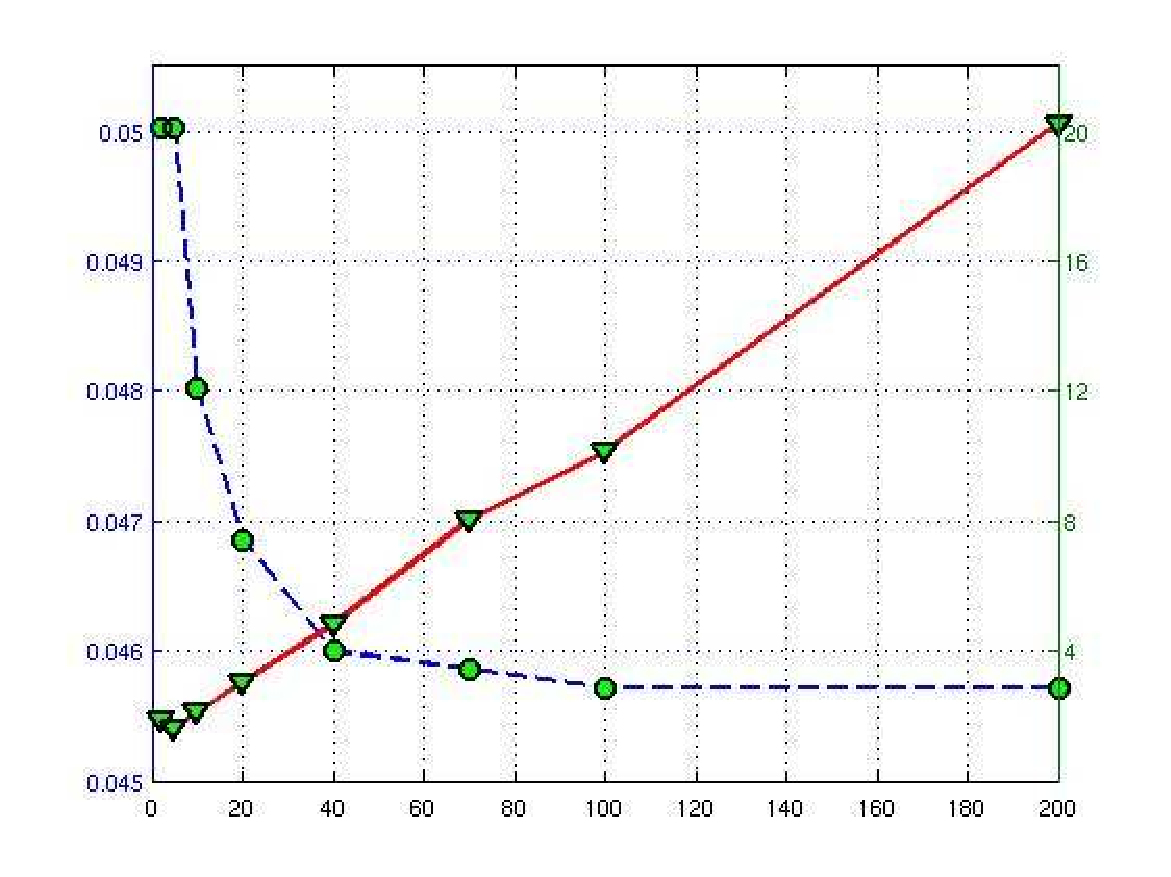
\includegraphics[width=0.9\linewidth]{figures/varyM_jpg}
		\label{fig:matlabbad}
	}
	\end{minipage}
\hfill
	\caption{Comparison of a vector and a rasterized plot.}
	\label{fig:matlabcomp}
\end{figure}


\paragraph*{How to draw high-quality graphics?}
Draw all your drawings with an application that supports vector graphics. My favorite is \textit{Inkscape}. Alternatives include Adobe Illustrator, sK1, yED, Xara Xtreme, OpenOffice Draw. Vector graphics can also directly drawn in latex using tikz notation or with help of TikzEdit.
These applications save your drawing automatically in vector form; if you include a photo it is usually still saved in bitmap form. \autoref{fig:nn} shows a graphic generated in tikz and \autoref{fig:faces} a graphic drawn with Inkscape. Even though a file saved as \textit{.eps} seems to be vectorized, it can also be completely rasterized. To check if your figure is still vectorized zoom in and verify that the text is still sharp. If not you figure might contain transparency or color gradients, which causes \textit{Inkscape} to raster the whole figure.

Make sure all graphics are \textit{well-readable} (line width, colors, fonts, arrows) and \textit{conclusive}. Also, all graphics in your thesis should be \textit{consistent} (same style). As you see in \autoref{fig:nn} and \autoref{fig:faces}, it is hard to create two figures of the same style by using two different tools.

\begin{figure}[H]
  \centering
  \resizebox{.65\textwidth}{!}{
\tikzset{neuron/.style={circle,thick,fill=black!25,minimum size=17pt,inner sep=0pt},
    hidden neuron/.style={neuron,draw,thick, fill=blue!30},
		output neuron/.style={neuron,draw,thick, fill=green!30},
    hoz/.style={rotate=90}}   %<--- for labels
    
    \def\layersep{2.5cm}
    
\begin{tikzpicture}
   \newcommand\Square[1]{+(-#1,-#1) rectangle +(#1,#1)}
   
%%%%%%%%%%%%%%
% Input layer
	\foreach \y / \lab in {1/n,3/j,5/2,6/1}{
	\draw  (0,\y) \Square{3pt} ;    
	\node (I-\y) at (0,\y) {};
	\node  at (-0.5,\y-0.05) {$x_\lab$};
	}

	% Draw dots
	\foreach \y in {2,4}
	\node[hoz]  at (0,\y) {$\dots$};

%%%%%%%%
% Hidden Layer 1
	\foreach \y  in {1,3,4,5}{
	\node[hidden neuron] (H1-\y) at (\layersep,0.5+\y) {};
	}
	% Draw dots
	\foreach \y in {2}
	\node[hoz]  at (\layersep,0.5+\y) {$\dots$};
	
	
	
%%%%%%%
% Connection I - H1
	\foreach \y  in {1,3,5,6}{
		\foreach \yy  in {1,3,4,5}{
		\draw [->, shorten >=0.5pt, thick]  (I-\y.center) -- (H1-\yy) ;
		}
	}
	
	% Draw Squares again
	\foreach \y / \lab in {1/n,3/k,5/2,6/1}
	\draw [fill=white] (0,\y) \Square{3pt} ;    
	

%%%%%%%%
% Hidden Layer 2
	\foreach \y  in {1,3,4}{
	\node[hidden neuron] (H2-\y) at (2*\layersep,1+\y) {};
	}
	% Draw dots
	\foreach \y in {2}
	\node[hoz]  at (2*\layersep,1+\y) {$\dots$};
	
	
	
%%%%%%%
% Connection H1 - H2
	\foreach \y  in {1,3,4,5}{
		\foreach \yy  in {1,3,4}{
		\draw [->, shorten >=0.5pt, thick]  (H1-\y) -- (H2-\yy) ;
		}
	}

	
		

%%%%%%%%
% Hidden Layer 3
	\foreach \y  in {1,3,4}{
	\node[hidden neuron] (H3-\y) at (3*\layersep,1+\y) {};
	}
	% Draw dots
	\foreach \y in {2}
	\node[hoz]  at (3*\layersep,1+\y) {$\dots$};
	
	
	
%%%%%%%
% Connection H2 - H3
	\foreach \y  in {1,3,4}{
		\foreach \yy  in {1,3,4}{
		\draw[-, thick]  (H2-\y) -- ($(H2-\y)!0.75cm!(H3-\yy)$);
		\draw[<-, thick]  (H3-\y) -- ($(H3-\y)!0.75cm!(H2-\yy)$);
		}
	}
	
	% Dots
	% Draw dots
	\foreach \y in {1,2,3,4}
	\node  at (2.5*\layersep,1+\y) {$\dots$};
	

	
	
	
	
	
%%%%%
% Output
	\node [output neuron] (O-1) at (4*\layersep,3.5){};
	
	% Connection
		\foreach \y  in {1,3,4}{
		\draw [->, shorten >=0.5pt, thick]  (H3-\y) -- (O-1) ;
		}
		
		
%%%%%
% Output
	\draw (12.5,3.5) \Square{3pt} ;    
	\node  (OO-1) at  (12.5,3.5) {};
	\node at (13,3.5){$y$};
	\draw [->, shorten >=-0.5pt, thick]  (O-1) -- (OO-1) ;

%%%%%%%%%
% Annotations

	\draw [dashed] (0 * \layersep-25,-0.25) rectangle (0 * \layersep+15,7);
	\draw [dashed] (5 * \layersep-15,-0.25) rectangle (5 * \layersep+25,7);
	\node at (0 * \layersep-5,0) {Inputs};
	\node at (5 * \layersep+5,0) {Output};

\end{tikzpicture}}
  \caption{Multilayer feedforward neural network generated with Tikz.}
  \label{fig:nn}
\end{figure}

\begin{figure}[H]
  \centering
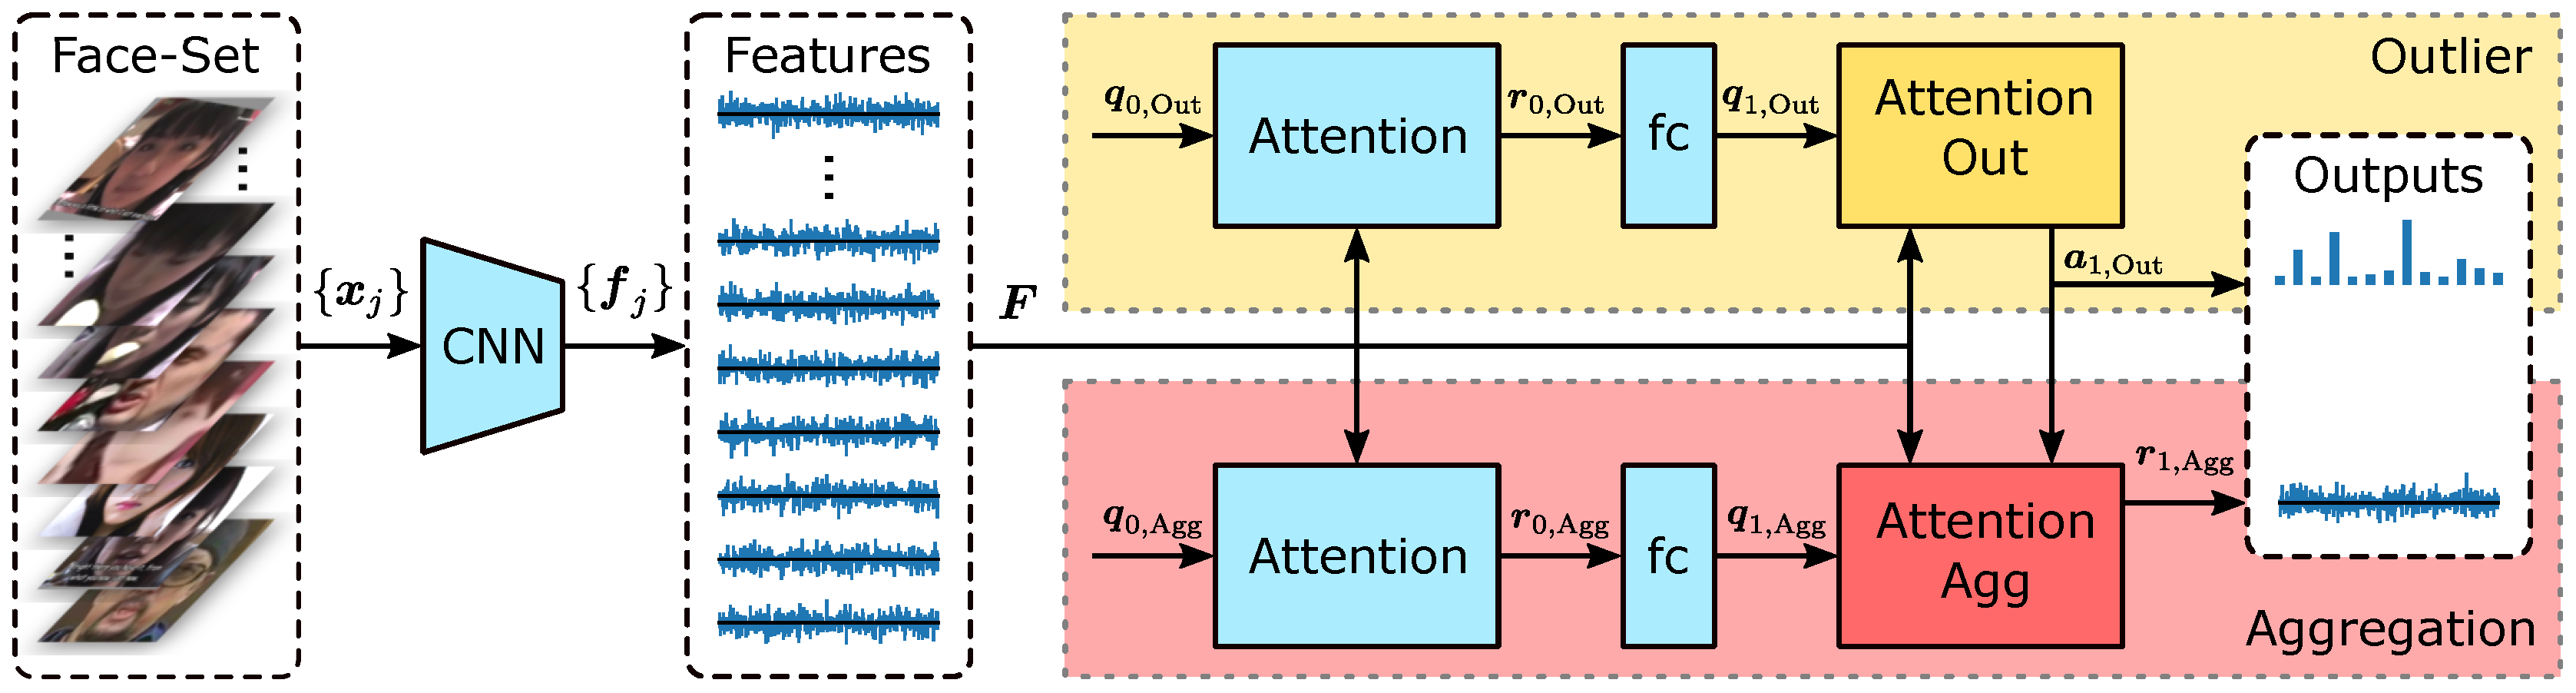
\includegraphics[width=0.87\linewidth]{figures/network.eps}
  \caption{Neural network architecture generated in Inkscape as shown in \cite{hoerman2019ORNAN}.}
  \label{fig:faces}
\end{figure}

\paragraph*{How to generate high-quality plots?}
Python plots (with \textit{matplotlib}) can be converted to tikz code and included in \LaTeX using the package \textit{matplotlib2tikz}.  The huge advantage is that all plots can be edited (labels, limits, ticks, legends, etc.) afterwards within latex without exporting it again. In  \autoref{fig:plot}, you can e.g. adjust the height of the figure by adjusting \verb'\setlength\figureheight{4cm}'. The plot will be generated again with the new height without deforming the text. For MATLAB you can use the script \textit{matlab2tikz}. Do not forget to \textit{label all axes} of your plots and include a \textit{legend}.

\begin{figure}[H]
  \centering
  \newlength\figureheight
\newlength\figurewidth
\setlength\figureheight{4cm}
\setlength\figurewidth{0.7\linewidth}
% This file was created by matplotlib2tikz v0.6.18.

\pgfplotsset{every tick label/.append style={font=\scriptsize}}
\begin{tikzpicture}

\definecolor{color4}{rgb}{0.580392156862745,0.403921568627451,0.741176470588235}
\definecolor{color5}{rgb}{0.549019607843137,0.337254901960784,0.294117647058824}
\definecolor{color2}{rgb}{0.172549019607843,0.627450980392157,0.172549019607843}
\definecolor{color6}{rgb}{0.890196078431372,0.466666666666667,0.76078431372549}
\definecolor{color0}{rgb}{0.12156862745098,0.466666666666667,0.705882352941177}
\definecolor{color1}{rgb}{1,0.498039215686275,0.0549019607843137}
\definecolor{color3}{rgb}{0.83921568627451,0.152941176470588,0.156862745098039}

\begin{groupplot}[group style={group size=2 by 2, vertical sep=50pt,horizontal sep=30pt}, title style={yshift=-1.5ex}]
\nextgroupplot[
height=\figureheight,
tick align=outside,
tick pos=left,
ylabel near ticks,
title={CMC},
width=0.5\figurewidth,
x grid style={white!69.01960784313725!black},
xlabel={Rank},
xmajorgrids,
xminorgrids,
xmin=1, xmax=100,
minor x tick num=10,
xmode=log,
ytick={0.75,0.8,0.85,0.9,0.95,1},
y grid style={white!69.01960784313725!black},
ylabel={TPIR},
ymajorgrids,
ymin=0.75, ymax=1,
every major tick/.style={black, semithick},
yminorgrids,
mark repeat={100}
]
\addplot [thick, color0, dashed, forget plot, mark=pentagon, mark options={solid}]
table [row sep=\\]{%
1	0.886687931404806 \\
2	0.910393874613219 \\
3	0.923837363625459 \\
4	0.930004181108705 \\
5	0.935157965559211 \\
6	0.939029638870805 \\
7	0.942337816075196 \\
8	0.944634278567514 \\
9	0.947085859984341 \\
10	0.94922720355215 \\
11	0.951115288861774 \\
12	0.952544609001202 \\
13	0.954076023436302 \\
14	0.955350224651221 \\
15	0.956577992840633 \\
16	0.957496841501693 \\
17	0.958468714791589 \\
18	0.959081280565629 \\
19	0.959801213918006 \\
20	0.960877818144907 \\
21	0.961744960497798 \\
22	0.962305819963668 \\
23	0.963020480033382 \\
24	0.963324126279071 \\
25	0.964345069235804 \\
26	0.964958953330511 \\
27	0.965367330513204 \\
28	0.965824777362735 \\
29	0.966026329312751 \\
30	0.966383000187274 \\
31	0.966893471665641 \\
32	0.967301848848335 \\
33	0.967507355760347 \\
34	0.967862708314206 \\
35	0.968170309521891 \\
36	0.96837713475457 \\
37	0.968784193616598 \\
38	0.969093113144949 \\
39	0.969349008044466 \\
40	0.96970567891899 \\
41	0.970008006844012 \\
42	0.970312971410367 \\
43	0.970667005643559 \\
44	0.970920263901744 \\
45	0.970971970209913 \\
46	0.97117615880126 \\
47	0.97143073538011 \\
48	0.971581899342622 \\
49	0.972088415858991 \\
50	0.972292604450338 \\
51	0.972600205658024 \\
52	0.972804394249371 \\
53	0.973007264520052 \\
54	0.973110677136391 \\
55	0.973263159419568 \\
56	0.973415641702745 \\
57	0.973619830294092 \\
58	0.973821382244107 \\
59	0.97397518284795 \\
60	0.974282784055636 \\
61	0.974334490363805 \\
62	0.974538678955152 \\
63	0.974640773250826 \\
64	0.974742867546499 \\
65	0.975049150433519 \\
66	0.97530372701237 \\
67	0.975404502987377 \\
68	0.975454890974881 \\
69	0.975505278962385 \\
70	0.975607373258058 \\
71	0.975761173861901 \\
72	0.975912337824412 \\
73	0.975962725811916 \\
74	0.97606482010759 \\
75	0.976217302390767 \\
76	0.976269008698936 \\
77	0.976320715007106 \\
78	0.976372421315276 \\
79	0.976575291585956 \\
80	0.976729092189799 \\
81	0.976829868164807 \\
82	0.976984987089316 \\
83	0.977240881988832 \\
84	0.977240881988832 \\
85	0.977344294605171 \\
86	0.977498095209014 \\
87	0.977651895812857 \\
88	0.977753990108531 \\
89	0.977854766083538 \\
90	0.977905154071042 \\
91	0.978109342662389 \\
92	0.978159730649892 \\
93	0.978363919241239 \\
94	0.978466013536913 \\
95	0.978621132461421 \\
96	0.978723226757095 \\
97	0.978825321052768 \\
98	0.978825321052768 \\
99	0.978927415348442 \\
100	0.979029509644115 \\
};
\addplot [thick, color1, forget plot, mark=x]
table [row sep=\\]{%
1	0.254023056125757 \\
2	0.477712533352731 \\
3	0.624988460786109 \\
4	0.740492995652877 \\
5	0.829493589783004 \\
6	0.879239586387052 \\
7	0.902287557314382 \\
8	0.91239357426538 \\
9	0.918269928709595 \\
10	0.922219674742675 \\
11	0.925595378103225 \\
12	0.928503088048918 \\
13	0.930845983566742 \\
14	0.932935620826382 \\
15	0.934773318148503 \\
16	0.936348528967778 \\
17	0.938176998045238 \\
18	0.939498950606328 \\
19	0.940879201078918 \\
20	0.942411933834684 \\
21	0.943484583099588 \\
22	0.944806535660678 \\
23	0.945677632975567 \\
24	0.946652142906794 \\
25	0.947877274454874 \\
26	0.948489840228915 \\
27	0.949254888286132 \\
28	0.950015981381352 \\
29	0.951088630646255 \\
30	0.95164817179146 \\
31	0.952210349577997 \\
32	0.95307353696889 \\
33	0.953891609654943 \\
34	0.95465665771216 \\
35	0.955316974832373 \\
36	0.956186753826595 \\
37	0.956743658330468 \\
38	0.957047304576157 \\
39	0.957511343029017 \\
40	0.958174296790561 \\
41	0.958682131627597 \\
42	0.959237717810804 \\
43	0.959695164660335 \\
44	0.960149974868535 \\
45	0.960812928630079 \\
46	0.961169599504603 \\
47	0.961530225341125 \\
48	0.961839144869476 \\
49	0.962148064397828 \\
50	0.962402640976679 \\
51	0.962757993530537 \\
52	0.963267146688238 \\
53	0.963521723267088 \\
54	0.963675523870931 \\
55	0.96392746380845 \\
56	0.964284134682974 \\
57	0.964691193545002 \\
58	0.964793287840675 \\
59	0.965099570727695 \\
60	0.965458878243551 \\
61	0.965814230797409 \\
62	0.966070125696925 \\
63	0.966324702275776 \\
64	0.966630985162796 \\
65	0.966835173754143 \\
66	0.967087113691662 \\
67	0.967341690270512 \\
68	0.967545878861859 \\
69	0.967955574365218 \\
70	0.968108056648395 \\
71	0.968463409202253 \\
72	0.968923492693117 \\
73	0.969127681284463 \\
74	0.969538695108488 \\
75	0.969795908328671 \\
76	0.969951027253179 \\
77	0.970002733561349 \\
78	0.970104827857022 \\
79	0.970358086115207 \\
80	0.97081816960607 \\
81	0.97086987591424 \\
82	0.97112445249309 \\
83	0.971227865109429 \\
84	0.971531511355118 \\
85	0.971733063305133 \\
86	0.971935933575814 \\
87	0.971935933575814 \\
88	0.972036709550822 \\
89	0.972138803846495 \\
90	0.972443768412849 \\
91	0.972544544387857 \\
92	0.97264663868353 \\
93	0.972800439287373 \\
94	0.972901215262381 \\
95	0.973157110161897 \\
96	0.973207498149401 \\
97	0.973257886136905 \\
98	0.973309592445074 \\
99	0.973463393048917 \\
100	0.973566805665256 \\
};
\addplot [thick, color2, forget plot, mark=+]
table [row sep=\\]{%
1	0.798470992933072 \\
2	0.859851341367829 \\
3	0.885433504999874 \\
4	0.897350852859677 \\
5	0.906937170087648 \\
6	0.912499331720848 \\
7	0.917495360605515 \\
8	0.920859199080073 \\
9	0.924528002120985 \\
10	0.927129429179657 \\
11	0.930287760742203 \\
12	0.933355862895068 \\
13	0.936203956608596 \\
14	0.938138474943726 \\
15	0.940128654549024 \\
16	0.94160704435529 \\
17	0.94344474167741 \\
18	0.944765375917835 \\
19	0.946042213774085 \\
20	0.94757230988852 \\
21	0.948794804795269 \\
22	0.949868772380838 \\
23	0.951042197620749 \\
24	0.952064458898149 \\
25	0.953548121987077 \\
26	0.954364876352464 \\
27	0.955125969447684 \\
28	0.955735898580393 \\
29	0.956702498587625 \\
30	0.957110875770319 \\
31	0.957923675173708 \\
32	0.958332052356402 \\
33	0.959046712426115 \\
34	0.959350358671804 \\
35	0.959859511829505 \\
36	0.960217501024695 \\
37	0.960575490219884 \\
38	0.961136349685755 \\
39	0.961848373114137 \\
40	0.962358844592504 \\
41	0.962822883045364 \\
42	0.963127847611719 \\
43	0.96358529446125 \\
44	0.96389157734827 \\
45	0.964295999568966 \\
46	0.964703058430994 \\
47	0.965006704676683 \\
48	0.965314305884369 \\
49	0.96572663802906 \\
50	0.966133696891087 \\
51	0.966337885482434 \\
52	0.966592462061284 \\
53	0.966897426627639 \\
54	0.967203709514659 \\
55	0.967763250659864 \\
56	0.968069533546884 \\
57	0.968272403817565 \\
58	0.968322791805069 \\
59	0.968529617037747 \\
60	0.968835899924767 \\
61	0.969189934157959 \\
62	0.969395441069972 \\
63	0.969757385227159 \\
64	0.970111419460352 \\
65	0.970315608051698 \\
66	0.970315608051698 \\
67	0.970518478322379 \\
68	0.970673597246888 \\
69	0.970826079530065 \\
70	0.971028949800746 \\
71	0.971282208058931 \\
72	0.971636242292123 \\
73	0.971892137191639 \\
74	0.971992913166647 \\
75	0.972096325782986 \\
76	0.972405245311338 \\
77	0.972507339607011 \\
78	0.972761916185862 \\
79	0.972964786456543 \\
80	0.973118587060386 \\
81	0.973168975047889 \\
82	0.973321457331067 \\
83	0.973577352230583 \\
84	0.97372983451376 \\
85	0.97403611740078 \\
86	0.9743424002878 \\
87	0.97444581290414 \\
88	0.974496200891643 \\
89	0.974496200891643 \\
90	0.974598295187317 \\
91	0.97464868317482 \\
92	0.974749459149828 \\
93	0.974799847137332 \\
94	0.974952329420509 \\
95	0.97515519969119 \\
96	0.975309000295033 \\
97	0.975462800898876 \\
98	0.975615283182053 \\
99	0.975769083785896 \\
100	0.975872496402235 \\
};
\addplot [thick, color3, forget plot, mark=diamond]
table [row sep=\\]{%
1	0.82894709115411 \\
2	0.867659577505844 \\
3	0.885416075029016 \\
4	0.895348516566184 \\
5	0.903350394730219 \\
6	0.909209611005779 \\
7	0.914108818877435 \\
8	0.919151280787607 \\
9	0.922914268200198 \\
10	0.92587368445406 \\
11	0.928939149965593 \\
12	0.931537940382934 \\
13	0.934085024492105 \\
14	0.935757056324391 \\
15	0.937789713993197 \\
16	0.939016163861944 \\
17	0.941409447367272 \\
18	0.942480778311509 \\
19	0.943603815563917 \\
20	0.944374136903797 \\
21	0.945601905093209 \\
22	0.946671917716781 \\
23	0.947435647453333 \\
24	0.948613027655241 \\
25	0.949685676920144 \\
26	0.950803440889888 \\
27	0.952275239092824 \\
28	0.953038968829376 \\
29	0.953854404874097 \\
30	0.954766661931829 \\
31	0.95553039166838 \\
32	0.956092569454917 \\
33	0.956600404291952 \\
34	0.957214288386658 \\
35	0.95741979529867 \\
36	0.957981973085207 \\
37	0.95874833946309 \\
38	0.959204467991956 \\
39	0.959661914841487 \\
40	0.960068973703515 \\
41	0.960373938269869 \\
42	0.960938752697737 \\
43	0.961295423572261 \\
44	0.961748915459795 \\
45	0.961901397742972 \\
46	0.96236016291317 \\
47	0.962718152108359 \\
48	0.963023116674714 \\
49	0.96322730526606 \\
50	0.963684752115592 \\
51	0.963888940706939 \\
52	0.964094447618951 \\
53	0.964297317889632 \\
54	0.96439809386464 \\
55	0.964856859034837 \\
56	0.965061047626184 \\
57	0.965163141921857 \\
58	0.965468106488212 \\
59	0.96562322541272 \\
60	0.965879120312237 \\
61	0.966083308903583 \\
62	0.966337885482434 \\
63	0.966542074073781 \\
64	0.966847038640135 \\
65	0.967101615218986 \\
66	0.96740657978534 \\
67	0.96771286267236 \\
68	0.967917051263707 \\
69	0.968224652471393 \\
70	0.968275040458896 \\
71	0.968326746767066 \\
72	0.968427522742074 \\
73	0.968580005025251 \\
74	0.968835899924767 \\
75	0.969139546170456 \\
76	0.96944451073681 \\
77	0.96975079362383 \\
78	0.969802499932 \\
79	0.969852887919503 \\
80	0.97010878281902 \\
81	0.970514523360382 \\
82	0.970668323964225 \\
83	0.970819487926736 \\
84	0.971076701146918 \\
85	0.971279571417599 \\
86	0.971380347392607 \\
87	0.971636242292123 \\
88	0.971686630279627 \\
89	0.97184043088347 \\
90	0.971941206858477 \\
91	0.972145395449824 \\
92	0.972399972028675 \\
93	0.972605478940687 \\
94	0.972657185248857 \\
95	0.972809667532034 \\
96	0.972913080148373 \\
97	0.973016492764712 \\
98	0.973168975047889 \\
99	0.973426188268072 \\
100	0.97358130719258 \\
};
\addplot [thick, color0, forget plot, mark=pentagon]
table [row sep=\\]{%
1	0.709391007760792 \\
2	0.778013167782827 \\
3	0.799781956014778 \\
4	0.812029316533586 \\
5	0.821054774295686 \\
6	0.82768299359046 \\
7	0.833341976236671 \\
8	0.837590095232775 \\
9	0.841932398600558 \\
10	0.846314543390519 \\
11	0.850186216702112 \\
12	0.853292841956488 \\
13	0.855688762103148 \\
14	0.857777081042121 \\
15	0.859620051646906 \\
16	0.861966902126727 \\
17	0.863801962807517 \\
18	0.865231282946944 \\
19	0.866866109998384 \\
20	0.868703807320504 \\
21	0.870335997730613 \\
22	0.871717566523868 \\
23	0.87340014492148 \\
24	0.874678301098396 \\
25	0.875947229030651 \\
26	0.876974763590714 \\
27	0.8782463281643 \\
28	0.879215564812865 \\
29	0.880184801461429 \\
30	0.881409933009509 \\
31	0.882733203891266 \\
32	0.883601664564822 \\
33	0.884525786508546 \\
34	0.885190058590756 \\
35	0.885907355301801 \\
36	0.886518602755175 \\
37	0.887027755912877 \\
38	0.887845828598929 \\
39	0.888710334310489 \\
40	0.889727322305225 \\
41	0.890288181771095 \\
42	0.890948498891308 \\
43	0.891763934936029 \\
44	0.892121924131219 \\
45	0.892783559572097 \\
46	0.893241006421629 \\
47	0.894263267699028 \\
48	0.894822808844233 \\
49	0.895280255693764 \\
50	0.895992279122146 \\
51	0.896858103154371 \\
52	0.897316868324569 \\
53	0.897928115777943 \\
54	0.898441223897642 \\
55	0.898797894772166 \\
56	0.89935743591737 \\
57	0.899612012496221 \\
58	0.900276284578431 \\
59	0.900944511622638 \\
60	0.901606147063516 \\
61	0.902015842566876 \\
62	0.902523677403911 \\
63	0.902982442574108 \\
64	0.903389501436136 \\
65	0.904049818556348 \\
66	0.904407807751538 \\
67	0.905121149500586 \\
68	0.905375726079436 \\
69	0.905682008966456 \\
70	0.906036043199649 \\
71	0.906496126690512 \\
72	0.90710605582322 \\
73	0.90746404501841 \\
74	0.907766372943433 \\
75	0.90817343180546 \\
76	0.90853142100065 \\
77	0.908890728516506 \\
78	0.909246081070364 \\
79	0.910062835435751 \\
80	0.910419506310275 \\
81	0.910776177184799 \\
82	0.911033390404981 \\
83	0.911289285304497 \\
84	0.911956194028039 \\
85	0.912414959198236 \\
86	0.912926748997269 \\
87	0.913133574229947 \\
88	0.913438538796301 \\
89	0.913895985645833 \\
90	0.914153198866015 \\
91	0.914561576048708 \\
92	0.914867858935729 \\
93	0.915326624105926 \\
94	0.915735001288619 \\
95	0.915941826521298 \\
96	0.916146015112644 \\
97	0.916452297999665 \\
98	0.916604780282842 \\
99	0.916706874578515 \\
100	0.917015794106867 \\
};
\addplot [thick, color4, forget plot, mark=o]
table [row sep=\\]{%
1	0.846311031342579 \\
2	0.885611035375702 \\
3	0.900369593543501 \\
4	0.908934967814738 \\
5	0.915038214103822 \\
6	0.920283546284675 \\
7	0.923860801595241 \\
8	0.927626425649164 \\
9	0.930632274928532 \\
10	0.933642079169898 \\
11	0.935526209517525 \\
12	0.936951574694955 \\
13	0.938382213155048 \\
14	0.939602071420465 \\
15	0.940974411969059 \\
16	0.94265435372534 \\
17	0.943675296682074 \\
18	0.944546393996962 \\
19	0.945567336953695 \\
20	0.946431842665255 \\
21	0.947499218647495 \\
22	0.94836504267972 \\
23	0.949383348995122 \\
24	0.949991959807165 \\
25	0.951114997059572 \\
26	0.95182833880862 \\
27	0.952794938815852 \\
28	0.953200679357214 \\
29	0.953920612709591 \\
30	0.954632636137973 \\
31	0.954887212716823 \\
32	0.955547529837036 \\
33	0.956462423536099 \\
34	0.956817776089957 \\
35	0.95727785958082 \\
36	0.957736624751017 \\
37	0.958449966500065 \\
38	0.958959119657766 \\
39	0.959163308249113 \\
40	0.959624710060642 \\
41	0.959777192343819 \\
42	0.960131226577011 \\
43	0.960387121476527 \\
44	0.960641698055378 \\
45	0.961050075238072 \\
46	0.961410701074593 \\
47	0.961612253024608 \\
48	0.961866829603458 \\
49	0.961917217590962 \\
50	0.962069699874139 \\
51	0.962273888465486 \\
52	0.962629241019344 \\
53	0.962984593573202 \\
54	0.963289558139557 \\
55	0.963392970755896 \\
56	0.963646229014081 \\
57	0.963798711297258 \\
58	0.964054606196774 \\
59	0.964156700492448 \\
60	0.964409958750632 \\
61	0.964614147341979 \\
62	0.964867405600164 \\
63	0.965070275870845 \\
64	0.965221439833356 \\
65	0.965478653053538 \\
66	0.965835323928062 \\
67	0.965835323928062 \\
68	0.965937418223735 \\
69	0.966088582186247 \\
70	0.96619067648192 \\
71	0.966445253060771 \\
72	0.966597735343948 \\
73	0.966750217627125 \\
74	0.966852311922798 \\
75	0.967057818834811 \\
76	0.967264644067489 \\
77	0.967315032054993 \\
78	0.967365420042497 \\
79	0.967517902325674 \\
80	0.967720772596355 \\
81	0.967874573200198 \\
82	0.967976667495871 \\
83	0.968129149779048 \\
84	0.968232562395388 \\
85	0.968282950382891 \\
86	0.96848977561557 \\
87	0.968692645886251 \\
88	0.968996292131939 \\
89	0.969303893339625 \\
90	0.969355599647795 \\
91	0.969508081930972 \\
92	0.969710952201653 \\
93	0.970017235088673 \\
94	0.970068941396843 \\
95	0.970119329384346 \\
96	0.970273129988189 \\
97	0.970375224283863 \\
98	0.970426930592032 \\
99	0.970578094554544 \\
100	0.970628482542047 \\
};
\addplot [thick, color5, forget plot, mark=triangle]
table [row sep=\\]{%
1	0.857988304150855 \\
2	0.89041605887568 \\
3	0.904393749138272 \\
4	0.913148810473531 \\
5	0.919269194931271 \\
6	0.924255995571276 \\
7	0.928331857474216 \\
8	0.931901202860787 \\
9	0.934656430523302 \\
10	0.936842888795952 \\
11	0.93822050262721 \\
12	0.939442997533959 \\
13	0.940865726070057 \\
14	0.942706060033509 \\
15	0.943723048028246 \\
16	0.94494686125566 \\
17	0.946120286495571 \\
18	0.946934404219627 \\
19	0.947798909931186 \\
20	0.948668688925408 \\
21	0.949640562215304 \\
22	0.950457316580691 \\
23	0.951624150217273 \\
24	0.952540362237001 \\
25	0.953302773652887 \\
26	0.953864951439424 \\
27	0.954472243930801 \\
28	0.955184267359183 \\
29	0.955540938233707 \\
30	0.956202573674585 \\
31	0.95676211481979 \\
32	0.957065761065478 \\
33	0.957677008518853 \\
34	0.958236549664057 \\
35	0.958542832551078 \\
36	0.958902140066933 \\
37	0.959413929865966 \\
38	0.959974789331836 \\
39	0.96007688362751 \\
40	0.960430917860702 \\
41	0.960735882427056 \\
42	0.960990459005907 \\
43	0.961296741892927 \\
44	0.961499612163608 \\
45	0.961804576729962 \\
46	0.962159929283821 \\
47	0.962260705258828 \\
48	0.962616057812686 \\
49	0.962922340699706 \\
50	0.963329399561734 \\
51	0.963481881844911 \\
52	0.963992353323278 \\
53	0.964195223593959 \\
54	0.964606237417984 \\
55	0.964761356342493 \\
56	0.964964226613174 \\
57	0.965067639229513 \\
58	0.96527182782086 \\
59	0.965627180374718 \\
60	0.965678886682887 \\
61	0.965985169569908 \\
62	0.966136333532419 \\
63	0.966340522123766 \\
64	0.966544710715112 \\
65	0.966595098702616 \\
66	0.966799287293963 \\
67	0.96700347588531 \\
68	0.967155958168487 \\
69	0.967360146759834 \\
70	0.967462241055507 \\
71	0.967565653671846 \\
72	0.967769842263193 \\
73	0.967821548571362 \\
74	0.967923642867036 \\
75	0.968278995420894 \\
76	0.968533571999744 \\
77	0.96884117320743 \\
78	0.969044043478111 \\
79	0.969245595428126 \\
80	0.9693476897238 \\
81	0.969603584623316 \\
82	0.969704360598324 \\
83	0.969754748585828 \\
84	0.96990854918967 \\
85	0.970009325164678 \\
86	0.970110101139686 \\
87	0.970365996039202 \\
88	0.970673597246888 \\
89	0.970824761209399 \\
90	0.970975925171911 \\
91	0.971127089134422 \\
92	0.971280889738265 \\
93	0.971434690342108 \\
94	0.971536784637781 \\
95	0.971690585241624 \\
96	0.971792679537298 \\
97	0.971947798461806 \\
98	0.972048574436814 \\
99	0.972254081348827 \\
100	0.97230446933633 \\
};
\addplot [thick, color6, forget plot, mark=oplus]
table [row sep=\\]{%
1	0.863435188281724 \\
2	0.893510819244064 \\
3	0.906520591178757 \\
4	0.914875185255318 \\
5	0.919721368498139 \\
6	0.924661736112638 \\
7	0.928380927141054 \\
8	0.932057640105962 \\
9	0.935166902001669 \\
10	0.937508479198828 \\
11	0.939187102634442 \\
12	0.940051608346002 \\
13	0.941071232982069 \\
14	0.942858542316686 \\
15	0.944233519506612 \\
16	0.945357875079685 \\
17	0.9465816883071 \\
18	0.947391851069158 \\
19	0.948152944164378 \\
20	0.949173887121112 \\
21	0.949895138794155 \\
22	0.950662823492703 \\
23	0.951681129808106 \\
24	0.952645093174006 \\
25	0.953357116602389 \\
26	0.954071776672102 \\
27	0.954627362855309 \\
28	0.955599236145205 \\
29	0.95590420071156 \\
30	0.956515448164934 \\
31	0.957076307630805 \\
32	0.957178401926478 \\
33	0.957940813342364 \\
34	0.958297484216888 \\
35	0.958655473412078 \\
36	0.959063850594771 \\
37	0.959421839789961 \\
38	0.959726804356315 \\
39	0.960030450602004 \\
40	0.960384484835196 \\
41	0.960688131080884 \\
42	0.96099573228857 \\
43	0.961148214571747 \\
44	0.96130201517559 \\
45	0.961454497458768 \\
46	0.961707755716952 \\
47	0.96180853169196 \\
48	0.962163884245818 \\
49	0.962264660220825 \\
50	0.962825519686696 \\
51	0.9628759076742 \\
52	0.963232578548724 \\
53	0.963435448819405 \\
54	0.963845144322764 \\
55	0.964102357542946 \\
56	0.964356934121797 \\
57	0.964562441033809 \\
58	0.964763992983825 \\
59	0.964915156946336 \\
60	0.965018569562675 \\
61	0.965323534129029 \\
62	0.96552640439971 \\
63	0.965677568362222 \\
64	0.965933463261738 \\
65	0.966036875878077 \\
66	0.966188039840588 \\
67	0.966392228431935 \\
68	0.966442616419439 \\
69	0.966646805010786 \\
70	0.966801923935295 \\
71	0.967057818834811 \\
72	0.967413171388669 \\
73	0.967515265684342 \\
74	0.967669066288185 \\
75	0.96792232454637 \\
76	0.968176901125221 \\
77	0.96822860743339 \\
78	0.968434114345403 \\
79	0.968636984616084 \\
80	0.968688690924253 \\
81	0.96884117320743 \\
82	0.968994973811273 \\
83	0.969097068106947 \\
84	0.969249550390124 \\
85	0.969350326365132 \\
86	0.969502808648309 \\
87	0.96970567891899 \\
88	0.969961573818506 \\
89	0.970062349793513 \\
90	0.970265220064194 \\
91	0.970466772014209 \\
92	0.970670960605556 \\
93	0.970722666913726 \\
94	0.970774373221895 \\
95	0.970928173825738 \\
96	0.971081974429581 \\
97	0.971235775033424 \\
98	0.971386938995936 \\
99	0.971540739599779 \\
100	0.971591127587282 \\
};
\nextgroupplot[
height=\figureheight,
legend cell align={left},
legend entries={{optimal},{Baseline 1},{Baseline 2},{Baseline 3},{Baseline 4},{Baseline 5},{Ours 1},{Ours 2}},
legend columns=4, 
legend style={
at={(-0.2,-0.7)}, 
anchor=center, 
font=\scriptsize,
/tikz/every even column/.append style={column sep=0.2cm},
draw=white!80.0!black},
tick align=outside,
tick pos=left,
title={IET},
width=0.5\figurewidth,
x grid style={lightgray!92.02614379084967!black},
xlabel={FPIR},
xmajorgrids,
xmin=0.001, xmax=1,
xminorgrids,
xmode=log,
y grid style={lightgray!92.02614379084967!black},
%ylabel={TPIR},
ytick={0.01,0.1,1},
yticklabels={0.01,0.1,1},
ymajorgrids,
every major tick/.style={black, semithick},
ymin=0.01, ymax=1,
yminorgrids,
ymode=log,
mark repeat={100}
]
\addlegendimage{color0, thick, dashed, mark=pentagon, mark options={solid}}
\addlegendimage{color1, thick, mark=x}
\addlegendimage{color2, thick, mark=+}
\addlegendimage{color3, thick, mark=diamond}
\addlegendimage{color0, thick, mark=pentagon}
\addlegendimage{color4, thick, mark=o}
\addlegendimage{color5, thick, mark=triangle}
\addlegendimage{color6, thick, mark=oplus}
\addplot [thick, color0, dashed, mark=pentagon, mark options={solid}]
table [row sep=\\]{%
0	0 \\
0	0 \\
0	0 \\
0	0 \\
0	0 \\
0	0.000102094295673316 \\
0	0.000204188591346743 \\
0	0.000509153157701059 \\
0	0.00101698799473626 \\
0	0.00132458920242229 \\
0	0.00167994175628039 \\
0	0.0026929747890192 \\
0	0.00370732614242386 \\
0	0.00477338380399817 \\
0	0.00685642946030862 \\
0	0.0096554535069987 \\
0	0.0130206103022227 \\
0	0.017360277028674 \\
0	0.0219969983974848 \\
0	0.0292338285043021 \\
0	0.0379424568140556 \\
0	0.0497788035088381 \\
0	0.0640865064304348 \\
0	0.080107109124957 \\
0	0.0990818547906783 \\
0	0.119142724730164 \\
0	0.146271830843097 \\
5.03879875037791e-05	0.176483832438421 \\
5.03879875037791e-05	0.207871604112785 \\
0.000151163962511337	0.242510573400708 \\
0.000151163962511337	0.277933047235169 \\
0.000354034233192271	0.312780160076435 \\
0.000454810208199829	0.351151503599432 \\
0.000454810208199829	0.386615428978939 \\
0.000811481082723736	0.424480547787769 \\
0.000811481082723736	0.464173843871857 \\
0.000913575378397112	0.50475068576123 \\
0.00137102222792858	0.5413547865618 \\
0.00218645827264977	0.5790463299568 \\
0.00330290392172781	0.615511423483053 \\
0.0054468841308687	0.647303909180316 \\
0.0102242228968643	0.678889569644901 \\
0.0158380908382341	0.711264007938687 \\
0.0256803029657213	0.7392259800672 \\
0.0410830666035401	0.764164964747688 \\
0.0664818429726891	0.787069973438705 \\
0.104742890473815	0.809616992934531 \\
0.151489921204026	0.829986782402368 \\
0.219061259808071	0.846250388591951 \\
0.301423088078098	0.860822188139262 \\
0.402918001184092	0.875466787125395 \\
0.518623796198672	0.888565470149104 \\
0.635572152732191	0.902026097329999 \\
0.748844088103005	0.915794325718581 \\
0.844636805783019	0.926412132468612 \\
0.918683730286807	0.936108453916251 \\
0.963161540344625	0.944309247388969 \\
0.987927241413486	0.951030332734757 \\
0.996803145335943	0.956495673354947 \\
0.99969371711298	0.962089766486329 \\
0.999897905704327	0.965814230797409 \\
1	0.969066746731633 \\
1	0.970753280091242 \\
1	0.971930660293151 \\
1	0.972189191833999 \\
1	0.972292604450338 \\
1	0.972292604450338 \\
1	0.972292604450338 \\
1	0.972292604450338 \\
1	0.972292604450338 \\
1	0.972292604450338 \\
1	0.972292604450338 \\
1	0.972292604450338 \\
1	0.972292604450338 \\
1	0.972292604450338 \\
1	0.972292604450338 \\
1	0.972292604450338 \\
1	0.972292604450338 \\
1	0.972292604450338 \\
1	0.972292604450338 \\
1	0.972292604450338 \\
1	0.972292604450338 \\
1	0.972292604450338 \\
1	0.972292604450338 \\
1	0.972292604450338 \\
1	0.972292604450338 \\
1	0.972292604450338 \\
1	0.972292604450338 \\
1	0.972292604450338 \\
1	0.972292604450338 \\
1	0.972292604450338 \\
1	0.972292604450338 \\
1	0.972292604450338 \\
1	0.972292604450338 \\
1	0.972292604450338 \\
1	0.972292604450338 \\
1	0.972292604450338 \\
1	0.972292604450338 \\
1	0.972292604450338 \\
1	0.972292604450338 \\
};
\addplot [thick, color1, mark=x]
table [row sep=\\]{%
0	0 \\
0.689380525808811	0 \\
0.689380525808811	0.000201551950015144 \\
0.689380525808811	0.000664272082209871 \\
0.689380525808811	0.00182715075679418 \\
0.689380525808811	0.00442462285346912 \\
0.689380525808811	0.00990871176518349 \\
0.689380525808811	0.0168672355211655 \\
0.689380525808811	0.0233617208242871 \\
0.689380525808811	0.0284585256839609 \\
0.689380525808811	0.032737257857582 \\
0.689380525808811	0.0368595527860285 \\
0.689380525808811	0.0396704417187108 \\
0.689380525808811	0.0432160573332967 \\
0.689380525808811	0.047374238721923 \\
0.689380525808811	0.0507911018253165 \\
0.689380525808811	0.0554676646163046 \\
0.689380525808811	0.060552604589986 \\
0.689380525808811	0.0651906442794628 \\
0.689380525808811	0.0718850714097309 \\
0.689380525808811	0.0772776125910983 \\
0.68943223211698	0.0855011093173381 \\
0.68948393842515	0.0916455153492648 \\
0.68948393842515	0.100118023569489 \\
0.68948393842515	0.108729830866233 \\
0.68948393842515	0.120192076715633 \\
0.68948393842515	0.136125378444009 \\
0.68948393842515	0.154502351665216 \\
0.68948393842515	0.176183255326615 \\
0.68948393842515	0.203888014234945 \\
0.68948393842515	0.236357663418873 \\
0.68948393842515	0.270032669340895 \\
0.68948393842515	0.303822952765248 \\
0.689685490375165	0.345612185910101 \\
0.689787584670838	0.386384722862421 \\
0.690246349841036	0.425735849599309 \\
0.690348444136709	0.470265808879353 \\
0.690961009910749	0.513853189726353 \\
0.691369387093443	0.55460463354802 \\
0.692591882000192	0.596557479145782 \\
0.694681519259831	0.636868906088776 \\
0.698756062842105	0.674646432129257 \\
0.702438049089676	0.711320695727317 \\
0.709393644402124	0.746160190446792 \\
0.720214321422836	0.77697845801503 \\
0.735429008119501	0.802470392237394 \\
0.755765547768489	0.827160073621696 \\
0.779965850805077	0.849803914130532 \\
0.808823968341128	0.870856723972103 \\
0.843631531562421	0.88878547858844 \\
0.87886622025793	0.901803160447128 \\
0.912396945622972	0.914954868099673 \\
0.94376259764822	0.927609287480508 \\
0.969344761280265	0.937585525401851 \\
0.9850702112575	0.944959017943855 \\
0.993793341094577	0.949899385558355 \\
0.998225873872041	0.954179436052642 \\
0.999746741741815	0.957085827677668 \\
0.999949612012496	0.959488339427657 \\
1	0.961274330441608 \\
1	0.961836508228145 \\
1	0.962195815744 \\
1	0.962299228360339 \\
1	0.962402640976679 \\
1	0.962402640976679 \\
1	0.962402640976679 \\
1	0.962402640976679 \\
1	0.962402640976679 \\
1	0.962402640976679 \\
1	0.962402640976679 \\
1	0.962402640976679 \\
1	0.962402640976679 \\
1	0.962402640976679 \\
1	0.962402640976679 \\
1	0.962402640976679 \\
1	0.962402640976679 \\
1	0.962402640976679 \\
1	0.962402640976679 \\
1	0.962402640976679 \\
1	0.962402640976679 \\
1	0.962402640976679 \\
1	0.962402640976679 \\
1	0.962402640976679 \\
1	0.962402640976679 \\
1	0.962402640976679 \\
1	0.962402640976679 \\
1	0.962402640976679 \\
1	0.962402640976679 \\
1	0.962402640976679 \\
1	0.962402640976679 \\
1	0.962402640976679 \\
1	0.962402640976679 \\
1	0.962402640976679 \\
1	0.962402640976679 \\
1	0.962402640976679 \\
1	0.962402640976679 \\
1	0.962402640976679 \\
1	0.962402640976679 \\
1	0.962402640976679 \\
1	0.962402640976679 \\
};
\addplot [thick, color2, mark=+]
table [row sep=\\]{%
0	0 \\
0	0 \\
0	0 \\
0	0 \\
0	0 \\
0	5.17063081695301e-05 \\
0	0.000153800603842957 \\
0	0.000458765170197273 \\
0	0.000763729736551588 \\
0	0.00086714235289076 \\
0	0.000969236648564187 \\
0	0.00107133094423761 \\
0	0.00112303725240714 \\
0	0.00112303725240714 \\
0	0.00127551953558425 \\
0	0.00142800181876146 \\
0	0.00147838980626525 \\
0	0.00158180242260442 \\
0	0.00173428470578152 \\
0	0.00193847329712837 \\
0	0.00209227390097122 \\
0	0.00234421383849015 \\
0	0.00264786008417861 \\
0	0.00295150632986718 \\
0	0.00325778921688724 \\
0	0.00371655438708463 \\
0	0.00428136881495267 \\
0	0.00479315861398544 \\
0	0.00570409735105093 \\
0	0.0068709309876327 \\
0	0.00778450636602979 \\
0	0.0088028126814319 \\
0	0.0105384157078793 \\
0	0.0123721580680026 \\
0	0.0148276944468269 \\
0	0.0178892049963624 \\
0	0.0226543870741629 \\
5.03879875037791e-05	0.0271386261597966 \\
5.03879875037791e-05	0.0326145133453133 \\
5.03879875037791e-05	0.0396284065692596 \\
0.000151163962511337	0.0484124709591673 \\
0.000151163962511337	0.0611090766013089 \\
0.000251939937518895	0.0740816437551567 \\
0.000302327925022675	0.0911472109806002 \\
0.000710705107716178	0.11052242390502 \\
0.00101698799473631	0.133355659675676 \\
0.00194242825912578	0.160702137586614 \\
0.00316624148654047	0.191767806525969 \\
0.00582069317404824	0.226819107958582 \\
0.00985803197547694	0.266020389053624 \\
0.0162422212567275	0.309636772955272 \\
0.0262619637600423	0.356219456516313 \\
0.0434335802431567	0.408419962980722 \\
0.0672969872152076	0.460742630352994 \\
0.106897709050485	0.511679773970014 \\
0.161352199943703	0.565355007080893 \\
0.234369396160154	0.620035071498314 \\
0.323399285147132	0.673887834985021 \\
0.431230344386002	0.721970293285183 \\
0.552247387614726	0.768678066197622 \\
0.679917990033079	0.81064306848358 \\
0.797968582490555	0.851380302580125 \\
0.891746364274823	0.887888165972091 \\
0.954698260369061	0.917478957153119 \\
0.987666073231306	0.940032860054477 \\
0.99857463482257	0.954587521433132 \\
1	0.963078777944881 \\
1	0.965830050645399 \\
1	0.966133696891087 \\
1	0.966133696891087 \\
1	0.966133696891087 \\
1	0.966133696891087 \\
1	0.966133696891087 \\
1	0.966133696891087 \\
1	0.966133696891087 \\
1	0.966133696891087 \\
1	0.966133696891087 \\
1	0.966133696891087 \\
1	0.966133696891087 \\
1	0.966133696891087 \\
1	0.966133696891087 \\
1	0.966133696891087 \\
1	0.966133696891087 \\
1	0.966133696891087 \\
1	0.966133696891087 \\
1	0.966133696891087 \\
1	0.966133696891087 \\
1	0.966133696891087 \\
1	0.966133696891087 \\
1	0.966133696891087 \\
1	0.966133696891087 \\
1	0.966133696891087 \\
1	0.966133696891087 \\
1	0.966133696891087 \\
1	0.966133696891087 \\
1	0.966133696891087 \\
1	0.966133696891087 \\
1	0.966133696891087 \\
1	0.966133696891087 \\
1	0.966133696891087 \\
};
\addplot [thick, color3, mark=diamond]
table [row sep=\\]{%
0	0 \\
0	0 \\
0	0 \\
0	0 \\
0	0 \\
0	0.000102094295673316 \\
0	0.000204188591346743 \\
0	0.000509153157701059 \\
0	0.000763729736551588 \\
0	0.00086714235289076 \\
0	0.00107001262357176 \\
0	0.0012742012149185 \\
0	0.00137629551059182 \\
0	0.00157784746060696 \\
0	0.00228987088898891 \\
0	0.00280166068802168 \\
0	0.00361709673274291 \\
0	0.00494168593516509 \\
0	0.00706589133431867 \\
0	0.00996041807335302 \\
0	0.0129171976858835 \\
0	0.0171985665008362 \\
0	0.0225591761840214 \\
0	0.0298714423709929 \\
0	0.0393754401132776 \\
0	0.0516982367122396 \\
0	0.0692821853400449 \\
0	0.0881031304019231 \\
0	0.108903708503773 \\
0	0.13384503802339 \\
5.03879875037791e-05	0.162577039689581 \\
5.03879875037791e-05	0.193467814894439 \\
0.000100775975007558	0.225538315140335 \\
0.000151163962511337	0.262492203409896 \\
0.000151163962511337	0.298319099465054 \\
0.000251939937518895	0.335988966124995 \\
0.000605974170711167	0.374217347411678 \\
0.00126629129092357	0.412777351480234 \\
0.00203002102747516	0.449769762851308 \\
0.00341027150006446	0.485992144684703 \\
0.00550122708036993	0.522836320536799 \\
0.0100026043346592	0.563326596176286 \\
0.0164226800760895	0.599794326343872 \\
0.0274501823294799	0.634473428856174 \\
0.0462447609780418	0.66516294391322 \\
0.0705547764320949	0.696264791114956 \\
0.108427513362717	0.724511952999836 \\
0.163800852916996	0.752373149153341 \\
0.233240502020678	0.777158333229987 \\
0.319000736904777	0.799855198367659 \\
0.424840298217683	0.821623986599609 \\
0.540308654822068	0.842411673297003 \\
0.658949401602265	0.862244624873157 \\
0.777822021707791	0.879722816045494 \\
0.86897933633966	0.89646891717726 \\
0.935072134025585	0.910633657862543 \\
0.973875141589203	0.924002737313092 \\
0.991169210782383	0.93542147858052 \\
0.998224555551375	0.94494686125566 \\
0.999645965766808	0.951978184450465 \\
0.999949612012496	0.958440738255404 \\
1	0.961540771906451 \\
1	0.962968773725213 \\
1	0.963530951511749 \\
1	0.963684752115592 \\
1	0.963684752115592 \\
1	0.963684752115592 \\
1	0.963684752115592 \\
1	0.963684752115592 \\
1	0.963684752115592 \\
1	0.963684752115592 \\
1	0.963684752115592 \\
1	0.963684752115592 \\
1	0.963684752115592 \\
1	0.963684752115592 \\
1	0.963684752115592 \\
1	0.963684752115592 \\
1	0.963684752115592 \\
1	0.963684752115592 \\
1	0.963684752115592 \\
1	0.963684752115592 \\
1	0.963684752115592 \\
1	0.963684752115592 \\
1	0.963684752115592 \\
1	0.963684752115592 \\
1	0.963684752115592 \\
1	0.963684752115592 \\
1	0.963684752115592 \\
1	0.963684752115592 \\
1	0.963684752115592 \\
1	0.963684752115592 \\
1	0.963684752115592 \\
1	0.963684752115592 \\
1	0.963684752115592 \\
1	0.963684752115592 \\
1	0.963684752115592 \\
1	0.963684752115592 \\
1	0.963684752115592 \\
1	0.963684752115592 \\
1	0.963684752115592 \\
};
\addplot [thick, color0, mark=pentagon]
table [row sep=\\]{%
0	0 \\
0.000100775975007558	0 \\
0.000405740541361868	0 \\
0.000556904503873205	0 \\
0.000658998799546581	0 \\
0.00101435135340467	0.000102094295673316 \\
0.0014691615616045	0.000204188591346743 \\
0.0020260660654777	0.000509153157701059 \\
0.00253258258184713	0.00086450571155916 \\
0.00374980420593273	0.00117210691924508 \\
0.00481190690550955	0.00152745947310318 \\
0.00638843604545069	0.00208304565631057 \\
0.00811085586523991	0.00264258680151541 \\
0.0102403345470568	0.00330290392172783 \\
0.0123273351653648	0.00472299581649438 \\
0.0152775231745662	0.00640030093144306 \\
0.0176681700385627	0.00839179885740682 \\
0.0206687460352678	0.0110436139035829 \\
0.0237714163276464	0.0143557460699715 \\
0.0271273448782096	0.0184833142810812 \\
0.0305840494037804	0.0240296560662916 \\
0.0349503743457508	0.0318339372423087 \\
0.0382625065121393	0.04026528571969 \\
0.0423782098372567	0.050891002393716 \\
0.0472191197974142	0.0625429353071391 \\
0.0523412645519414	0.0760789985681891 \\
0.0568653450597522	0.0955325760162975 \\
0.0619993547002717	0.116508339654846 \\
0.0680443030778567	0.1388907201793 \\
0.0741037529827656	0.16367033917108 \\
0.0796474581266444	0.191057976824861 \\
0.0861205584969102	0.219608493153226 \\
0.0928933501508669	0.249000811939629 \\
0.0988905471822798	0.278324286249207 \\
0.104275178439652	0.30880404763004 \\
0.11252767822054	0.342528123218899 \\
0.120676765385089	0.375242094218554 \\
0.128567321008789	0.406907145725291 \\
0.13731579074072	0.436738746674106 \\
0.146680781208688	0.469639768096452 \\
0.156958028734388	0.49894742255804 \\
0.169438872701393	0.528959190524015 \\
0.182737789354451	0.560200045000068 \\
0.200083273053599	0.588480164901593 \\
0.223375273994452	0.616200743657914 \\
0.254358915250323	0.641391668275921 \\
0.293078727921646	0.665699338890845 \\
0.342440368917188	0.689482036500079 \\
0.404411314588724	0.710502914843467 \\
0.481037114009518	0.730232453803282 \\
0.564533844417944	0.750379598190451 \\
0.657725577953343	0.76813082243096 \\
0.747536334845529	0.786446861099338 \\
0.833044629792109	0.804406228893191 \\
0.901853548434632	0.821558070566318 \\
0.949921505207471	0.836855076748669 \\
0.978941625073563	0.851530288912319 \\
0.992789536306499	0.863549731067795 \\
0.998068118306201	0.874723124001033 \\
0.99969371711298	0.883418569104129 \\
0.999897905704327	0.88921948746819 \\
1	0.892932086893277 \\
1	0.894970017844747 \\
1	0.895733747581298 \\
1	0.895940572813977 \\
1	0.895992279122146 \\
1	0.895992279122146 \\
1	0.895992279122146 \\
1	0.895992279122146 \\
1	0.895992279122146 \\
1	0.895992279122146 \\
1	0.895992279122146 \\
1	0.895992279122146 \\
1	0.895992279122146 \\
1	0.895992279122146 \\
1	0.895992279122146 \\
1	0.895992279122146 \\
1	0.895992279122146 \\
1	0.895992279122146 \\
1	0.895992279122146 \\
1	0.895992279122146 \\
1	0.895992279122146 \\
1	0.895992279122146 \\
1	0.895992279122146 \\
1	0.895992279122146 \\
1	0.895992279122146 \\
1	0.895992279122146 \\
1	0.895992279122146 \\
1	0.895992279122146 \\
1	0.895992279122146 \\
1	0.895992279122146 \\
1	0.895992279122146 \\
1	0.895992279122146 \\
1	0.895992279122146 \\
1	0.895992279122146 \\
1	0.895992279122146 \\
1	0.895992279122146 \\
1	0.895992279122146 \\
1	0.895992279122146 \\
1	0.895992279122146 \\
};
\addplot [thick, color4, mark=o]
table [row sep=\\]{%
0	0 \\
0	0 \\
0	0 \\
0	0 \\
0	0 \\
0	0.000102094295673316 \\
0	0.000204188591346743 \\
0	0.000509153157701059 \\
0	0.000763729736551588 \\
5.03879875037791e-05	0.000917530340394546 \\
0.000151163962511337	0.00117078859857922 \\
0.000201551950015116	0.00167862343561453 \\
0.000253258258184713	0.00208436397697642 \\
0.000354034233192271	0.00315042163855073 \\
0.00040442222069605	0.00421911594145663 \\
0.000454810208199829	0.00604890333958241 \\
0.000657680478880763	0.00818761026606007 \\
0.000808844441392101	0.011245165853598 \\
0.000808844441392101	0.0155716493733913 \\
0.000860550749561697	0.0210224884662574 \\
0.0012172216240856	0.027538066900032 \\
0.00147179820293613	0.0368246928443117 \\
0.00167466847361707	0.0478242185615172 \\
0.00223420961882191	0.0616082667980888 \\
0.00248878619767244	0.0777760784931251 \\
0.00279243244336093	0.0952249748086116 \\
0.00340367989673537	0.117938978114939 \\
0.00406531533761359	0.14398884335964 \\
0.00462353816215261	0.171015855176899 \\
0.00538858621937002	0.204188299544549 \\
0.00635782286793418	0.240778925336258 \\
0.00757768113335142	0.277167999177952 \\
0.00828574959973596	0.309775629117733 \\
0.0090972306824597	0.346748265678819 \\
0.0104191832435503	0.381880568276453 \\
0.0117384991633093	0.420956317106039 \\
0.0136160379076073	0.457783062987277 \\
0.0162599430297885	0.494836700713383 \\
0.0191199016293089	0.531360092151136 \\
0.0220210199716723	0.566631693825288 \\
0.026302388786625	0.598270378918708 \\
0.0328179672203996	0.631920336748079 \\
0.0419932706243452	0.664019105332362 \\
0.0543282239115022	0.693296438418636 \\
0.0736823437052689	0.719931184703395 \\
0.103008454656178	0.744733506948696 \\
0.140308467234938	0.770459951137721 \\
0.192418452487463	0.796452836791589 \\
0.260309548987389	0.814884444764501 \\
0.34176468528455	0.834568869019475 \\
0.441200282506218	0.850023630767666 \\
0.557490666758654	0.865926611120728 \\
0.672898380612412	0.881943550655455 \\
0.781562889471266	0.895264878759832 \\
0.870759027552485	0.909247842305087 \\
0.935810815669486	0.920731473087343 \\
0.972693806425297	0.930755462354858 \\
0.990801993342533	0.939358041406941 \\
0.99817153092254	0.946685100923439 \\
0.999645965766808	0.952637183250012 \\
0.999949612012496	0.957326929247658 \\
1	0.959977425973168 \\
1	0.961198602559251 \\
1	0.961862874641461 \\
1	0.96201799356597 \\
1	0.962069699874139 \\
1	0.962069699874139 \\
1	0.962069699874139 \\
1	0.962069699874139 \\
1	0.962069699874139 \\
1	0.962069699874139 \\
1	0.962069699874139 \\
1	0.962069699874139 \\
1	0.962069699874139 \\
1	0.962069699874139 \\
1	0.962069699874139 \\
1	0.962069699874139 \\
1	0.962069699874139 \\
1	0.962069699874139 \\
1	0.962069699874139 \\
1	0.962069699874139 \\
1	0.962069699874139 \\
1	0.962069699874139 \\
1	0.962069699874139 \\
1	0.962069699874139 \\
1	0.962069699874139 \\
1	0.962069699874139 \\
1	0.962069699874139 \\
1	0.962069699874139 \\
1	0.962069699874139 \\
1	0.962069699874139 \\
1	0.962069699874139 \\
1	0.962069699874139 \\
1	0.962069699874139 \\
1	0.962069699874139 \\
1	0.962069699874139 \\
1	0.962069699874139 \\
1	0.962069699874139 \\
1	0.962069699874139 \\
1	0.962069699874139 \\
};
\addplot [thick, color5, mark=triangle]
table [row sep=\\]{%
0	0 \\
0	0 \\
0	0 \\
0	0 \\
0	0 \\
0	0.000102094295673316 \\
0	0.000204188591346743 \\
0	0.000509153157701059 \\
0	0.000814117724055374 \\
0	0.000967918327898332 \\
0	0.00137234054859436 \\
0.000152482283177155	0.00208172733564471 \\
0.000152482283177155	0.00279375076402677 \\
0.000253258258184713	0.00370864446308972 \\
0.000506516516369426	0.00497889071601065 \\
0.000607292491376984	0.00701682166748085 \\
0.000657680478880763	0.00935971718530504 \\
0.000657680478880763	0.0128760379430404 \\
0.000758456453888322	0.018170439790732 \\
0.000909620416399659	0.0239209701672891 \\
0.00111249068708059	0.0314588098784634 \\
0.00116419699525019	0.0415727367534566 \\
0.00141877357410072	0.052727381395171 \\
0.00162296216544747	0.0669211251351018 \\
0.0020260660654777	0.0835371554350088 \\
0.00228327928565987	0.103908263223512 \\
0.00243707988950284	0.12764716444857 \\
0.0029462330472039	0.155625982943536 \\
0.00355484385924671	0.183559978535864 \\
0.00406136037561613	0.218350111786297 \\
0.00482245347083609	0.253527529088772 \\
0.00517912434536	0.289876761508288 \\
0.00588851113241036	0.324624416695213 \\
0.00654882825262275	0.361647441243803 \\
0.00751279161852365	0.398768605126068 \\
0.00837861565074861	0.437103035670422 \\
0.00934126069598369	0.475595221780617 \\
0.0108647652070894	0.510866823454769 \\
0.0128019201835519	0.544893518770854 \\
0.0158090877835861	0.581903360112786 \\
0.0196237815043467	0.61368266260339 \\
0.0258940116039314	0.647650768205774 \\
0.0352787768818871	0.67714019980739 \\
0.0472013980243532	0.70562187165893 \\
0.0661655971247478	0.730416283980236 \\
0.0937281285130249	0.757495293907868 \\
0.132102108677353	0.780344641328717 \\
0.182759044018466	0.804868657223183 \\
0.249511283417996	0.823546640048748 \\
0.333467070798822	0.839814201200328 \\
0.432047390553592	0.856043239250398 \\
0.548632192807055	0.871219694647754 \\
0.664754566730526	0.88627267081658 \\
0.773106201099031	0.898927090197416 \\
0.866846194498049	0.911691513797919 \\
0.931655270922192	0.9243831379596 \\
0.972852880311803	0.934217440163092 \\
0.990804629983864	0.941392017396414 \\
0.998122461255702	0.947501855288826 \\
0.999695035433646	0.953646261320753 \\
0.999949612012496	0.9577685562492 \\
1	0.961129758082426 \\
1	0.962407914259342 \\
1	0.963122574329056 \\
1	0.963277693253564 \\
1	0.963329399561734 \\
1	0.963329399561734 \\
1	0.963329399561734 \\
1	0.963329399561734 \\
1	0.963329399561734 \\
1	0.963329399561734 \\
1	0.963329399561734 \\
1	0.963329399561734 \\
1	0.963329399561734 \\
1	0.963329399561734 \\
1	0.963329399561734 \\
1	0.963329399561734 \\
1	0.963329399561734 \\
1	0.963329399561734 \\
1	0.963329399561734 \\
1	0.963329399561734 \\
1	0.963329399561734 \\
1	0.963329399561734 \\
1	0.963329399561734 \\
1	0.963329399561734 \\
1	0.963329399561734 \\
1	0.963329399561734 \\
1	0.963329399561734 \\
1	0.963329399561734 \\
1	0.963329399561734 \\
1	0.963329399561734 \\
1	0.963329399561734 \\
1	0.963329399561734 \\
1	0.963329399561734 \\
1	0.963329399561734 \\
1	0.963329399561734 \\
1	0.963329399561734 \\
1	0.963329399561734 \\
1	0.963329399561734 \\
1	0.963329399561734 \\
};
\addplot [thick, color6, mark=oplus]
table [row sep=\\]{%
0	0 \\
0	0 \\
0	0 \\
0	0 \\
0	0 \\
0	0.000102094295673316 \\
0	0.000204188591346743 \\
0	0.000509153157701059 \\
5.03879875037791e-05	0.000814117724055374 \\
0.000100775975007558	0.00101830631540212 \\
0.000100775975007558	0.00137365886926022 \\
0.000152482283177155	0.00223420961882193 \\
0.000202870270680934	0.00284413875153056 \\
0.000202870270680934	0.0039115147337706 \\
0.00030496456635431	0.00533424326986887 \\
0.000405740541361868	0.00762938744152097 \\
0.000506516516369426	0.00997096463867964 \\
0.000506516516369426	0.0138439562709387 \\
0.000759774774554139	0.0192351791316404 \\
0.000810162762057918	0.0254988176278961 \\
0.000962645045235073	0.0335537204207663 \\
0.00111644564907805	0.043566871320752 \\
0.00142141021543236	0.0548687249629802 \\
0.00162559880677911	0.0693249552057565 \\
0.00207909069431312	0.087110455783577 \\
0.00238669190199906	0.107746686716257 \\
0.00248746787700662	0.131578453992328 \\
0.00289452673903431	0.159492382972466 \\
0.00355484385924671	0.1881529035205 \\
0.00390887809243898	0.222720391690265 \\
0.00431461863380085	0.257863240853226 \\
0.00461826487948934	0.294367592197251 \\
0.00533028830787133	0.329669515246717 \\
0.0057877351574028	0.36700409596499 \\
0.006344639661276	0.403649356508403 \\
0.00721178201416679	0.442091154631094 \\
0.00812403907189808	0.481402731748007 \\
0.009297464311809	0.517012547807362 \\
0.010672441501735	0.551454211909469 \\
0.0133229382272453	0.588579330753732 \\
0.0168392589849806	0.621117089698225 \\
0.0221362974740038	0.653686488338698 \\
0.0299975582408537	0.682782044284944 \\
0.0407069127212317	0.711018367802295 \\
0.0593727388586011	0.735615183135583 \\
0.0857061837368003	0.76140944528297 \\
0.124756300869331	0.784451116409174 \\
0.171541562898851	0.807509925704033 \\
0.238855980084917	0.826333799209445 \\
0.322449823308556	0.842660976593191 \\
0.421207673439153	0.858634119743743 \\
0.535827635982171	0.872638468221854 \\
0.654054148692606	0.88727911224599 \\
0.764870839486799	0.899826164048489 \\
0.859241855149178	0.911870654296616 \\
0.92668297180951	0.924266542136603 \\
0.970570919346809	0.933749446748234 \\
0.990145631184318	0.94037107443968 \\
0.997919590985021	0.946488822256087 \\
0.999644647446142	0.952379970029829 \\
0.999949612012496	0.956861572474132 \\
1	0.95996424276651 \\
1	0.961646821164122 \\
1	0.962463575529509 \\
1	0.962722107070357 \\
1	0.962825519686696 \\
1	0.962825519686696 \\
1	0.962825519686696 \\
1	0.962825519686696 \\
1	0.962825519686696 \\
1	0.962825519686696 \\
1	0.962825519686696 \\
1	0.962825519686696 \\
1	0.962825519686696 \\
1	0.962825519686696 \\
1	0.962825519686696 \\
1	0.962825519686696 \\
1	0.962825519686696 \\
1	0.962825519686696 \\
1	0.962825519686696 \\
1	0.962825519686696 \\
1	0.962825519686696 \\
1	0.962825519686696 \\
1	0.962825519686696 \\
1	0.962825519686696 \\
1	0.962825519686696 \\
1	0.962825519686696 \\
1	0.962825519686696 \\
1	0.962825519686696 \\
1	0.962825519686696 \\
1	0.962825519686696 \\
1	0.962825519686696 \\
1	0.962825519686696 \\
1	0.962825519686696 \\
1	0.962825519686696 \\
1	0.962825519686696 \\
1	0.962825519686696 \\
1	0.962825519686696 \\
1	0.962825519686696 \\
1	0.962825519686696 \\
};
\end{groupplot}
\end{tikzpicture}
  \caption{Example of a plot generated with matplotlib2tikz (see \cite{hoerman2019ORNAN}).}
  \label{fig:plot}
\end{figure}


\paragraph*{How to use figures from other papers?}
Most likely the paper, from which you want to use the figure, will be available via \href{https://arxiv.org/}{arXiv}. If that's the case you can download the source code selecting \textit{Other formats}. There you will find the figures in the best resolution available.
Especially in related work, it is not necessary to entirely recreate figures from other papers. However, you might want to change inputs/outputs variable names to obtain a thesis-wide consistent notation. Do not forget to cite the paper when using illustrations - even when you make small changes.

To obtain \autoref{fig:styleGAN}, we downloaded the source from  \href{https://arxiv.org/format/1812.04948}{arXiv}, deleted the left part of the figure and added a new output in \textit{Inkscape}. The resulting image is still vectorized.
\begin{figure}[H]
  \centering
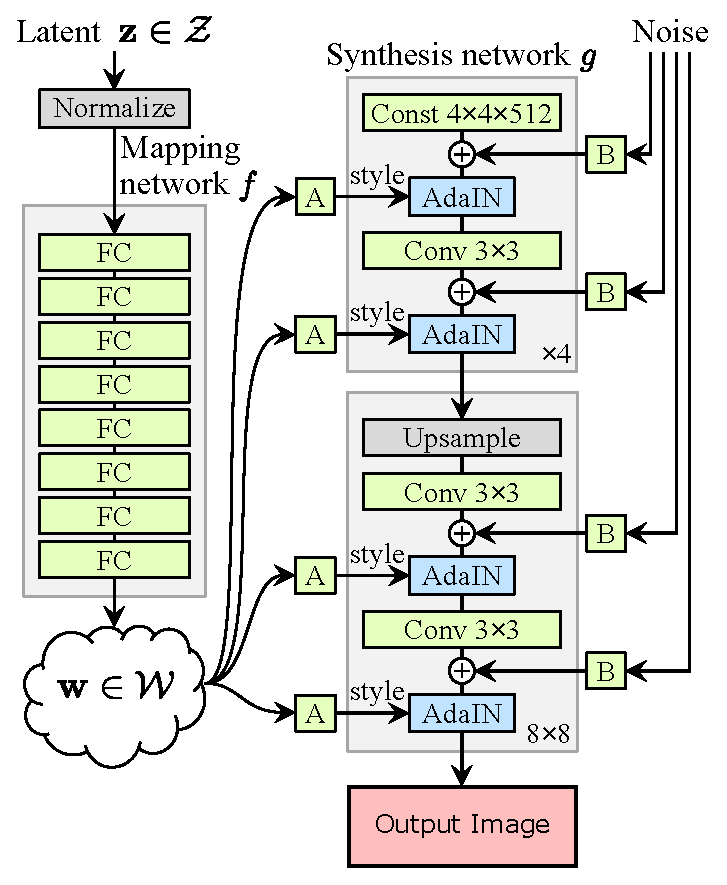
\includegraphics[width=0.75\linewidth]{figures/StyleGAN.eps}
  \caption{StyleGAN architecture for generation of a face image. Adapted from \cite{karras2019style}.}
  \label{fig:styleGAN}
\end{figure}

In case you cannot find the paper on arXiv, you can try to export the figure from the pdf or rebuild it. Taking a screenshot of the figure at the highest possible resolution works for presentations, but will lack quality in the printed version. 

\section{Tables}

Contents of a table can often be grouped. As illustrated by \autoref{tab:results}, vertical lines are not really necessary for that. Moreover, vertical lines often let the table seem overloaded. This is also described by the layout principle ''\textit{Less is more}''. Take a look at this \href{https://inf.ethz.ch/personal/markusp/teaching/guides/guide-tables.pdf}{Small Guide to Making Nice Tables}.
The best results for each metric should be made \textbf{bold}. Besides, note that the caption (in comparison to the figures) is above the table. 

If you work with Excel, \href{https://ctan.org/pkg/excel2latex}{this package} might be helpful for automatically generating \LaTeX -code. 

\begin{table}[H]
\caption{Results of metric 1, 2 and 3 in percent of our proposed methods in comparison with 3 baseline methods on benchmarks 1 and 2.}
\label{tab:results}  
\centering
\small
    \begin{tabular}{lLLLLRL}
    \toprule
          &      \multicolumn{2}{c}{Benchmark 1}     &      \multicolumn{4}{c}{Benchmark 2}     \\
          
\cmidrule(lr){2-3} \cmidrule(lr){4-7} 
          
    Method & \text{Metric 1} & \text{Metric 2} & \text{Metric 1} & \text{Metric 2} &  \multicolumn{2}{c}{Metric 3}  \\
    \midrule
    Baseline 1 \cite{baseline1} & 37.0    & \phantom{0}0.0     & 28.3  & \phantom{0}0.0     & \multicolumn{2}{C}{73.6}    \\
    Baseline 2 \cite{baseline2} & 84.1  & 36.9  & 81.3  & 29.9  & \multicolumn{2}{C}{93.1}  \\
    Baseline 3 & 85.2  & 60.1  & 83.6  & \textbf{57.2} & \multicolumn{2}{C}{-}   \\
        \midrule
    Ours 1 & 87.2  & 57.3  & 85.3  & 39.9  & 67.1 & \textbf{94.5} \\
    Ours 2 & \textbf{87.4} & \textbf{61.2} & \textbf{85.8} & 42.6  & 63.1 & 91.7  \\
    \bottomrule
    \end{tabular}%
\end{table}%

\section{Equations}
Number equations consecutively with equation numbers in parentheses. Make sure you follow the guidelines from \autoref{sec:notation}. Also, explain all used variables. When using vectors/matrices state the dimensions.

The scalar output $y$ of a single neuron with the activation function $\phi\left(\cdot\right)$ is defined as follows:
\begin{equation}
  y = \phi\left(\boldsymbol{w}^{\text{T}}\boldsymbol{x} + b\right)
  \label{eq:neuron}
\end{equation}
with the scalar $b$ denoting the bias, and $\boldsymbol{w}, \boldsymbol{x} \in \mathbb{R}^{512 \times 1}$ being the weight and the input of vectors of the neuron.

Note that there is no indentation as the sentences before and after the equation are connected. If you do not need to explain further variables, leave an extra line to start a new paragraph (with indentation).

\section{Captions}
Every figure needs to have a brief caption describing the figure/table. Do not write too much and keep it short. You should highlight the details and interpret them in the written text only. In contrast to the caption of a figure, the caption of the table is above the table. 


\section{Referencing}
All figures/tables need to be referenced in the written text. For convenience, use \verb'\autoref{fig:styleGAN}' to reference figures. This automatically adds the type of reference in front of the number:
\begin{itemize}
  \item \autoref{fig:styleGAN}
  \item \autoref{tab:results}
  \item \autoref{eq:neuron}
  \item \autoref{sec:notation}
  \item \autoref{ch:template_info}
\end{itemize}


\section{Clean Bibliography}

Every claim you make in the thesis must be verified by either your results or a citation. For details on how and what to cite please take look at \href{https://www.ub.tum.de/en/citation-guide}{TUM Citation Guide}. \textbf{If you fail to provide the source of a figure your thesis can be graded as fail 5,0 due to plagiarism.} Therefore, I recommend to always write down your source when you take a figure from another paper such that you will not forget citing it. You are on the safe side if you make all your figures by yourself. This also allows you to have an overall more consistent notation throughout the thesis. In the related work and background chapter, it is also fine to take figures from other papers (and improve them), but the source needs to be named! Examples are \autoref{fig:styleGAN} and \autoref{fig:faces}.

Go to \href{https://scholar.google.com/}{Google Scholar} and search for the paper you want to cite. You can copy the bibtex entry from there directly to your bibliography file so that all the references have the same look. 

Do not change the bibliography style. The first letter of the last name of the authors together with the last two digits of the year of publication should appear in the reference. Like this: \cite{baseline1} (= [EAO19])

Make sure the bibliography is consistent!
Never forget to mention author(s), title, year and where the article was published. Also, make sure every conference is formatted the same way and the title is written (capitalized) as in the paper (double \{\{Title you Want to Cite\}\} will do the job).

\section{\LaTeX\ Literature}
\label{sec:literature}
You will find many \LaTeX-tutorials searching the internet. Besides,   \cite{Ko03} is a quite comprehensive book, of which the library has adequate stock.

% Introduction
\chapter{Introduction}
\label{ch:introduction}

\section{Motivation}
With the recent release of StabilityAI's Open Model Stable Diffusion 3 \cite{esser2024scalingrectifiedflowtransformers}, latent diffusion models have pushed the boundaries of creating more realistic images even further. However, training these general-purpose models is extremely expensive, and they may reach a plateau where further enhancements require exponentially more data, as noted by \cite{udandarao2024zeroshotexponentialdatapretraining}. Therefore, the focus should shift towards optimizing the use of existing models for specialized tasks and exploring new scientific fields where these models can be as effective as they are in other domains.

One example is the field of computer vision, which by itself has revolutionized numerous other fields, from autonomous driving and healthcare to surveillance and entertainment. Developing robust and accurate computer vision models often depends on the availability of high-quality, diverse datasets. Real-world data collection can be extremely expensive, time-consuming, and sometimes infeasible due to privacy concerns or safety issues. Consequently, synthetic data has become an important resource for bridging this gap.

Synthetic data offers high flexibility, enabling researchers to generate vast quantities of labeled images under controlled conditions. This controlled environment captures necessary variations, such as different lighting conditions, weather scenarios, and camera perspectives, which are often challenging to achieve with real-world data collection. Despite these advantages, synthetic data can lack the realism required to effectively train and evaluate high-performance models \cite{zhou2017unsupervisedlearningdepthegomotion}.

Diffusion models could solve this problem, offering the capability to enhance synthetic image data, making it a more realistic representation of reality while retaining the advantage of complete control over the test environment. The resulting datasets enable training on rare events, improving the robustness of detection and tracking systems and allowing training in scenarios where real data is unavailable.

\section{Problem Description}
\label{sec:prob_description}
Synthetic data is essential for many computer vision tasks where real data is unavailable or limited, such as object detection and tracking. This thesis aims to utilize pre-trained neural networks and extensions based on Stable Diffusion \cite{rombach2022highresolution} to create a pipeline that transforms existing (synthetic) data from Synthehicle \cite{Herzog_2023_WACV} and the MUAD Dataset \cite{Franchi2022MUAD} into high-variance realistic data. Synthehicle and other synthetic datasets provide semantic, instance, and depth ground truth, which can be used as image conditions in diffusion networks. In this work, the recently proposed ALDM \cite{li2024aldm} network with other post-processing operations will be used to produce images that are: 
\begin{itemize}
    \item realistic, 
    \item high-variance (in terms of weather, lighting, and overall scene conditions) and 
    \item consistent with the ground truth labels. 
\end{itemize}

\section{Contribution} 
The main contributions of this thesis are:
\begin{itemize}
    \item Implementation of a diffusion pipeline based on ALDM \cite{li2024aldm} that transforms existing
synthetic and real images as described above, and other enhancement methods, primarily using image-to-image technology guided by different ControlNets.
    \item Conducting a comprehensive analysis of the influence on performance when the generated data
is used as training data for video analysis tasks focusing on object detection.
    \item Conduction tests around spatial-temporal image consistency, especially focusing on object tracking.
    \item Discussion of potentials and limitations of diffusion-based synthetic data generation and how
certain emerging problems could be resolved.
\end{itemize}

\section{Structure}

\subsection{Background}
This chapter covers the foundational concepts and technologies relevant to the thesis. It includes detailed explanations of various neural network architectures, such as Artificial Neural Networks (ANNs), Convolutional Neural Networks (CNNs), Recurrent Neural Networks (RNNs), Transformer Models, Generative Adversarial Networks (GANs), and Latent Diffusion Models. It also discusses encoder-decoder structures and the ControlNet.

\subsection{Related Work}

This chapter reviews existing literature and previous work related to the thesis topic. It discusses various projects and models, such as Synthehicle \cite{Herzog_2023_WACV}, Adversarial Supervision Makes Layout-to-Image Diffusion Models Thrive (ALDM) \cite{li2024aldm}, the paper "Applications of generative AI for sim-to-real data synthesis in driving" \cite{zhao2024exploring}, the CARLA simulator \cite{dosovitskiy2017carlaopenurbandriving}, and Yolo \cite{redmon2016lookonceunifiedrealtime} with its predecessor YoloX \cite{yolox2021}.

\subsection{Own Work}
This chapter details the research and contributions of this paper. It includes the project structure and functionality of the developed Stable Diffusion Pipeline. It also provides an in-depth look at the different modules created and describes the testing setups for object detection on the resulting images, as well as the consistency of resulting videos and object tracking.

\subsection{Evaluation}
This chapter presents the evaluation of the research work. It includes an assessment of ALDM \cite{li2024aldm} and image-to-image transformations regarding object detection and object tracking. The chapter also evaluates spatial-temporal image consistency and discusses diffusion-based synthetic data findings, potentials, and limitations.

\subsection{Conclusion and Outlook}
This final chapter summarizes the key findings and contributions of the thesis. It also suggests potential areas for future research, building on the results and insights gained from the current work.

% Background
\chapter{Background}
\label{ch:background}

\section{Artificial Neural  Networks}
\label{sec:ann}
An artificial neural network (ANN)  \cite{rashid2016make} \cite{youtube3blue1brown}  \cite{zhang2023dive} describes the architecture of neurons and their connection,  which is orientated towards biological neurons to simulate a learning process. 

ANNs consist of multiple layers, each of them containing a large number of neurons. The input layer consists of a node for each part of its input (e.g., a greyscale picture with the size of 400 x 400 pixels could contain 160,000 input nodes, one node for each pixel with an input between 0 and 255). The output layer is the last layer where the number of neurons maps directly to the desired output (e.g., if you want to decide if the animal in the picture is a dog or a cat, you could use one final neuron - if it activated, the ANN detected a cat, otherwise a dog). All layers in between are called hidden layers because they are not influenced by the outside. Each neuron has an activation function, determining if a neuron is activated by its input. Every neuron in layer $k$ can get its input from other neurons' output from the layer $k-1 = j$. An edge between two neurons has a weight $w^{jk}$ assigned, influencing the sum of all the inputs from this edge. In mathematical terms, an artificial neuron is described by a function, also called an activation function. Over a layer's potentials and weights of the edges, a weighted sum is formed and projected via the activation function into a smaller space. Two often used functions are the Sigmoid function which projects all values into the interval $(0, 1)$
\begin{equation}
{\phi (\mathbf{v} )=(1+\exp(- \mathbf {v}))^{-1}}
\end{equation}  
and the ReLU function, projecting to $[0, \infty)$:
\begin{equation}
\phi (\mathbf{v}) = \max(0, \mathbf{v})
\end{equation}.
Also, a bias ($\beta$) could be added to shift neurons activation potential. 

To calculate the output of a neural network, a neuron's activation potential could be written down as a vector, multiplied by a matrix containing every edge that leads to the nodes in layer $k$. One row in the matrix corresponds to the edges between a neuron in layer $j$ and a particular neuron in layer $k$. After that, a bias is added, and everything is wrapped into an activation function again, leading to the next node's potential \cite{youtube3blue1brown} \cite{zhang2023dive}:
\begin{equation}
\label{eq:ann_forward_propergation}
\boldsymbol{H}^{k} = \phi \left(
\begin{bmatrix}
w^{jk}_{0,0} & w^{jk}_{0,1} & \cdots & w^{jk}_{0,m}\\
w^{jk}_{1,0} & w^{jk}_{1,1} & \cdots & w^{jk}_{1,m}\\
\vdots  & \vdots  & \ddots & \vdots \\
w^{jk}_{n,0} & w^{jk}_{n,1} & \cdots & w^{jk}_{n,m} \\
\end{bmatrix}
\cdot
\begin{bmatrix}
a_{0}^{j}\\
a_{1}^{j}\\
\vdots \\
a_{2}^{j}\\
\end{bmatrix}
+
\begin{bmatrix}
\beta_{0}^{j}\\
\beta_{1}^{j}\\
\vdots \\
\beta_{2}^{j}\\
\end{bmatrix}
\right) 
\xrightarrow{\text{}}
\boldsymbol{H}^{k} = \phi{(\boldsymbol{W}^{jk}\boldsymbol{A}^j + \boldsymbol{\beta}^j)}
\end{equation}
To make ANNs effective in predicting outputs, they have to be trained. "Backpropagation" describes the process of training the model to minimize the total cost by each output (or batch). For every result, the cost (also called "loss" or "error") in the output layer $c_n$ is calculated by subtracting the actual output $a_n$ from node $n$ by the expected output $e_n$. Squaring the result for an individual node and taking the sum over all nodes results in the cost of one run. For all nodes, the cost is:
\begin{equation}
\vect{c} = 
\begin{bmatrix}
(e_{1} - a_{1})^{2}\\
(e_{2} - a_{2})^{2}\\
\vdots \\
(e_{n} - a_{n})^{2}\\
\end{bmatrix}
\end{equation}
The average cost of multiple runs describes the performance of a neural network. 
Finding the global minimum of the cost function could be an option to minimize the cost. The problem with this approach is that the calculation cost is too high, making even calculations for small networks inefficient. Therefore, "gradient descent" is used, which approaches a local minimum iteratively. For backpropagation, the sensitivity of the cost function for a neuron with respect to every connected weight (and biases) is interesting because it represents the slope of the error function. The question is, how much do the weights of the edges have to be changed to correct the output. Mathematically speaking \cite{zhang2023dive}, this is denoted by:

\begin{equation}
\frac{\partial{\vect{c}}}{\partial{\boldsymbol{W}^{jk}}}
\end{equation}
Looking at the network error function with the idea in mind that only the errors from the nodes that the neuron is connected to is interesting, the formula can be reformulated to: 

\begin{equation}
\frac{\partial{\vect{c}}}{\partial{\boldsymbol{W}^{jk}}} = \frac{\partial}{\partial{\boldsymbol{W}^{jk}}} +  \vect{c}^k
\end{equation}
As mentioned above the indices $j$ and $k$ reference the different layers, where $\boldsymbol{W}^{jk}$ is a matrix containing the weights connecting layer $j$ and $k$. In the calculation, it is also assumed that $k$ represents the final layer. Looking at $\vect{c}^k$, it is known that $\vect{e}^k$, the expected output, is not dependent on the function. With the chain rule and building the resulting derivatives, the following term emerges:

\begin{equation}
\frac{\partial{\vect{c}}}{\partial{\boldsymbol{W}^{jk}}} = \frac{\partial{\vect{c}}}{\partial{\vect{a}^k}}
\cdot \frac{\partial{\vect{a}^k}}{\partial{\boldsymbol{W}^{jk}}} = -2\vect{c}^k \cdot \frac{\partial{\vect{a}^k}}{\partial{\boldsymbol{W}^{jk}}}
\end{equation}

The second part of the equation heavily depends on the activation function because $a^k$ is the activation of the node in layer $k$, in this case, in the final layer, and is calculated by $\phi(\sum_j \boldsymbol{W}^{jk} \cdot \vect{a}^j)$. Calculating the derivative of the last term with the chain rule results in:

\begin{equation}
\frac{\partial{\vect{c}}}{\partial{\boldsymbol{W}^{jk}}}
= -2\vect{c}^{k} \cdot \phi'\left(\sum_j \boldsymbol{W}^{jk} \cdot \vect{a}^j\right) \cdot \frac{\partial}{\partial{\boldsymbol{W}^{jk}}} \vect{a}^k 
= -2\vect{c}^{k} \cdot \phi'\left(\sum_j \boldsymbol{W}^{jk} \cdot \vect{a}^j\right) \cdot \vect{a}^j
\end{equation}
This is the formula to calculate the change for the weights connecting the output. With the small modification of removing the factor $2$ (when adding the direction to the weight later, it is scaled via a new factor also called "learning rate") and looking at $\vect{c}^k$ as the error of layer $k$ (which is calculated by taking multiplying the transformed nodes from any layer $k$ with the weights from $jk$), with $j$ and $k$ being an arbitrary layer, this results in the final function for updating the weights:
\begin{equation}
\frac{\partial{\vect{c}}}{\partial{\boldsymbol{W}^{jk}}}
= -\vect{c}^{k} \cdot \phi'\left(\sum_j \boldsymbol{W}^{jk} \cdot \vect{a}^j\right) \cdot \vect{a}^{j}
\end{equation}
For updating weights, the calculation is
\begin{equation}
\boldsymbol{W}^{jk} = \boldsymbol{W}^{jk} - \alpha \cdot \frac{\partial{\vect{c}}}{\partial{\boldsymbol{W}^{jk}}} 
\end{equation}
with $\alpha$ being the above-mentioned learning rate. Implementing such a neural network heavily relies on matrix multiplications which can be calculated very efficiently, especially with the help of modern graphic cards. Because of this, ANNs are in use to this day, often in combination with other network types that are presented below \cite{yolox2021} \cite{vaswani2023attentionneed}.

\section{Convolutional Neural Networks}
Conventional Neural networks (CNNs) \cite{oshea2015introductionconvolutionalneuralnetworks} are another type of network and are often combined with ANNs. They are used to extract features from an image by applying different "filters" to it. 

A CNN consists of multiple layers as well. Like an ANN, a CNN typically includes an input layer with a size corresponding to the number of pixels in the input image and maps to a much smaller number of nodes. In a CNN, the activation of a neuron depends on a learnable kernel. A kernel is a matrix that convolves over the input vector, aiming to extract important features while diminishing unimportant ones. Convolution involves selecting a pooled vector $\boldsymbol{p}$, usually represented as a quadratic matrix $\boldsymbol{P}$ with a center value $c$, and a quadratic kernel $\boldsymbol{K}$. The pooled vector and kernel are multiplied together via the dot product, with the resulting value replacing $c$ in the input vector. Through backpropagation, the kernel is trained to improve performance. \cite{oshea2015introductionconvolutionalneuralnetworks}

Due to performance reasons, a CNN is often used to map a large input to a smaller dimension by adjusting the depth, the stride, and zero padding. Depth describes the number of convolution layers (a reduction leads to fewer neurons for the cost of recognition performance), the stride is the distance around different center points, and zero-padding is the \textit{"simple process of padding the border of the input"} \cite{oshea2015introductionconvolutionalneuralnetworks}.

Another way to reduce the output size is by using a pooling layer. In pooling layers, a kernel (typically 2 x 2) is used with a larger stride than $\frac{width_{\text{kernel}}}{2}$ to further minimize the output array. Only the largest number within the pooled vector is carried to the next layer for max pooling. Pooling layers can also be used for other optimizations, such as L1/L2 normalization \cite{Wu_2019} \cite{gholamalinezhad2020poolingmethodsdeepneural} and average pooling \cite{gholamalinezhad2020poolingmethodsdeepneural} \cite{oshea2015introductionconvolutionalneuralnetworks}.

\section{Autoencoder}
\label{sec:autoencoder}
The Autoencoder architecture describes a possible solution for compressing high dimensional data to lower dimensions (encoder) and rebuilding it with information, the encoder removed (decoder). The idea was first proposed in the paper "Fully Convolutional Networks for Semantic Segmentation" \cite{long2015fullyconvolutionalnetworkssemantic} as an efficient upsampling method after downsizing an image by a CNN.

As mentioned above, autoencoders reduce their input to a much smaller space, known as the "latent space". It later upscales the vector in the smaller space again to a possible new domain, such as segmentation maps for image classification. The downscaling/encoding is performed by a CNN, consisting of multiple kernel and pooling layers. In modern autoencoders, these memorized pooled indices are filtered by a \textit{"trainable filter bank"}\cite{badrinarayanan2015segnetdeepconvolutionalencoderdecoder} and later injected into the decoding process to get lost information by the encoding process back into the image. The decoder is also a CNN with small modifications, often called a "deconvolution network". Instead of convolution, deconvolution takes a smaller input and expands it into a larger output with the help of a trainable kernel. The pooling layers are reversed with the help of the filter bank.

An implementation of this approach, which is used to this day is the "UNET" \cite{ronneberger2015unetconvolutionalnetworksbiomedical}. For the encoder part the network uses \textit{"two 3x3 convolutions (unpadded convolutions), each followed by
a rectified linear unit (ReLU) and a 2x2 max pooling operation with stride 2"} \cite{ronneberger2015unetconvolutionalnetworksbiomedical} doubling the number of feature channels (each kernel produces an output for each input, which results in $\text{fchannels}_{\text{output}} = 2 \cdot \text{fchannels}_{\text{input}}$). The decoder part reverses this process, but instead of injecting the data via a "filter bank", it concatenates the corresponding feature map to each layer. It bisects it afterward via deconvolution. That results in the decoder side having one additional convolution, reducing the "feature channels" without any concatenation to its final result.

\begin{figure}[H]
  \centering
  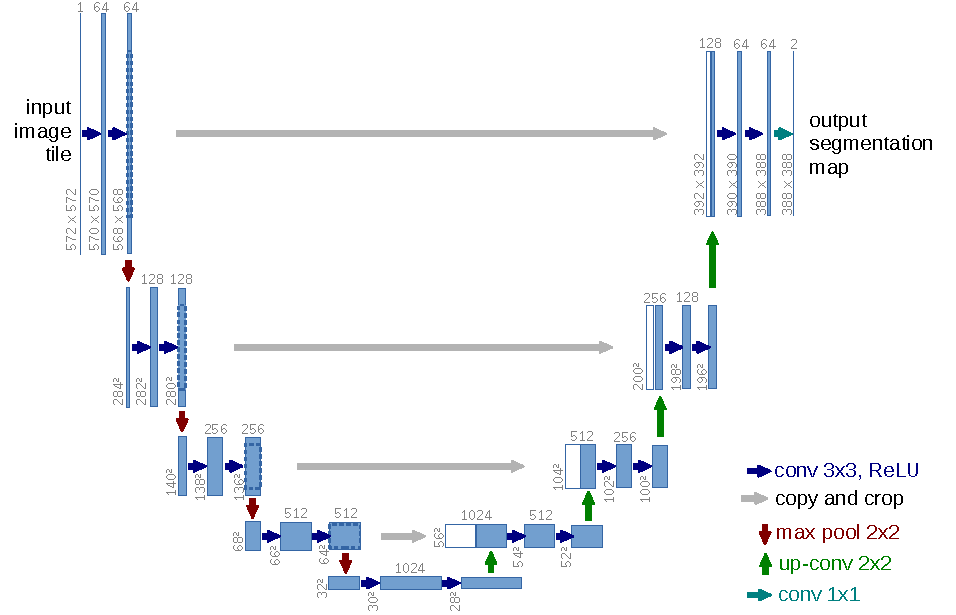
\includegraphics[width=\textwidth]{figures/background/u-net-illustration-correct-scale2.pdf}
  \caption{Structure of the UNET architecture. \cite{ronneberger2015unetconvolutionalnetworksbiomedical}}
  \label{fig:unet}
  \clearpage
\end{figure}

\section{GAN}
\label{sec:gan}
Generative Adversarial Net (GAN) \cite{goodfellow2014generativeadversarialnetworks} is an architecture for generating and validating images through a second instance. A generative model, $G$, and a discriminative model, $D$ are trained together with $G$ generating data to fool $D$. $D$ distinguishes between "real" (Data from the training set) and generated, often called "fake" data. Both models are trained using backpropagation, avoiding complex inference methods. Various experiments demonstrate \cite{zhao2024exploring} \cite{karras2018progressivegrowinggansimproved} that this adversarial process drives $G$ to produce realistic data. 

This raises the question: what are the advantages of playing such a game, and why not simply predict every pixel individually to produce a completed picture? This approach also exists, and these frameworks are called "Autoregressors" \cite{oord2016pixelrecurrentneuralnetworks}. They can be trained by removing information from an image and letting the model predict the missing information. The problem with this approach lies in the complexity of image generation. While generating embedding after embedding up to a few hundred is fine, generating a few million pixels is slow. The problem with developing a more significant number of pixels simultaneously is that Neuronal networks average their output, resulting in a blurry result. 

GANs, therefore, play their adversarial game with the discriminator, allowing generation in one passthrough starting with a random vector.

Looking at the adverse game inside a GAN from a mathematical perspective, to calculate the loss for such a framework, the following value function is important: \cite{goodfellow2014generativeadversarialnetworks}:

\begin{equation}
\label{eq:minimaxgame-definition}
\mathcal{L} = \min_G \max_D V(D, G) = \mathbb{E}_{x \sim p_{\text{data}}(x)}[\log D(x)] + \mathbb{E}_{z \sim p_{z}(z)}[\log (1 - D(G(z)))]
\end{equation}

where $G$ marks a parameterized function and $D$ the discriminator, a function returning a scalar. The first part of the equation

\begin{equation}
\min_G \max_D V_I(D, G) = \mathbb{E}_{x \sim p_{\text{data}}(x)}[\log D(x)]
\end{equation}

maximizes $D$ for a given element from the data, and the second part

\begin{equation}
\min_G \max_D V_{II}(D, G) = \mathbb{E}_{z \sim p_{z}(z)}[\log (1 - D(G(z)))]
\end{equation}

minimizes $D$ for $G$ from $D$'s perspective and maximizes $D$ from $G$'s perspective if the image is a "fake". 


\section{Recurrent Neural Networks}

Recurrent Neural Networks (RNN) \cite{zhang2023dive} enlarge ANNs by allowing each neuron to input its previous output again and thus maintain its state. Therefore, RNNs are well-suited for tasks like natural language processing, time series prediction, and speech recognition.

Looking into this from a mathematical point of view, the goal is to predict a token $x$ at time $t$ with a set of tokens that were injected into the model before $t$. They are denoted as $x_{t - n}$ with $n \in \mathbb{N} \land t - n > 0$. Because it would be computationally too expensive to store a state of the network for each token, all of them are combined into a hidden state $h$. A hidden state is defined as a state inside a neuronal network that can only be calculated recursively on top of the previous result:

\begin{equation}
\mathbb{P}(x_t | x_{t - 1}, ..., x_0) \approx \mathbb{P}(x_t | h_{t-1})
\end{equation}
Extending \autoref{eq:ann_forward_propergation} by the inner state with extra weights for control leads to: 

\begin{equation}
    \boldsymbol{H}_t = \phi{(\boldsymbol{W}_{l}^{j-1}\boldsymbol{A} + \boldsymbol{W}_{s}^{j}\boldsymbol{H}_{t-1} + \boldsymbol{\beta}^{j-1})}
\end{equation}
One of the problems of this approach is that for each iteration the weight $\boldsymbol{W}_{s}^{j}$ is multiplied again to $\boldsymbol{H}$. If this weight is larger than $1$, over time, it leads to large gradients, also called gradient explosion. On the other hand, if it is smaller than $1$, it leads to gradient vanishing \cite{zhang2023dive}. For that reason, RNNs were modified to different forms like long short-term memory \cite{zhang2023dive} \cite{hochreiter1997lstm} and gated recurrent networks \cite{chung2014empirical}, which use memory cells and gates to maintain and regulate information across long sequences.

\section{Transformer Models \& Self Attention}
\label{sec:transformer_models_and_self_attention}
As mentioned above, the biggest problems regarding recurrent neural networks are gradient vanishing and explosion and not memorizing features over a large context size \cite{zhang2023dive}. 
To counter this, attention was created, an approach that allows finding features in early tokens and memorizing them over a long time. It was combined into a transformer, a deep-learning architecture proposed by researchers at Google. This architecture, unlike its predecessors, only uses attention to maintain its state, which increases performance regarding translation tasks and later led to the creation of Large Language Models \cite{brown2020language}, as well as cross-attention and backbone architectures for latent diffusion algorithms
\cite{rombach2022highresolution} \cite{peebles2023scalablediffusionmodelstransformers}. 

A transformer has two different parts: an encoder and a decoder \autoref{sec:autoencoder}. In this architecture, the encoder and decoder have a defined size of stacks, where each stack is again divided into two sub-layers, with the first being a multi-head self-attention mechanism and the second being a simple, position-wise, fully connected feed-forward network \autoref{sec:ann}. The decoder adds a third sub-layer to each stack, which performs multi-head attention over the output of the encoder stack and also masks the output tokens to not influence previous ones.\cite{vaswani2023attentionneed}  

The core of the transformer model is the attention mechanism, which aims to enhance a token with the meanings of the other tokens around it. The idea is to map the tokens from the high dimensional embedding space to a smaller Query/Keyspace and multiply the attention pattern to the embedding. A query $\vect{q}_1$ is calculated by multiplying a matrix $\boldsymbol{W}_Q$, consisting of tunable parameters, with the token vector of an embedding $\boldsymbol{e_i}$. A key is calculated the same way, but instead of multiplying $\boldsymbol{W}_Q$ with the embedding, the key matrix $\boldsymbol{W}_K$, another matrix consisting of tunable parameters is used. After that, a new matrix is calculated by multiplying the dot product of each resulting key-value pair and multiplying it with the corresponding $\vect{v}_k$, resulting from multiplying another tunable matrix $\boldsymbol{W}_V$ by each embedding vector. $\boldsymbol{W}_V$ is normally split into two smaller matrices, as you can see later. \cite{vaswani2023attentionneed} \cite{youtube3blue1brown}

\begin{equation}
    \text{Attention}(\boldsymbol{Q}, \boldsymbol{K}, \boldsymbol{V}) = \text{softmax}\left(\frac{\boldsymbol{Q}\boldsymbol{K}^T}{\sqrt{d^k}}\right)\boldsymbol{V}
\end{equation}

$\boldsymbol{Q}$, $\boldsymbol{K}$ and $\boldsymbol{V}$ are vectors containing $[\boldsymbol{q}_1, \boldsymbol{q}_n]$, $[\boldsymbol{k}_1, \boldsymbol{k}_n]$ and $[\boldsymbol{v}_1, \boldsymbol{v}_n]$, while $\frac{1}{\sqrt{d^k}}$ counters the effect of the dot products growing large in magnitude and therefore \textit{"pushing the softmax function into regions where it has extremely small gradients"}. \cite{vaswani2023attentionneed}. As mentioned above, masking is also applied so that succeeding tokens do not influence previous tokens, as the goal of a transformer is to predict these. To preserve the normalized columns calculated by the softmax function, all entries in $\boldsymbol{Q}\boldsymbol{K}^T$ representing the influence of a succeeding token are set to infinity. \cite{vaswani2023attentionneed}

For each token, the influences resulting from $\text{Attention}(\boldsymbol{Q}, \boldsymbol{K}, \boldsymbol{V})$ are added up, resulting in $\Delta e_i$. This marks the change, which is added to $e_i$.

To make this idea computationally more efficient, these attention heads and their corresponding changes are calculated multiple times in parallel, each attention head with its own $\boldsymbol{Q}, \boldsymbol{K}, \boldsymbol{V}$:

\begin{multline}
    \text{MultiHead}(\boldsymbol{Q}, \boldsymbol{K}, \boldsymbol{V}) = \text{Concat}(head_1, ..., head_h)\boldsymbol{W}^{O}  \\ 
    \text{where } head_i = \text{Attention}(\boldsymbol{QW}^{Q}_{i} , \boldsymbol{KW}^{K}_{i}, \boldsymbol{VW}^{V}_{i} )
\end{multline}

where $\boldsymbol{W}^{O} \in \mathbb{R}^{hd_v \times d_\text{model}}$, $\boldsymbol{W}^{V} \in \mathbb{R}^{d_\text{model} \times d_v}$ and $h$ the number of attention layers. The previous matrix $\boldsymbol{W}^K$, which also exists $h$ times, is split up into $\boldsymbol{W}^{O}$ (also called Output Matrix) and $\boldsymbol{W}^{V}$, where only $\boldsymbol{W}^{V}$ is part of the attention mechanism. With this mechanism, calculating the weighted sums on the smaller matrices from $W^{O}$ and multiplying $W^{V}$ is much less computationally difficult.\cite{vaswani2023attentionneed} \cite{youtube3blue1brown} \cite{elhage2021mathematical}.

Every layer also consists of a Fast Forward Neuronal Network (FNN, a term equivalent to ANN \autoref{sec:ann}). The dimensions of this network's input and output layer are $d_\text{model}$. It also has a larger hidden layer, which in the implementation of this paper \cite{vaswani2023attentionneed} is scaled by factor $4$.

While transformer models' most famous usage today is in "Generative Pretrained Transformers" like GPT-3 \cite{brown2020language}, most diffusion algorithms, see \autoref{sec:latent_diffusion_models} use attention mechanisms to extract meaning out of text embeddings for image generations.

Also, despite one of the biggest problems Transformers have, being their context size growing by the factor ${\text{input}^2}$ ($\text{embeddings} \cdot \text{query}, \text{embeddings} \cdot \text{key}, \text{embeddings} \cdot \text{output-matrix}$), there are implementations of modern diffusion models using transformers to replace the UNET \cite{ronneberger2015unetconvolutionalnetworksbiomedical} \cite{peebles2023scalablediffusionmodelstransformers}.

\section{Latent Diffusion Models \& Text to Image}
\label{sec:latent_diffusion_models}

Instead of using GANs to generate high-quality images, (latent) diffusion models could also be used. The idea of diffusion models is to counter the blurring when generating too many images simultaneously by decoupling pixels so that they are independent of each other. This is done by adding random noise. Mathematically speaking, having an image $x_0$, in the encoding process, noise $\epsilon \sim  \mathcal{N}(0, 1)$ is applied $T$ times onto the image resulting in $x_T$. In every iteration, more noise gets added. The following interpolation can calculate each intermediate step $x_t$:

\begin{equation}
x_t = \left(\frac{T - t}{T}\right) \cdot \epsilon  + \left(1 - \frac{T - t}{T}\right) x_0
\end{equation}

The decoder is a function $\mathcal{E}_\theta$ with trained parameters to revert the noise added by the encoder step by step. This is done via the UNET \cite{peebles2023scalablediffusionmodelstransformers}, which is described above. To speed up this process during the training phase, evaluation of the result from denoising $x_t$ is not done against $x_t - 1$ but against $x_0$, or to be more exact, it predicts the noise $\epsilon_t$ until $\epsilon_0$. This is really efficient because that way, the model only learns how to denoise to a clean image and not all steps in between (this does not mean that denoising is done in one step later - it is only trained to do it in one step). Looking at the loss function, it is calculated as the "Mean Squared Error" between the actual noise applied and the current image $x_t$, which is, as mentioned above, put together out of noise $\epsilon_t$ and $x_0$.

The problems resulting from this approach are the long generation time (one denoising step equals one iteration through the network) and the large amount of training data needed to make the algorithm learn efficiently. To counter both of these problems, Robin Rombach proposed in his infamous paper "High-Resolution Image Synthesis with Latent Diffusion Models" \cite{rombach2022highresolution} to shift calculation from the pixel space to the latent space of the UNET, which is looking back at \autoref{fig:unet} at the bottom of the U-Shape.

To train the autoencoder, equivalent to the GAN approach (see \autoref{sec:gan}), a discriminator is used to distinguish between "fake" images produced by the autoencoder and the real images from the dataset - the resulting loss function from this approach now combines the diffusion loss function, the discriminator loss function and a third loss function, similar to the loss calculation of variational autoencoder (VAE) \cite{kingma2022autoencodingvariationalbayes}:

\begin{equation}
\mathcal{L}_{\text{Autoencoder}} =  \min_{\mathcal{E}, \mathcal{D}} \max_\psi \left( \mathcal{L}_{\text{rec}}(x, \mathcal{D}(\mathcal{E}(x))) - \mathcal{L}_{\text{adv}}(\mathcal{D}(\mathcal{E}(x))) + \log \mathcal{D}_\psi(x) + \mathcal{L}_{\text{reg}}(x; \mathcal{E}, \mathcal{D}) \right)
\label{eq:firststageloss}
\end{equation}

The diffusion loss is calculated in $\mathcal{L}_{\text{rec}}(x, \mathcal{D}(\mathcal{E}(x)))$, while $\mathcal{L}_{\text{reg}}(x; \mathcal{E}, \mathcal{D})$ is the regularisation of the latent image by taking the encoder output $\mathcal{E}(x) = L$, with $L$ being the image in the latent space and calculate the loss with respect to $\mathcal{N}(0, 1)$. The last two parts of this loss function 

\begin{equation}
\min_{\mathcal{E}, \mathcal{D}} \max_\psi \left(- \mathcal{L}_{\text{adv}}(\mathcal{D}(\mathcal{E}(x))) + \log \mathcal{D}_\psi(x)\right) 
\approx 
\min_{\mathcal{E}, \mathcal{D}} \max_\psi \left(\left[(\mathcal{D}_\psi(\mathcal{D}(\mathcal{E}(x)))) \right] + \log \mathcal{D}_\psi(x)\right)
\end{equation}
are part of the adverse game \autoref{sec:gan} and calculate the loss for minimizing the discriminator's output by adjusting the $\mathcal{D}_\psi$ (detecting that $(\mathcal{D}(\mathcal{E}(x)))$ is a "fake" image) while trying to maximize the discriminator's output by adjusting $(\mathcal{D}(\mathcal{E}(x)))$ (making $(\mathcal{D}(\mathcal{E}(x)))$ looks real). The last part, $\log \mathcal{D}_\psi(x)$, aims to maximize the discriminator's output for real images. Therefore, it is identical to the above described GAN loss function \autoref{eq:minimaxgame-definition}

Combining these two goals of the Latent Diffusion Model denoises the image to its state before and also prevents it from being detected by the discriminator, creating a well-defined latent space and allowing consistent image generation. Instead of running the denoising function $\mathcal{E}_\theta$ on the pixel-space representation $x_T$, it is more feasible to train and run it on the latent-space representation $z_T$ until $z_0$. The loss function is equivalent to the one on the pixel space. The resulting latent representation $z_0$ is afterward put into the decoder to obtain the final image.

The last important part of most of these models is the conditioning. Conditioning is done by concatenating the tokens with the images or by cross-attention. For cross-attention, the input is tokenized/split up (here defined as $\mathcal{T}_\theta$) equivalent to self-attention described in \autoref{sec:transformer_models_and_self_attention}. But instead of mapping tokens to itself, the latent image $z$ is mapped via the Query ${\boldsymbol{W}^{Q_z}}$ to the Keys $\boldsymbol{W}^{K_{\mathcal{T}_\theta}}$ and the Output $\boldsymbol{W}^{V_{\mathcal{T}_\theta}}$. To enhance the influence, classifier-free guidance \cite{ho2022classifierfreediffusionguidance}\cite{dieleman2022guidance} was introduced, where the image is generated two times, one time with and once without the condition, and only the difference is added:
\begin{equation}
z_i = z_{i + 1} + (\mathcal{E}_\theta(z_{i + 1} \oplus \mathcal{T}_\theta) - \mathcal{E}_\theta({z_{i + 1}}))
\end{equation}

Ultimately, the images can upscaled by latent diffusion models via conditioning \cite{rombach2022highresolution}. That allows the diffusion algorithm to generate the image on smaller inputs, resulting in higher calculation speed.

\section{ControlNet}
\label{ch:controlnet}

The ControlNet architecture \cite{zhang2023addingconditionalcontroltexttoimage} aims to enable latent diffusion models with additional conditioning inputs, avoiding the need to retrain parts of the original model, which would add significant computational costs. To achieve this, ControlNet duplicates the encoding layers of the diffusion network, treating each of them as a "trainable copy". The parameters of the original diffusion network are fixed, preventing any modifications, as symbolized by the lock in \autoref{fig:controlnet}.

\begin{figure}[H]
  \centering
  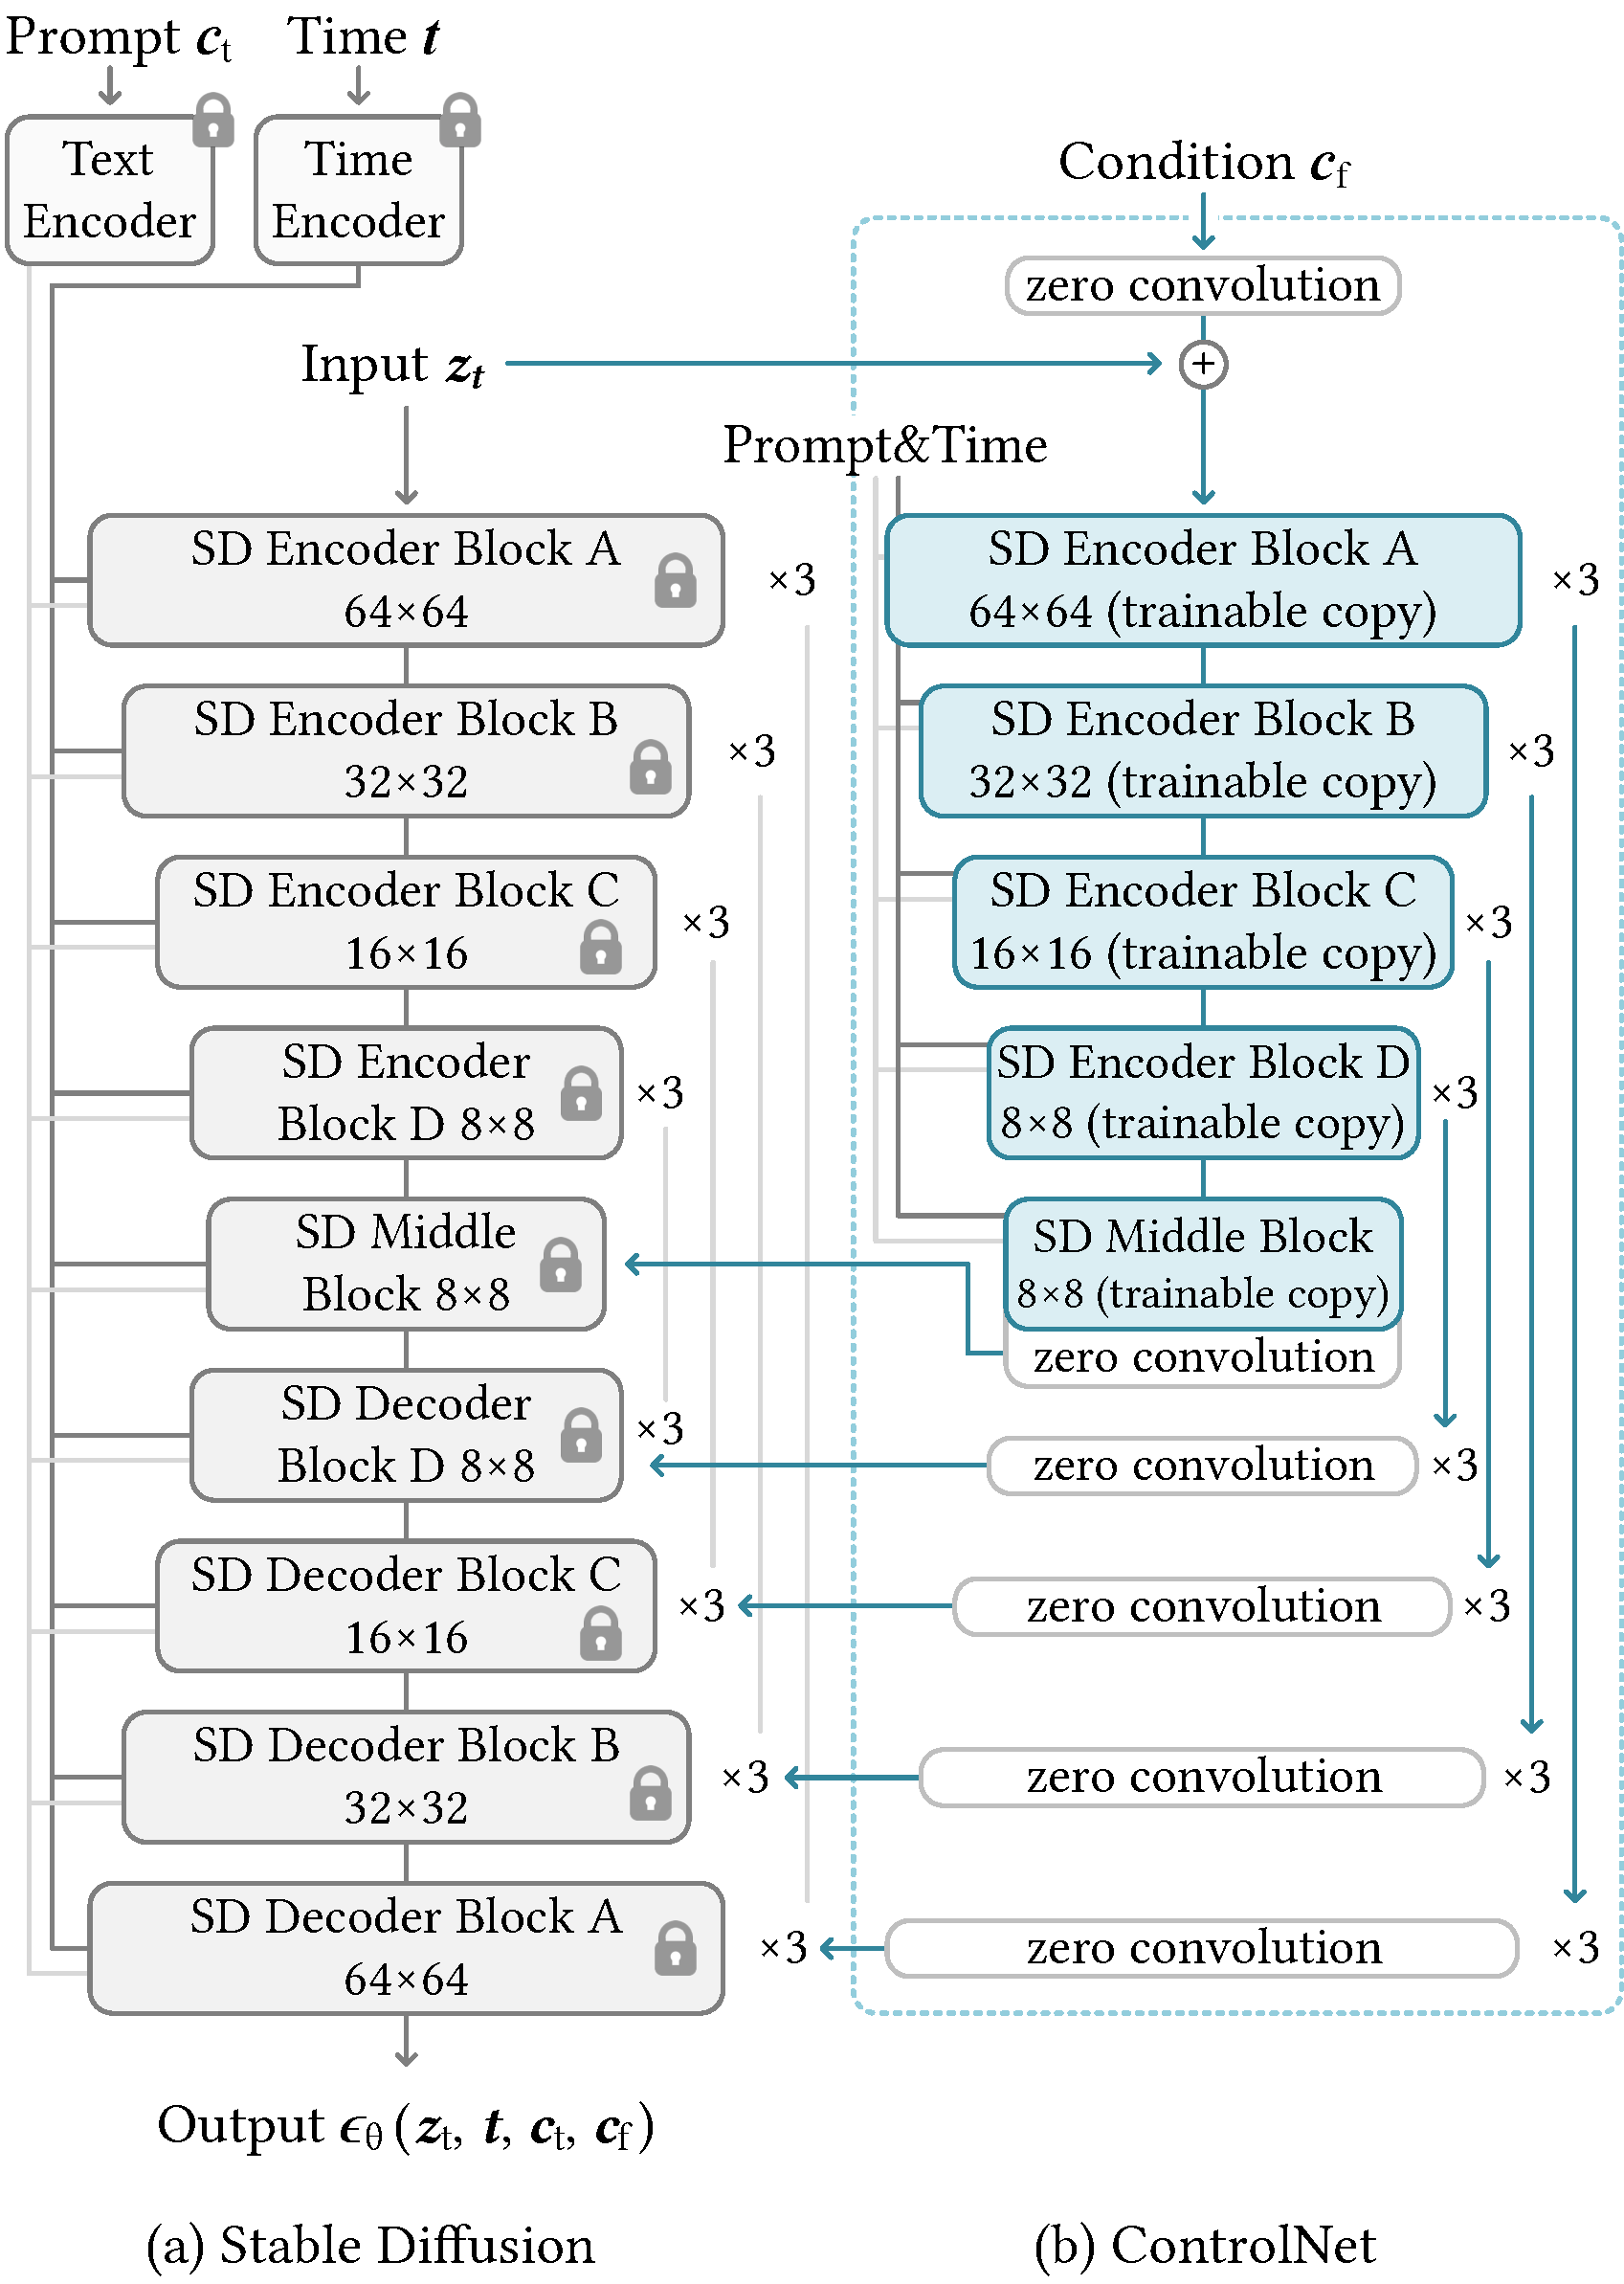
\includegraphics[width=0.5\textwidth]{figures/background/controlnet.pdf}
  \caption{Structure of the ControlNet (right) and the Diffusion Network (left). \cite{zhang2023addingconditionalcontroltexttoimage}}
  \label{fig:controlnet}
  \clearpage
\end{figure}

The outputs from different layers of the ControlNet undergo a zero-convolution layer, a CNN where weights and biases are initialized to zero. However, using Gaussian weights to initialize nodes can degrade the quality. Each output from the ControlNet Encoder Layer is incorporated into the Diffusion Decoder Layers to enhance the diffusion model with additional features. Because the ControlNet maintains a structure similar to its original form, the loss can be computed using the same method for diffusion, leading to efficient training times.

Interestingly, during training, there is a notable fixed point where the diffusion algorithm effectively utilizes the features injected by the ControlNet. This phenomenon is referred to as the \textit{"convergence phenomenon"}.\cite{zhang2023addingconditionalcontroltexttoimage}
% Related work
\chapter{Related Work}

\section{Cityscapes}
\label{ch:cityscapes}
Cityscapes \cite{cordts2016cityscapesdatasetsemanticurban} is a real-world dataset containing over 5000 different semantically labeled images from large German cities. These images are taken out of a car with the goal of adapting the camera angle of self-driving cars. 

The train and validation labels are publicly available, while the test labels are private. Next to semantic segmentation also 2d bounding boxes and depth maps are provided in the "fine" format. Various parts of the dataset were later extended by synthetically generated weather condition scenes, e.g., different strengths of rain and fog. 

Because of the dataset's size, availability, and realism, parts of the dataset have been selected as my test data set for the object detection tasks. \cite{cordts2016cityscapesdatasetsemanticurban} 

\section{Carla}
\label{ch:carla}
The CARLA simulator \cite{dosovitskiy2017carlaopenurbandriving} is an open-source platform for research into autonomous driving and training. It provides realistic environments for testing and developing autonomous vehicle systems and offers features such as the simulation of urban driving scenarios, different weather conditions, and complex traffic situations. CARLA has different maps of urban environments for enough variety, including detailed street plans, traffic signals, buildings, and pedestrians. These environments are designed to accurately simulate real-world driving conditions. Users can create and customize driving scenarios to test specific behaviors of autonomous vehicles. This involves the ability to control weather conditions, lighting, and traffic patterns.
CARLA has many sensors commonly used in autonomous vehicles, such as cameras, LiDAR, GPS, IMU (Inertial Measurement Unit), Depth Maps, Semantic Segmentation, and RADAR \cite{dosovitskiy2017carlaopenurbandriving}. These sensors can be attached to the simulated vehicle to collect data for perception and navigation tasks and be controlled via a Python API. \cite{dosovitskiy2017carlaopenurbandriving}
In this paper, the presented pipeline leverages the CARLA python package to allow importing synthetic data directly from CARLA into the pipeline.

\section{Synthehicle}
\label{ch:synthehicle}
Synthehicle \cite{Herzog_2023_WACV} is a synthetic dataset optimized for "multiple vehicle tracking and segmentation in multiple overlapping and non-overlapping camera views." The cameras capturing the cars are placed at high positions, like on traffic lights or next to streets, to simulate traffic control monitoring. The dataset was exported out of CARLA \autoref{ch:carla} and contains 64 different environments in the four different scenes "day", "rain", "dawn", and "night". For all scenarios, 2d and 3d bounding boxen, as well as semantic segmentation, instance segmentation, and depth maps, are provided, all of them formatted as in the Cityscapes format. \cite{Herzog_2023_WACV}
This dataset is the main used set in this thesis and takes part in the object detection tests as well as the temporal and spatial constancy tests.


\section{Multiple Uncertainties for Autonomous Driving Dataset}
\label{ch:muad}
The Multiple Uncertainties for Autonomous Driving Dataset (MUAD) \cite{Franchi2022MUAD} is a synthetic dataset that provides highly situational events to enhance the current detection network from a car's perspective. Therefore, most of the images have realistic weather simulations, trying to recreate the real-world counterparts.

For this work, especially, the annotations are used as an alternative to the Synthehicle \autoref{ch:synthehicle} ones. The dataset consists of around 4000 images, split into training and validation sets. Each image is annotated with its segmentation, bounding boxes, and depth maps, making it a viable first-person test set for the different modules of the presented diffusion pipeline. \cite{Franchi2022MUAD}



\section{ALDM - Adversarial Supervision Makes \\ Layout-to-Image Diffusion Models Thrive}
\label{ch:aldm}
Adversarial Supervision Makes Layout-to-Image Diffusion Models \cite{li2024aldm} is an alternative architecture to force Latent Diffusion Models (LDM) to solve Layout-to-Image tasks next to ControlNets (it is built on top of the ControlNet code) \autoref{ch:controlnet}. The core idea is instead of freezing the LDM weights to add an "adversarial game between the UNET \cite{ronneberger2015unetconvolutionalnetworksbiomedical} and the segmenter" \cite{li2024aldm} and unroll generated noisy images later.

The training process is split into three parts: a slightly adjusted version of the "Traditional DM Training"\cite{li2024aldm}, described in \autoref{sec:latent_diffusion_models}, the "adversarial supervision via a segmenter-based discriminator"-part \cite{li2024aldm} to align on the ground through semantic segmentation and the "multistep unrolling strategy"\cite{li2024aldm} to guide the model during generation.

The first step is the "Traditional DM Training",\cite{li2024aldm} but instead of just training the UNET \cite{ronneberger2015unetconvolutionalnetworksbiomedical} with the goal of noise reduction on the latent image, the semantic segmentations are also added at this training step. This allows more accurate noise prediction, leading to better output quality and more correctness regarding the semantic segmentation labels \cite{li2024aldm}. 

For the "adversarial supervision via a segmenter-based discriminator"-party a segmenter, in the ALDM case, the UperNet \cite{xiao2018unifiedperceptualparsingscene}, is trained alongside the UNET \cite{ronneberger2015unetconvolutionalnetworksbiomedical} to distinguish "fake" pixels from "real" ones. The idea is that each pixel should be mapped to its ground truth label; if that is not possible, it is added to a "fake" class - this idea is denoted by a Cross-Entropy Loss function, which is used for such multi-class semantic segmentation problems \cite{sushko2021needadversarialsupervisionsemantic}:

\begin{align} \label{eq:discriminator-loss}
\mathcal{L}_{\text{Dis}} &= -\mathbb{E}\left[ \sum_{c=1}^{N}\gamma_c
 \sum_{i,j}^{H \times W} y_{i,j,c} \log \left(\text{Dis}(x_0)_{i,jc}\right)
\right] 
-\mathbb{E}\left[ \sum_{i,j}^{H\times W}  \log \left( \text{Dis}(\hat{x}_0^{(t)})_{i,j,c=N+1} \right)
\right], 
\end{align}
The first term:

\begin{equation}
    -\mathbb{E}\left[ \sum_{c=1}^{N}\gamma_c
 \sum_{i,j}^{H \times W} y_{i,j,c} \log \left(\text{Dis}(x_0)_{i,jc}\right)
\right]
\end{equation}
describes the cross-entropy loss for real images as a weighted sum over all classes for all pixels and the indicator $y_{i,j,c}$ (1 if pixel $i,j$ is of class $c$ else 0) and the second part 
\begin{equation}
  -\mathbb{E}\left[ \sum_{i,j}^{H\times W}  \log \left( \text{Dis}(\hat{x}_0^{(t)})_{i,j,c=N+1} \right)
\right]  
\end{equation}
calculates the loss for fake images ($N + 1$, because $N$ classes and $1$ "fake" class). In summary, for real images, it calculates the weighted cross-entropy loss over all classes and pixels, encouraging the discriminator to correctly classify each pixel's true class, while for fake images, it calculates the cross-entropy loss for the "fake" class, encouraging the discriminator to identify fake images accurately.

Also, the Diffusion Loss is extended by:

\begin{align} \label{eq:seg-loss}
\mathcal{L}_{\text{adv}} = -\mathbb{E}\left[ \sum_{c=1}^{N}\gamma_c \sum_{i,j}^{H \times W} y_{i,j,c} \log \left(\text{Dis}(\hat{x}_0^{(t)})_{i,j,c}\right)
\right].
\end{align}

Instead of the ground truth label map $x_0$, for the generator/DM minimizing the adversarial loss $\mathcal{L}_\text{adv}$ for the generated image $\hat{x}_0^{(t)})$ is the goal, see \autoref{sec:gan}. The final function

\begin{align} \label{eq:overall-loss}
\mathcal{L}_{\text{DM}} = \mathcal{L}_{\text{noise}} + \lambda_{\text{adv}} \mathcal{L}_{\text{adv}},
\end{align}

is used to train the generator in an adversarial framework with $\mathcal{L}_{\text{noise}}$ describing the Loss function for the denoiser and $\lambda_{\text{adv}}$ as a weighting factor.

The third step, "multistep unrolling strategy"\cite{li2024aldm}, is used to not rely on the model's ability to denoise an image in just one step. The image is denoised multiple times - each new image is again fed into the discriminator to guide the generation even further, also at early denoising steps.

This architecture forms the foundation of this paper's presented pipeline and generates the first draft of the image via an input segmentation map. This thrives from the paper's compliance with the layout condition, which is relevant to the discussed subject. \cite{li2024aldm}

\section{Exploring Generative AI for Sim2Real in Driving Data Synthesis}
\label{ch:exploring_generative_ai_for_sim2real_in_driving_data_synthesis}

This recently published paper \cite{zhao2024exploring} explores and compares different AI generation strategies to convert segmentation-based data into real-world-looking datasets. The three selected methods are Pix2PixHD (GAN-based) \cite{wang2018highresolutionimagesynthesissemantic}, OASIS \cite{sushko2021needadversarialsupervisionsemantic} (GAN-based), and ControlNet (diffusion-based, see \autoref{ch:controlnet}). The qualitative results indicate that Pix2PixHD performs the worst among the evaluated methods, producing blurred and distorted images with black artifacts that lack meaningful structure. OASIS produces images closer to real images but with significant distortions, and both GAN-based methods have problems with occlusion relationships. In contrast, ControlNet accurately represents occlusions and produces better textures, colors, and shapes, although it produces less similar images compared to the Cityscapes dataset images.

Quantitatively, ControlNet performs worse on image quality and perceptual tasks with Cityscapes labels, likely due to the superior design of the GAN-based methods, which include a loss in feature matching and content-based regularization. However, ControlNet shows better robustness and generalization. ControlNet's diffusion-based process helps avoid high-frequency distortions and checkerboard patterns, which are common in GAN outputs. Although not all models can replicate the exact color information of CARLA-generated images, ControlNet's results highlight its potential for improved texture and structural accuracy when generating synthetic data.

One of the main differences between this thesis and the one presented is the focus on object detection as well as fine-tuning. Additionally, this paper includes special weather conditions, allowing for a more focused evaluation in challenging settings. Another aspect is the use of ALDM in this thesis and the approach to combine it with other information, particularly depth, to observe the outcomes. The results from the paper "Exploring Generative AI for Sim2Real in Driving Data Synthesis" were one of the reasons for this paper to focus on diffusion-based algorithms \cite{zhao2024exploring}.

\section{Yolo and YoloX}
Yolo \cite{redmon2016lookonceunifiedrealtime} is an object detection neuronal network that performs object detection and object identification via a pre-trained backbone model combined with multiple CNNs and Feed-Forward Neuronal Networks (FNNs/ANNs). The CNN layers are used for detection and authentication, while the FNNs specialize in one of them. Later versions also use anchor bounding boxes next to further progressing backbone technology and a coupled detection head. Anchors are starting points for predicting the bounding boxes of objects, helping the model not to start from the beginning and rather have a form to begin with.


YoloX \cite{yolox2021} is an advanced, anchor-free version of Yolo that uses a multi-head (see \autoref{fig:yolox_multi_head}) instead of a single-head approach to minimize convergence time. YoloX is shipped in 7 different versions, each of them with a different number of parameter sizes, making the smallest one especially attractive for less powerful hardware. It originates from the Yolo v3 because making this version anchor-free is easier than doing it with future releases where the pipeline depends more on them. For the current models, the Yolo v5 backbone models were used. In tests, YoloX outperforms its Yolo counterparts by a small margin \cite{yolox2021}, making it one of the most powerful object detection networks. 

The tests ran for this thesis heavily depend on Yolo and YoloX: for object detection and fine-tuning, YoloX-x was used, while object tracking was done by Yolo v8.

\begin{figure}[H]
  \centering
  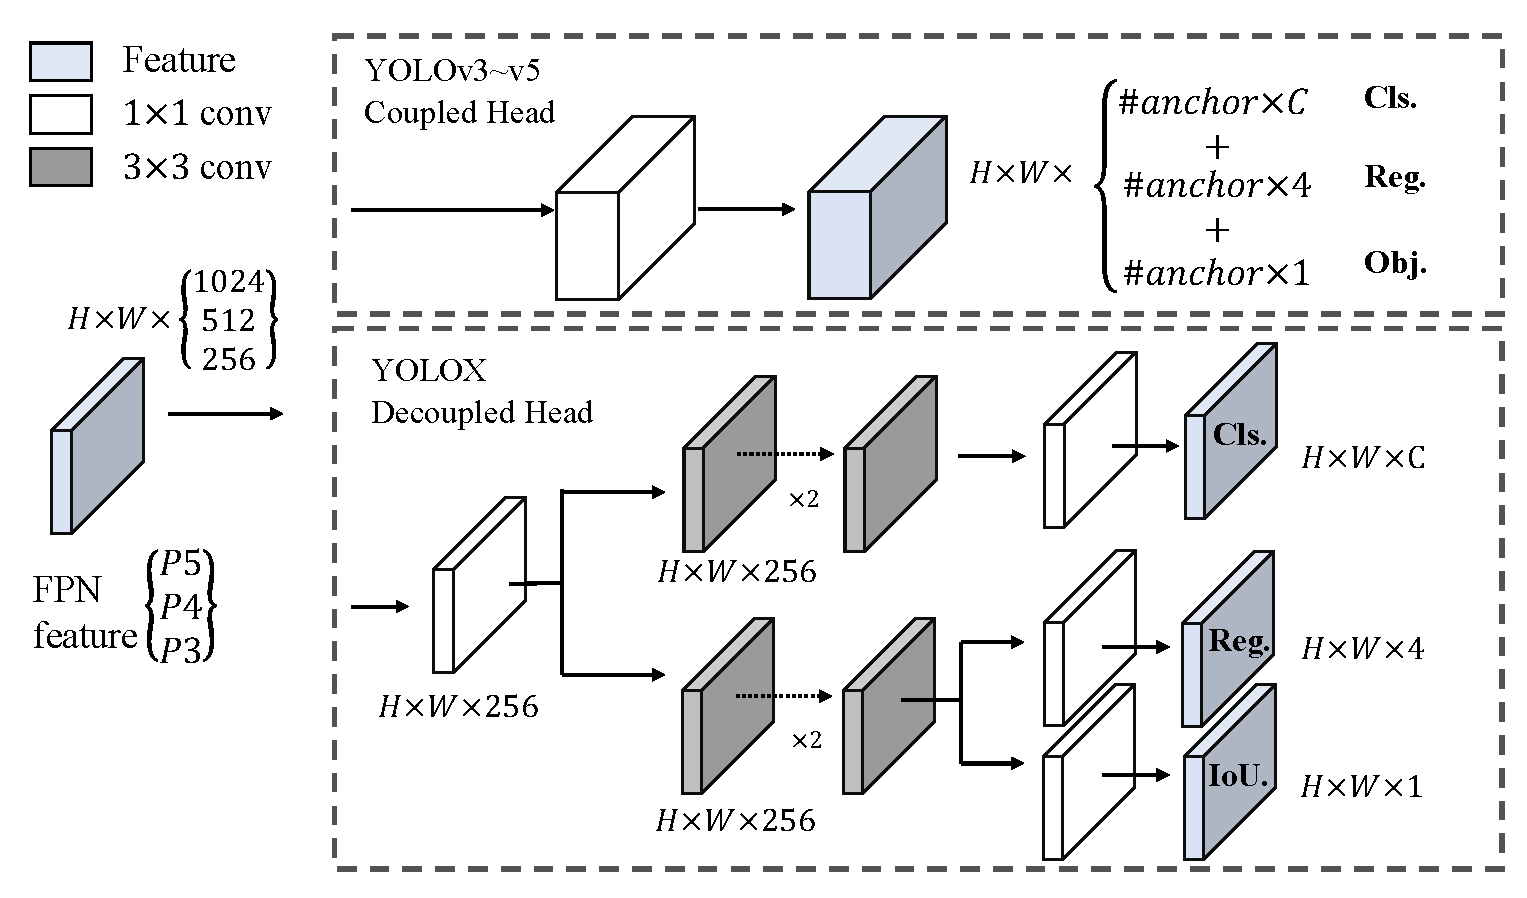
\includegraphics[width=\textwidth]{figures/related_work/yolox-graphic.pdf}
  \caption{Comparison between Yolo and YoloX \cite{yolox2021}. As mentioned, YoloX decouples its heads, allowing more accurate results for classification and bounding box detection.}
  \label{fig:yolox_multi_head}
  \clearpage
\end{figure}
% Own work
\chapter{Own Work}
\label{ch:ownwork}
\section{Stable Diffusion Pipeline}

One of the thesis's main goals was to build a diffusion-based pipeline to enhance synthetic tracking data like from the Synthehicle dataset \autoref{ch:synthehicle} and evaluate them afterward. This section will focus on the software engineering side behind the pipeline implementation, explaining core features and functionality.

\subsection{Programming language and project structure}

For the programming language, Python was chosen as it has great libraries for image parsing (\href{https://github.com/python-pillow/Pillow}{"Pillow"}) and the \href{https://github.com/huggingface/diffusers}{"diffusers" package}, which allows fast integration of various hugging face models, especially in the Stable Diffusion space. Also, one of the core modules, ALDM \cite{li2024aldm}, is also mostly written in Python, which makes integrating this project into the pipeline much easier.

Python allows the split of the project into multiple packages \autoref{fig:package_diagram_sd_pipeline}, which later could be distributed easily via \href{https://conda-forge.org/}{Conda-Forge} or \href{https://pypi.org/}{PyPi}. Therefore, the pipeline is structured in a highly modular way, ensuring easy extendability while keeping installation requirements minimal. Each module is currently maintained within a mono repository, managed by \href{https://github.com/pdm-project/pdm}{"PDM"} which is installed on top of a  \href{https://docs.anaconda.com/miniconda/}{"Conda"} environment. This unconventional package management approach offers three main advantages:

First, Conda enables the installation of packages from Conda Forge and binaries, which is particularly beneficial for optimized, platform-specific package builds.

Second, PDM assists in managing dependencies through its lock file and mono repository support.

Third, this unconventional approach allows for the installation of packages before the PDM install, facilitating the resolution of package dependencies such as \href{https://github.com/pytorch/pytorch}{PyTorch} to compile instructions from YoloX.

\begin{figure}[H]
  \centering
  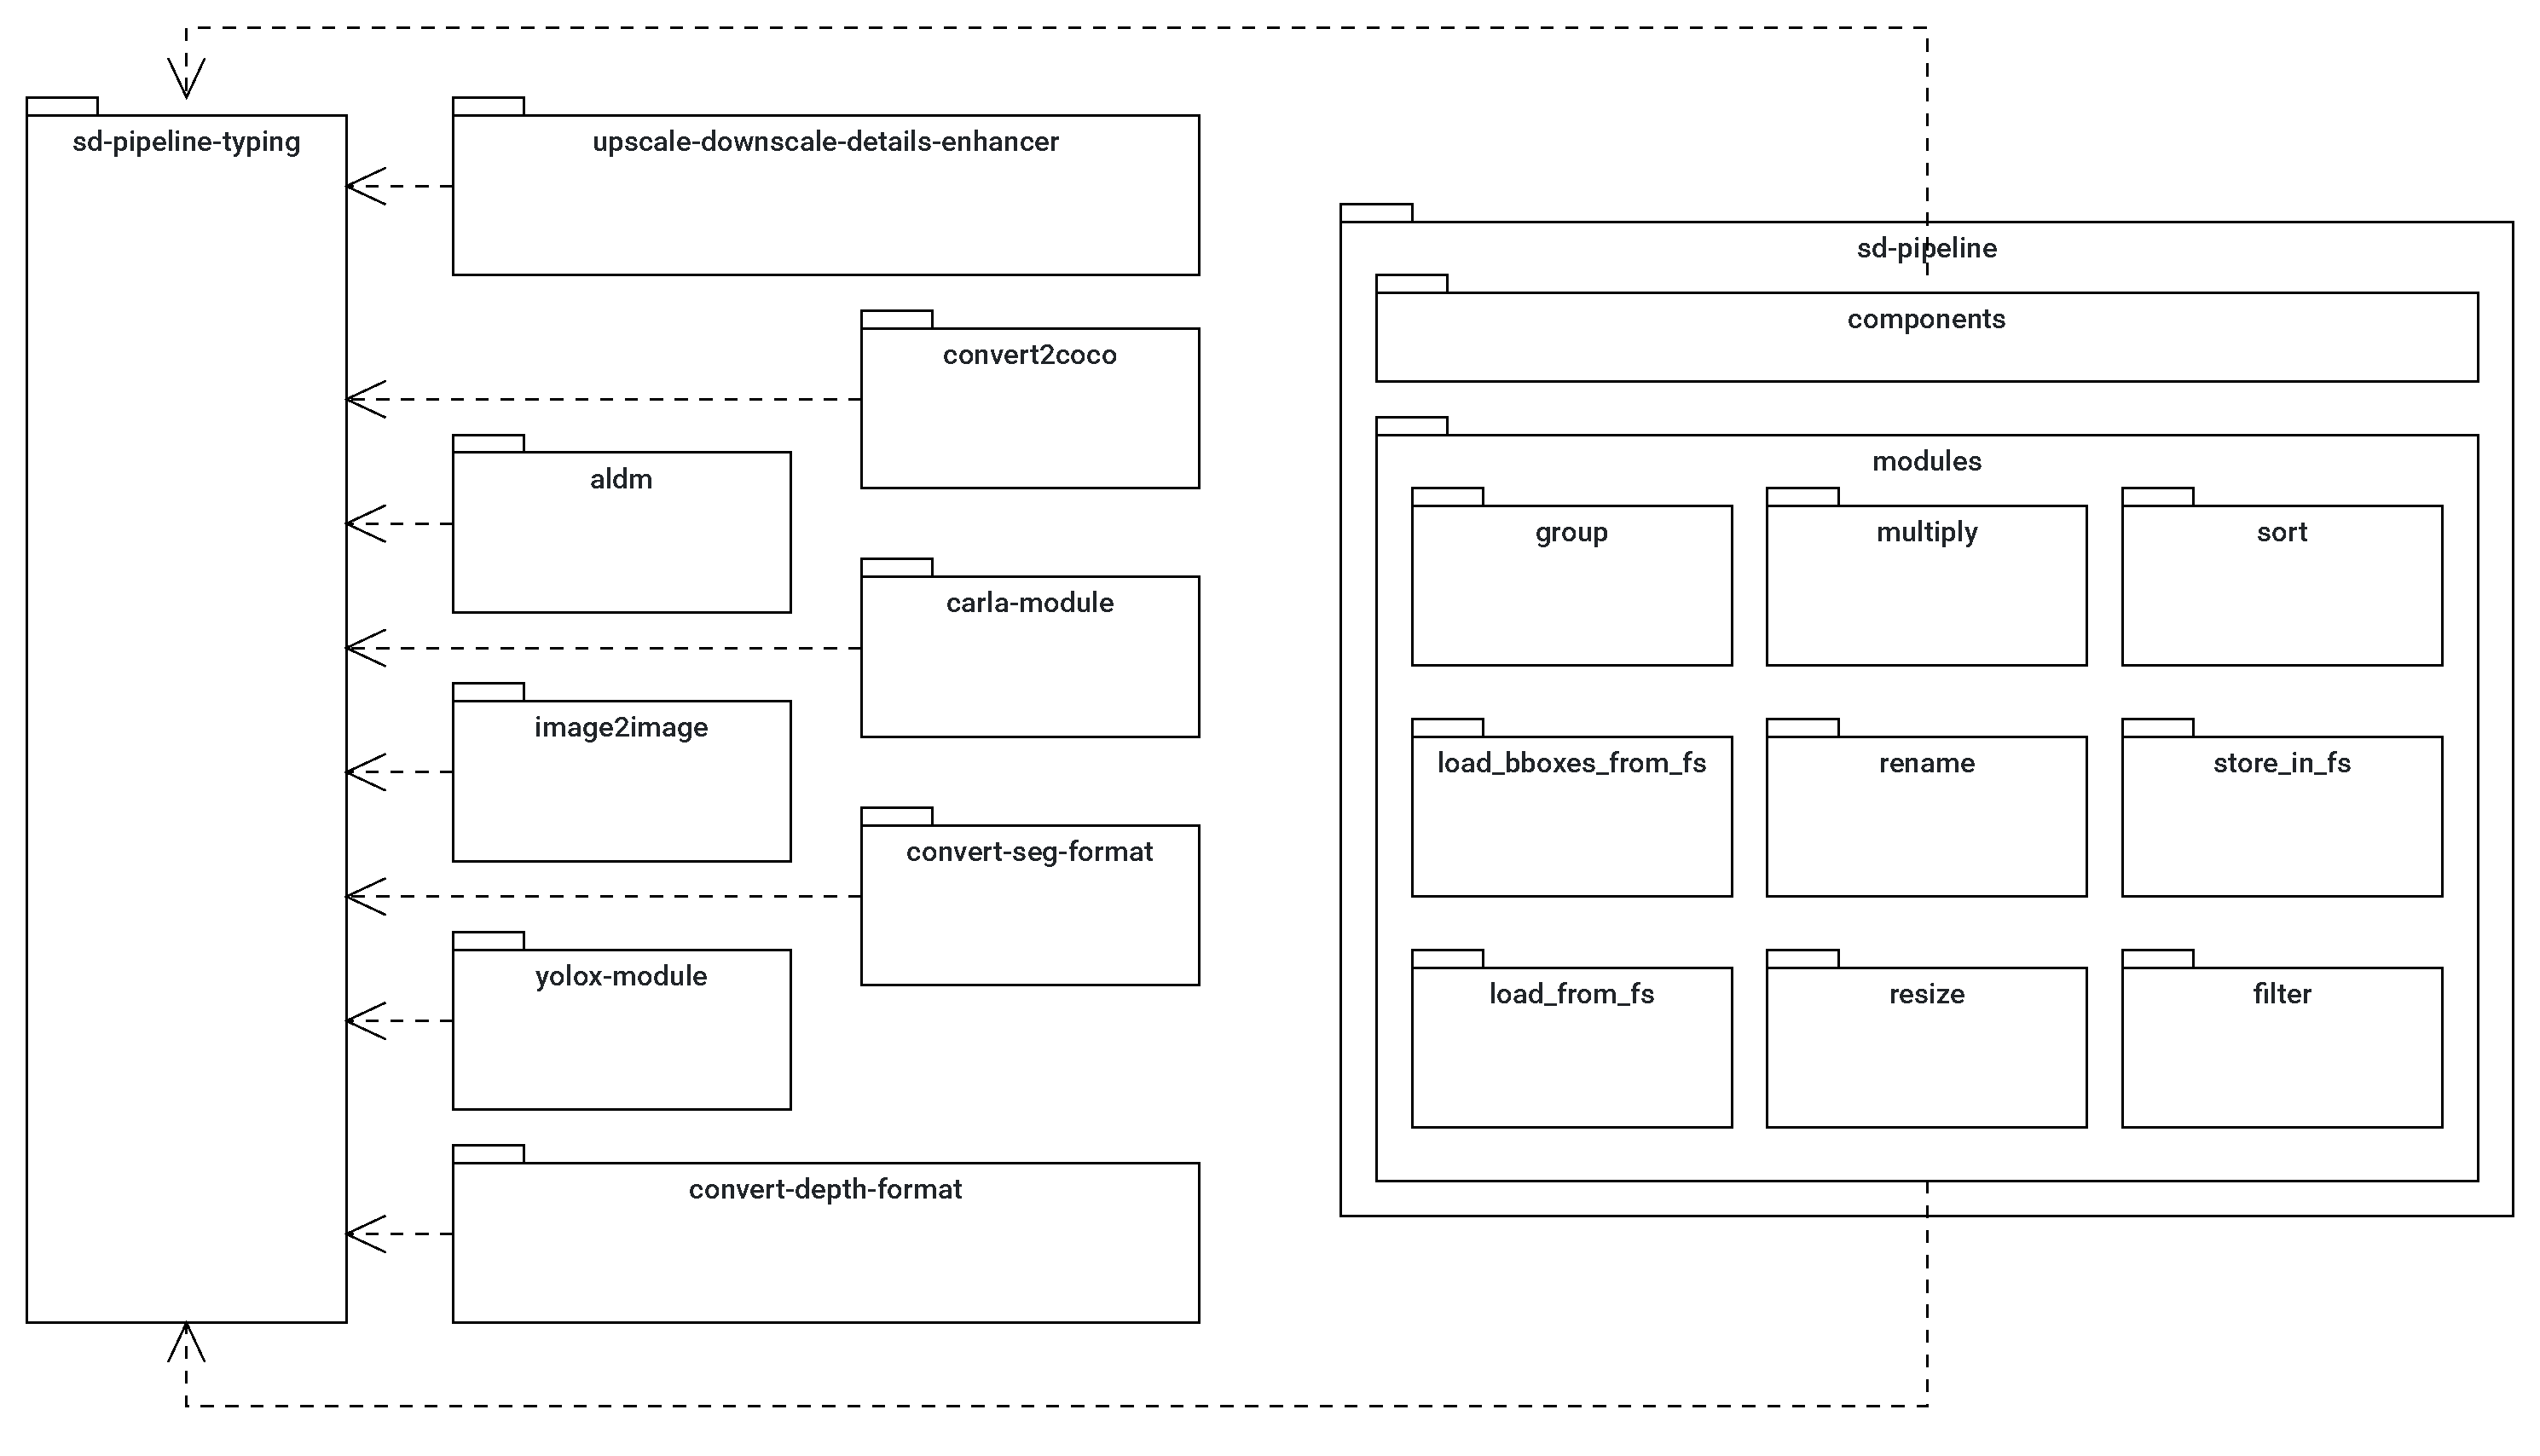
\includegraphics[width=\textwidth]{figures/own_work/pipeline/package_diagram.pdf}
  \caption{Package Diagram for the implemented modules}
  \label{fig:package_diagram_sd_pipeline}
  \clearpage
\end{figure}

\subsection{Dataflow and Stream Structure}

Each function that is encapsulated in different pipeline methods accesses the pipeline's data stream. The data stream contains the image that should be processed, metadata, and other information, like bounding boxes or depth information. The implementation of the stream allows three data types: 
    
\begin{figure}[H]
\begin{lstlisting}[language=Python]
      stream:   Dict[str, str | PIL.Image] |
                Tuple[Dict[str, str | PIL.Image]] | 
                None
\end{lstlisting}
\caption{Stream Data Type (The type should be \textit{PIL.Image.Image}, but due to its length, it will be abbreviated to \textit{PIL.Image} throughout the rest of this thesis.}
\end{figure}

The dictionary is the fundamental structure that contains all the important information for an image. In this context, the "Tuple" datatype was chosen as the container for managing multiple images or inputs in one stream. Tuples were selected over lists to highlight the importance of order within the stream and to emphasize the functional concept of immutable variables.


\subsection{Functionality}
\label{subch:functionality}

The \textbf{Pipeline} class is the heart piece of the application and contains all functions for building and executing different image processing pipelines \autoref{fig:class_diagram_sd_pipeline}. The implementation mostly follows the builder pattern \cite{10.5555/186897} by building the pipeline with different methods and getting the result after executing the run method. Therefore, a pipeline is represented through class methods that are chained together, with each method describing a step in the pipeline. Each of them returns the class object itself with a modified state by adding a function to its function array. All functions are executed in the end by the \textit{run} method. 

The \textbf{SubPipeline} class is a wrapper class around the "private" constructor of the Pipeline class (Python does not allow private constructors and does not have any equivalent to C++ friend classes. The underlying implementation, therefore, does not forbid access to the constructor from outside of the Pipeline class) and returns an empty Pipeline. This class should be used to initialize SubPipelines for different Pipeline methods.

\begin{figure}[H]
  \centering
  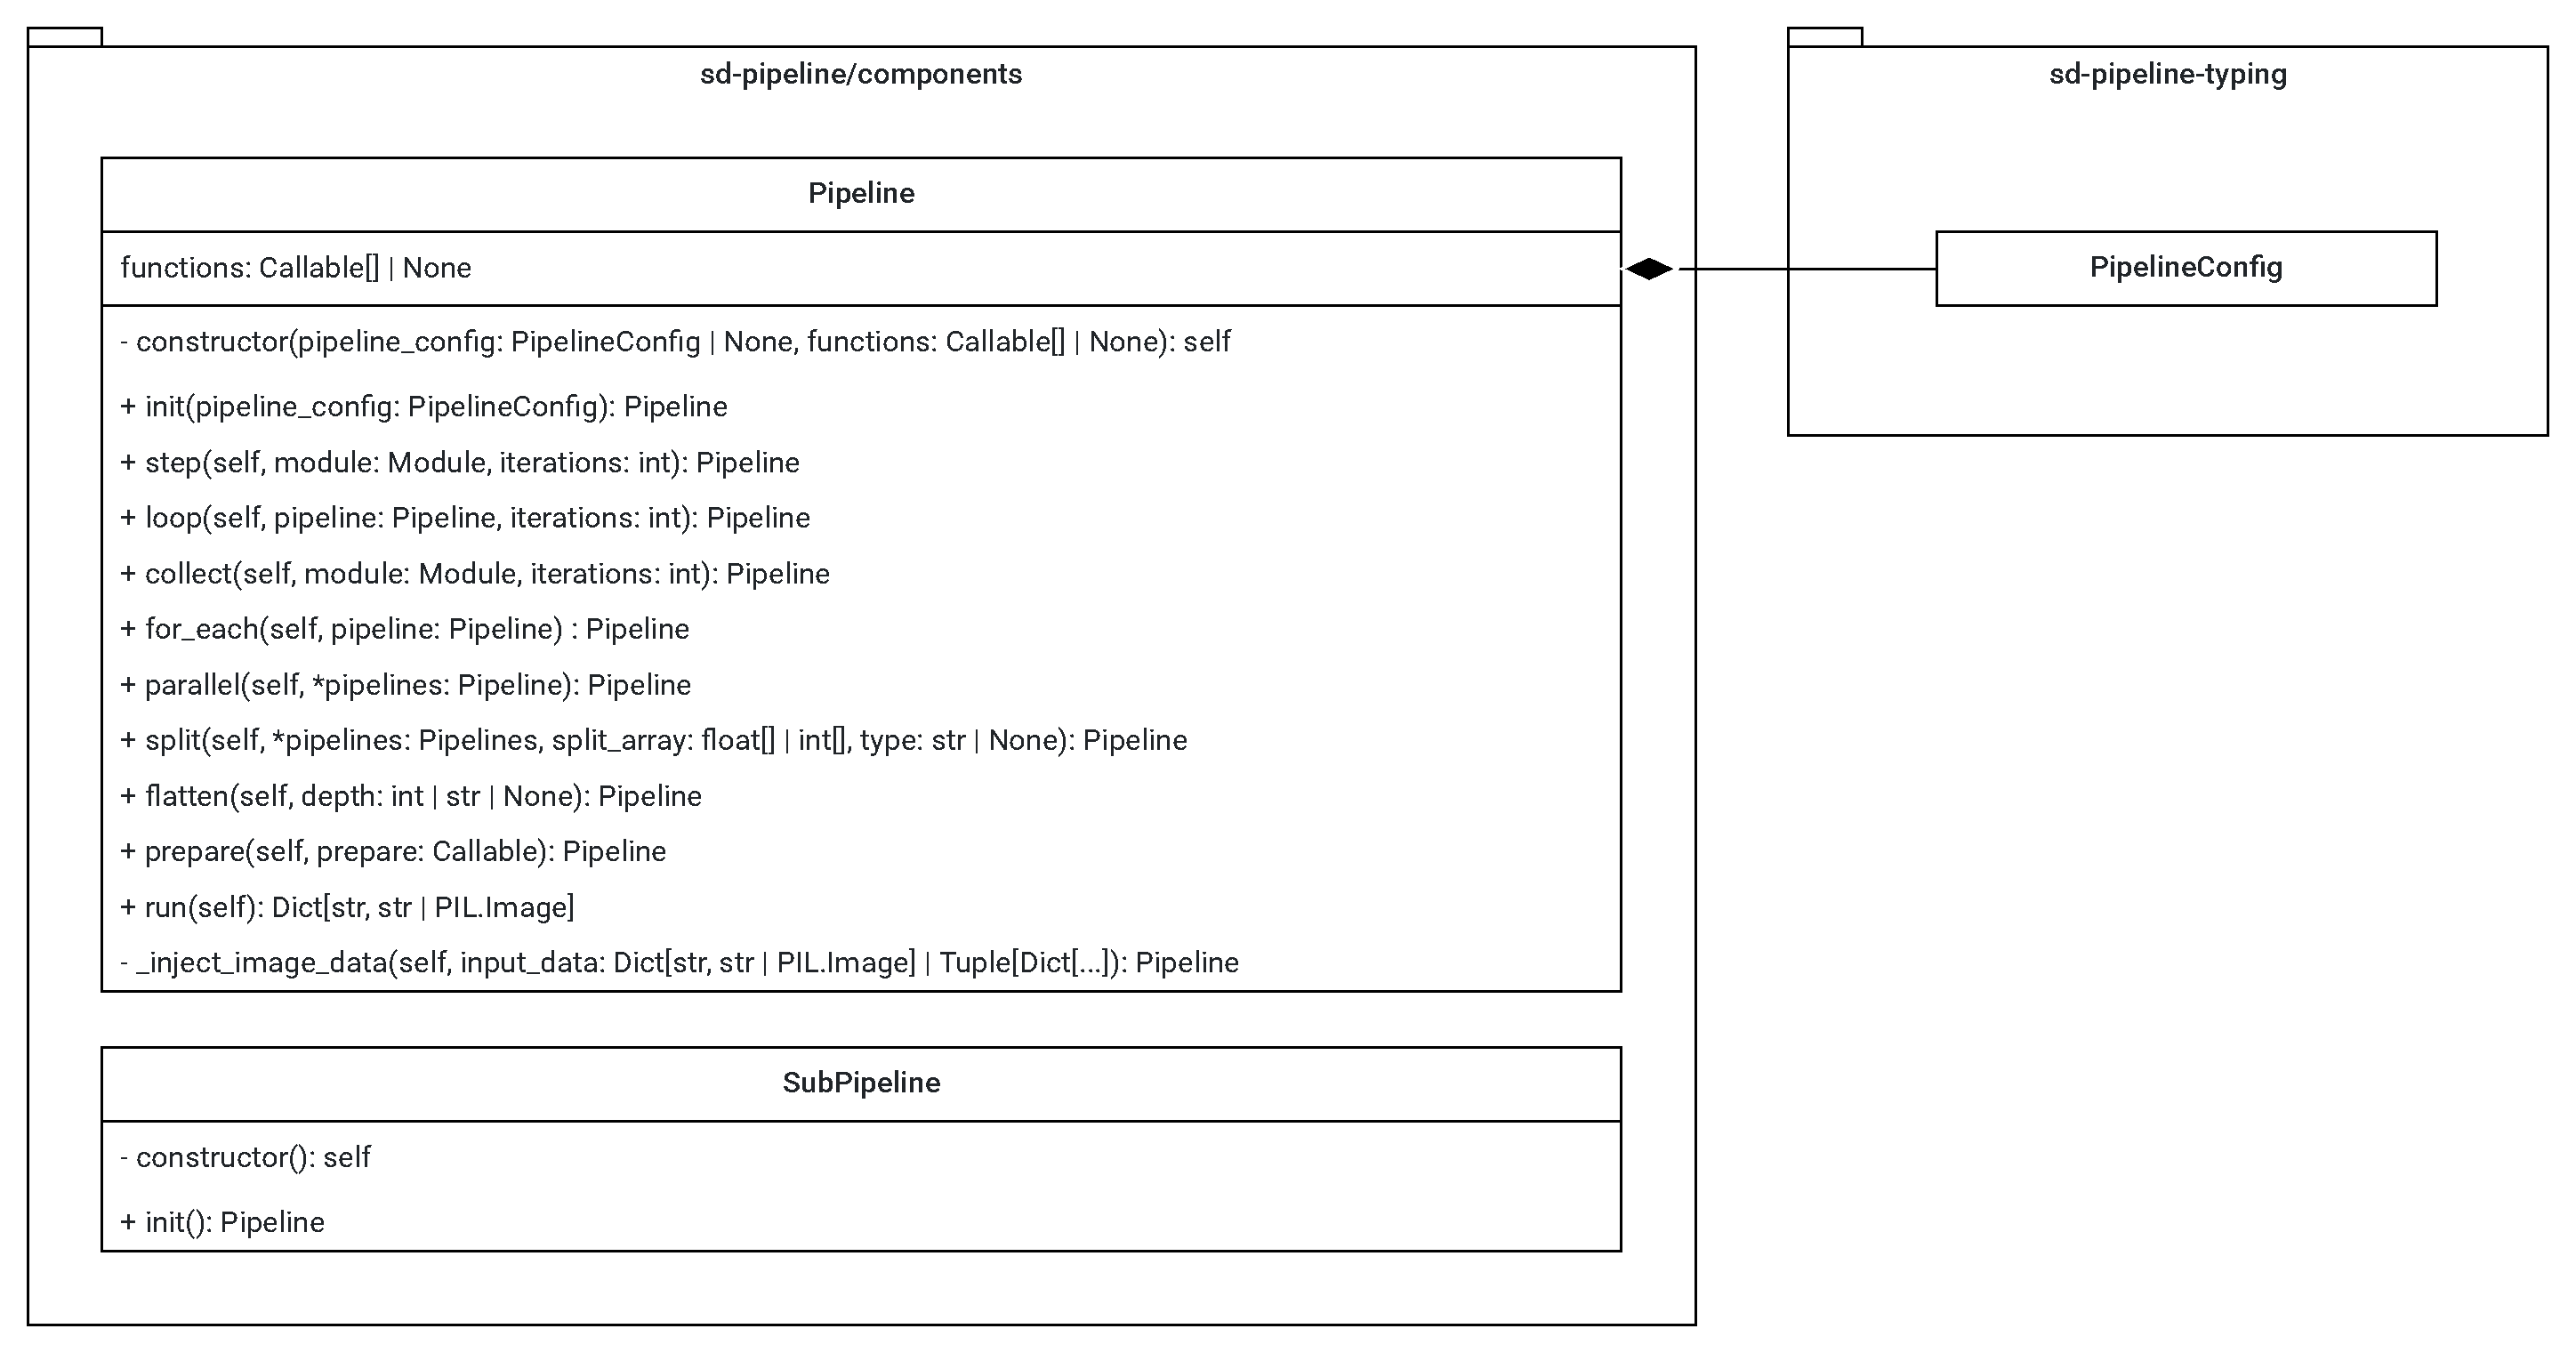
\includegraphics[width=\textwidth]{figures/own_work/pipeline/class_diagram_sd-pipeline_components.pdf}
  \caption{Class Diagram for the pipeline component (functions with the self attribute are class methods, otherwise they are static methods)}
  \label{fig:class_diagram_sd_pipeline}
  \clearpage
\end{figure}


To provide a large amount of functionality, the pipeline offers different methods to manipulate the stream of data that is pushed from function to function.

\begin{itemize}
    \item \textit{init()}: The init method is the only static function of the pipeline class and allows the initialization of an empty Pipeline. It helps with the injection of a pipeline config that is injected into each module \ref{sec:modules},

    \item \textit{loop()}: The loop method allows the execution of its SubPipeline for a defined amount of time. The output of the SubPipeline is the input for the next iteration.

    \item \textit{collect()}: The collect method also allows the execution of its SubPipeline within a defined amount of time. Here, each iteration gets the same input, and the results are returned in a tuple of tuples or dictionaries.

    \item \textit{for\_each()}: The for\_each method is often combined with the step method if specific modules can only have one image dictionary as its input. The method allows the execution of a given SubPipeline for each element in a Tuple.

    \item \textit{parallel()}: The parallel method runs multiple pipelines parallel with the same input and stores its output in a tuple (the functions inside the function array are still called sequentially - the reason for that is the Graphic card storage that would be a bottleneck for most computers).

    \item \textit{split()}: The split method splits its input stream into different output streams, each going into a separate SubPipeline. The ratio can be defined in absolute numbers or percentages.

    \item \textit{flatten()}: The flatten method flattens the output streams by unpacking tuples for positive depth parameters. For negative depth parameters, it's the other way around; the input is wrapped in tuples.

    \item \textit{run()}: The run method is the final step of building a pipeline. This method iterates over the statement array and calls the different functions added by all methods before.

    \item \textit{\_inject\_image\_data()}: This method manipulates the image stream by inserting new image data into it. Mostly, it is only used by other functions to copy a stream into a SubPipeline.

\end{itemize}

The last two functions that are not explained in this section, \textit{step()} and \textit{prepare()}, will be part of the next section, which focuses on exploring the module architecture.

\section{Modules}
\label{sec:modules}

Modules contain the main logic of the Pipeline and support one specific feature. Every module's structure is defined by the module superclass, which is part of the "sd-pipeline-typing" package, also displayed in \autoref{fig:package_diagram_sd_pipeline}. Modules are differentiated into base modules, all modules implemented inside the sd-pipeline package, and package modules, where each package contains a different module. The base modules contain relevant IO features or easy formatting features, while the package modules contain larger features like complicated mapping tasks or difficult-based transformations.
\begin{figure}[H]
  \centering
  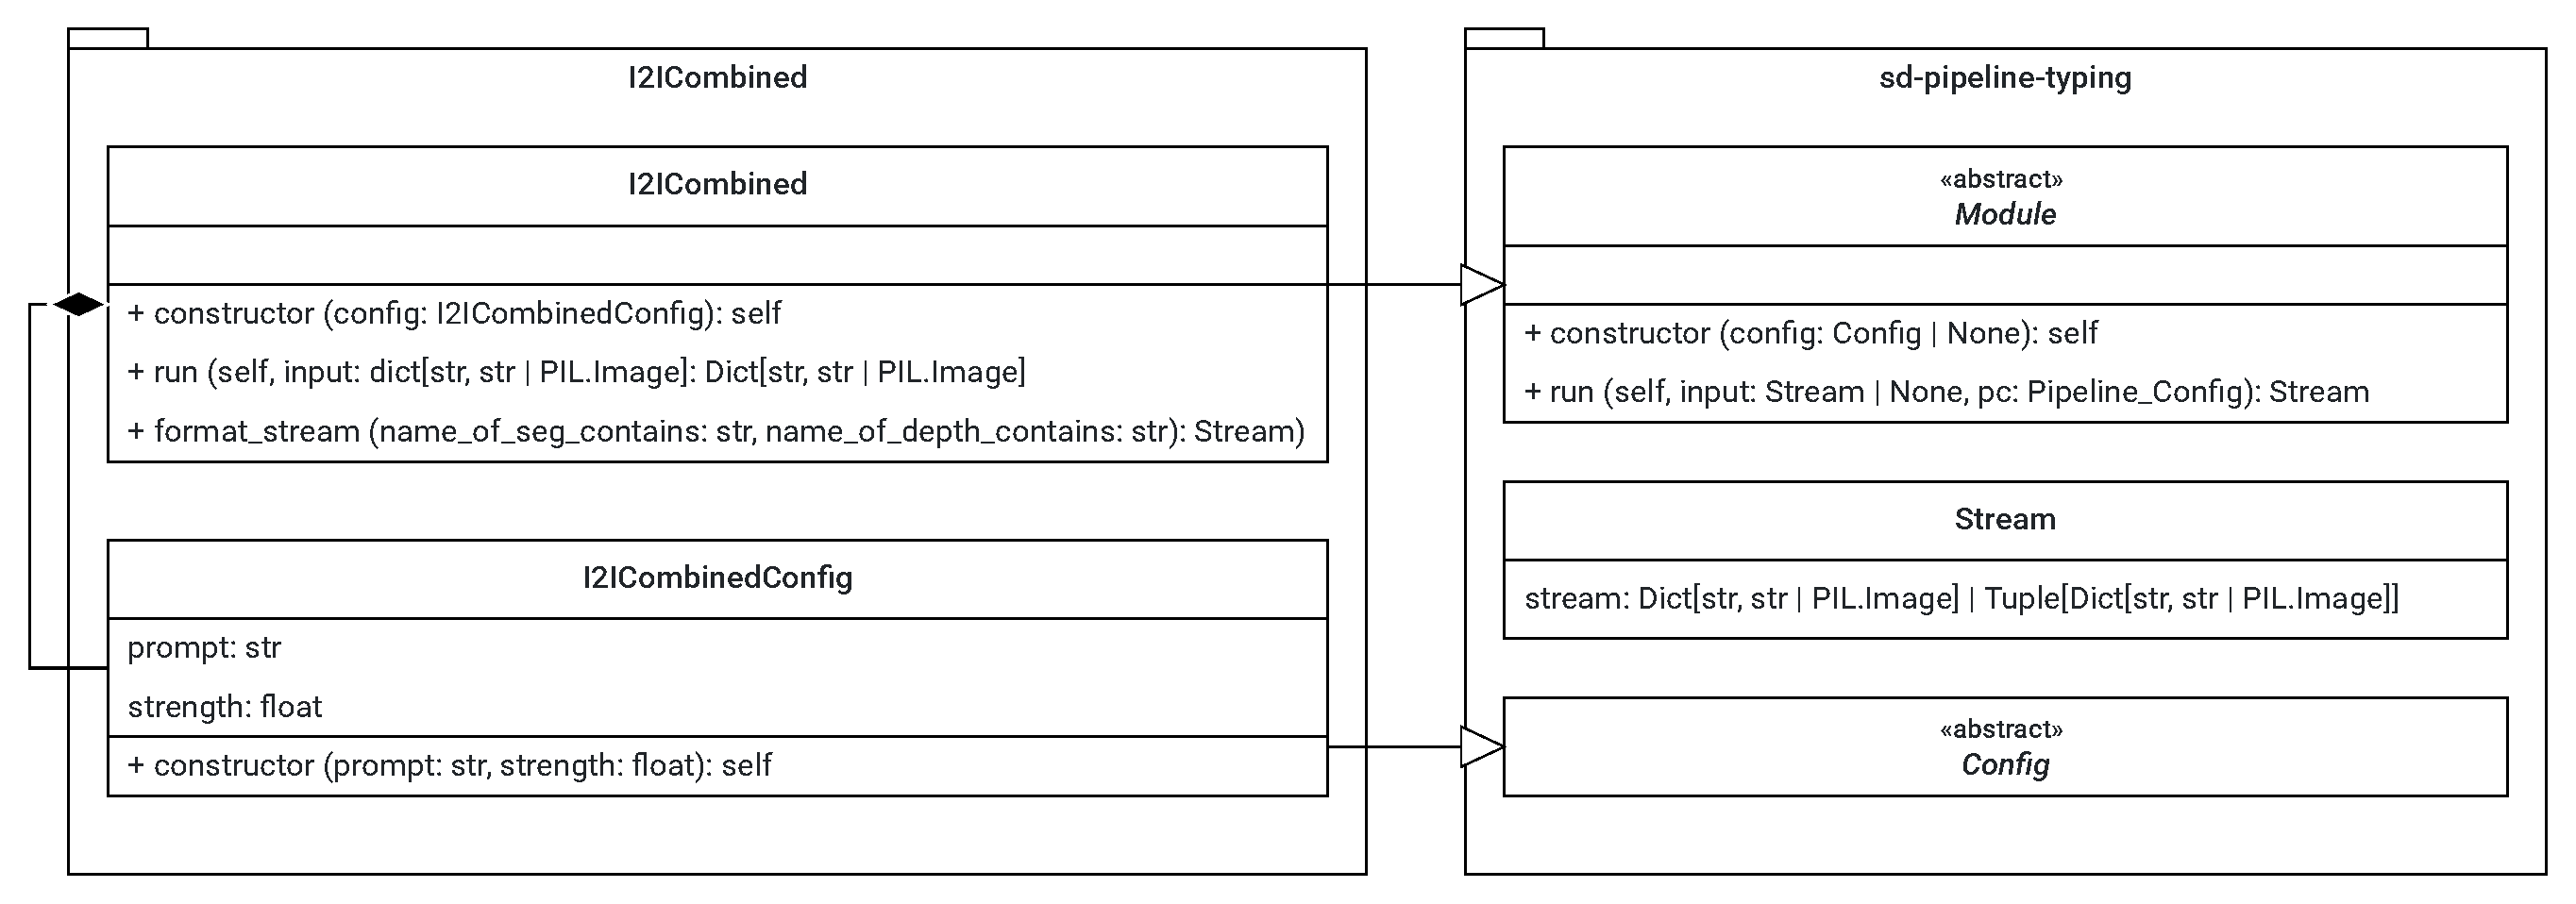
\includegraphics[width=\textwidth]{figures/own_work/pipeline/class_diagram_modules.pdf}
  \caption{Class Diagram describing the module architecture}
  \label{fig:class_diagram_module}
  \clearpage
\end{figure}

The module's interface is defined by two methods: the constructor, which initializes the module with the configuration object during pipeline programming, and the run method, which manipulates the data stream. This interface is established through the abstract class Module in the "sd-pipeline-typing" module. Additionally, the interface for configuration classes is provided within this package. All interfaces are implemented through inheritance, illustrated in \autoref{fig:class_diagram_module}.
Some modules also contain a static method named format\_stream for data stream manipulation, i.e. to assign segmentation or depth information to the appropriate images.

To integrate a module into the sd-pipeline, the \textit{prepare()} and \textit{step()} methods can be used. While the \textit{prepare()} method takes a callable as its only argument, allowing the format\_stream() method to gain access to the data stream, the \textit{step()} method takes a module as its parameter, adding the run method to the functions array and injecting the pipeline configuration. 

\subsection{Base Modules: pipeline-specific modules}

Some of the modules are directly implemented into the pipeline package. These modules contain core features and build the pipeline's data flow manipulation foundation. 
\\

The first and second ones are the I/O modules \textit{Load\_from\_fs} and \textit{Store\_to\_fs}. They are responsible for loading images into the Pipeline via the library "Pillow" and storing them afterward.
\\

The third I/O module \textit{Load\_bboxes\_from\_fs} loads bounding boxes from a JSON file into the pipeline stream, therefore providing metadata for the images that have to be matched with the help of other modules.
\\

\textit{Rename} and \textit{Resize} are two modules to manipulate an image by changing its name via a lambda function and resizing images with the help of the "Pillow" library. 
\\

The last four modules \textit{Group}, \textit{Multiply}, \textit{Sort}, and \textit{Filter} focus on manipulating not the images of the stream directly but changing the stream's behavior. \textit{Sort} sorts the dictionaries inside a stream by a given key, \textit{multiply} multiplies each dictionary by a defined number and \textit{group} groups $n$ streams together by combining all dictionaries from the same positions into a new tuple and filter removes image dictionaries that fail a predicate function.
\\

\subsection{Package Modules}

The package modules can be installed separately, and they are the main processing units of the pipeline. Therefore, this thesis will explain each of these modules in detail, also providing examples for the generated images and comparisons with a focus on object detection in \autoref{ch:evaluation}.
\subsubsection{CARLA}

\begin{figure}[H]
  \centering
  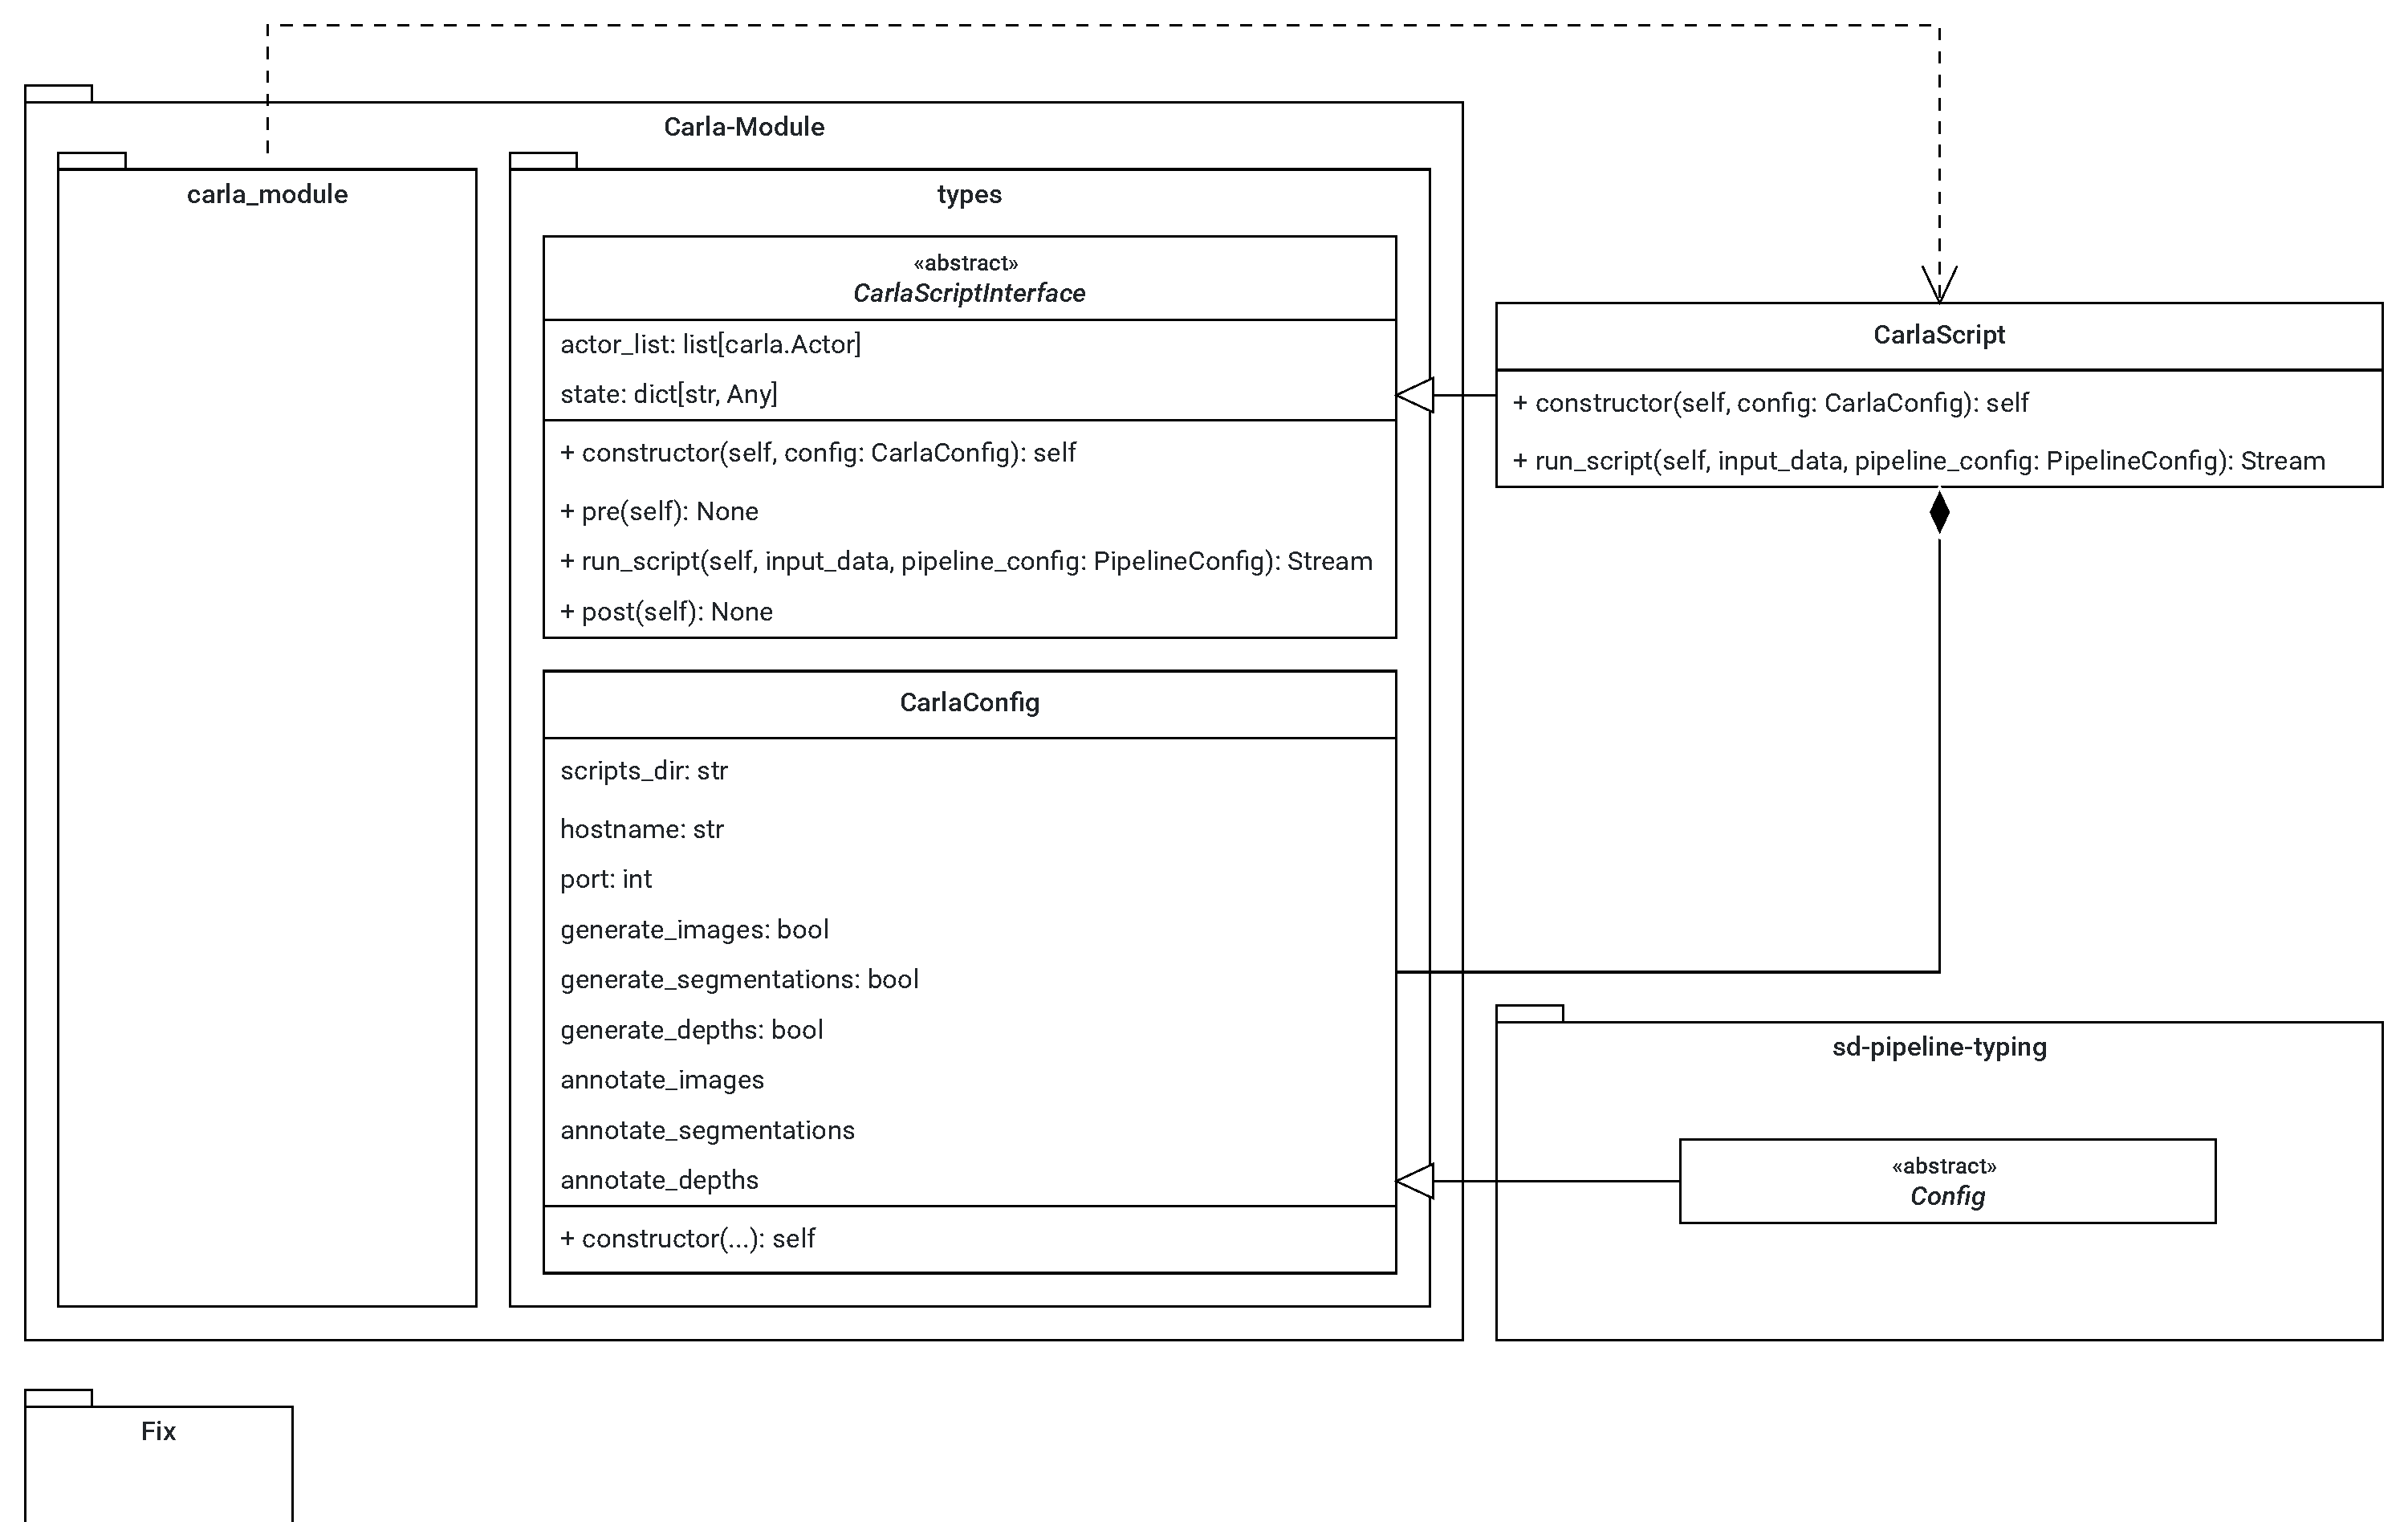
\includegraphics[clip, trim=0cm 3cm 0cm 0cm,width=\textwidth]{figures/own_work/modules/class_diagram_carla_module.pdf}
  \caption{Class Diagram describing the Carla script import architecture. The Carla module package is here presented as a black box. For more detail on how modules are structured, refer to \autoref{fig:class_diagram_module}}
  \label{fig:class_diagram_module_carla}
  \clearpage
\end{figure}

The CARLA module is logically the first module and facilitates data extraction from the CARLA Simulator (see \autoref{ch:carla}). Using the \href{https://pypi.org/project/carla/}{CARLA Python package}, it is possible to configure CARLA's simulation and export data such as semantic segmentation, depth information, and bounding boxes. To provide the pipeline user with complete flexibility for configuration, the module allows the loading of custom scripts called "Carla Scripts." These scripts are used to program the simulation. The interface "CarlaScriptInterface" is provided to help the user maintain the necessary structure (see \autoref{fig:class_diagram_module_carla}).

The module provides the functions \textit{pre()} and \textit{post()}, which are called before and after the \textit{run\_script()} function to set up the basic environment and clean up. The \textit{run\_script()} method itself is called from the carla\_module during the pipeline run, executing the script. 

Safety is a crucial topic, and it is important to acknowledge that this module should not be used in a public environment. The "Carla Scripts" are loaded without validation, which could allow malicious code to be executed during a pipeline run.

\subsubsection{ALDM}

ALDM (see \autoref{ch:aldm}) is the first step of the image generation process, allowing a segmentation map to be transformed into a realistic, detailed image with the help of a Stable Diffusion algorithm and a control net. To integrate the code into the pipeline, it had first been made installable as a package. Therefore, rewriting the original ALDM code and creating a wrapper around it to be called from my pipeline was necessary. Additionally, the configuration settings are extracted into a configuration class to make them accessible at the pipeline programming level.

\subsubsection{Image2Image}

The Image2Image module extends the ALDM processing by enabling further image manipulation after its initial creation. As described in \autoref{ch:controlnet}, image-to-image processes take an existing image as their base and generate a new one from it. This generation can be guided by ControlNets. This module implements multiple variations, including image-to-image without a ControlNet, the ControlNet trained on semantic segmentation by Lvmin Zhang \cite{zhang2023addingconditionalcontroltexttoimage}, the ControlNet trained on depth by Lvmin Zhang \cite{zhang2023addingconditionalcontroltexttoimage}, and a combination of both. All modules work with Stable Diffusion 1.5 \cite{rombach2022highresolution} as it was the only available Stable Diffusion checkpoint with a ControlNet trained on both inputs.

\subsubsection{Convert Seg Format \& Convert Depth Format}
To provide correctly formatted segmentation and depth information for the ControlNets in the image2image module, the segmentation maps and depth maps must be properly modified.
The convert-seg-format module offers methods to transform a semantic segmentation map from the Cityscapes dataset \cite{cordts2016cityscapesdatasetsemanticurban} format to the ade20k dataset \cite{zhou2019semantic} format and vice versa. This is essential because Sythehicle \cite{Herzog_2023_WACV} provides and ALDM \cite{li2024aldm} consumes Cityscape-formatted segmentation maps, while the ControlNet requires ADE-formatted segmentation maps.
The convert-depth-format module provides two functionalities. The first one inverts the depth map (Sythehicle provides depth information with the nearest objects being the darkest, while the depth control net requires the reverse), and the second one includes a denormalizer that allows a function to run on each pixel of a depth map, reverting possible normalizations.

\subsubsection{Upscale-Downscale-Details-Enhancer}

The upscale downscale module tries to enrich image data with more details by first up-scaling the image with the help of a latent diffusion network \cite{rombach2022highresolution} and then down-scaling it with "Pillow". This should help with missing details and broken proportions by adding/repairing them during the upscale process and not losing them completely during the downscale. In combination with the loop method provided by the pipeline, which can be found in \autoref{subch:functionality}, this module could enhance the image multiple times before passing it to the next pipeline method. Its idea originates from the DLSS-Algorithm developed by NVIDIA \cite{watson2020deeplearningtechniquessuperresolution} for PC-Games, which also takes a low-resolution image, upscales, and afterward downscales it to the monitor resolution to provide better image quality.

\subsubsection{Convert to COCO}

As the package name already states, this module converts an input stream into the COCO format \cite{lin2015microsoftcococommonobjects}, exporting the label files as JSON. With the help of the \textit{split()} method, \autoref{subch:functionality}, and some prepossessing functions, the input stream can be split to allow the dataset to contain the train, test, and validation labels. The purpose of this module is primarily to help with the evaluation through the \textit{yolox} module.

\subsubsection{YoloX}
The YoloX module is the main evaluator module providing object detection on COCO datasets \cite{lin2015microsoftcococommonobjects}. YoloX provides different models with different layer sizes, offering  large flexibility for training. The module wraps the \href{https://github.com/Megvii-BaseDetection/YOLOX}{YoloX package} \cite{yolox2021}, allowing it to be integrated into pipelines seamlessly.

\subsubsection{Finetuning}
A key feature of YoloX is the ease with which the model can be trained or fine-tuned. The pipeline is designed to facilitate the fine-tuning of existing checkpoints using newly generated data, ensuring that the model can be enhanced by that.

\subsubsection{Resulting checkpoints and evaluation}
After every epoch, YoloX provides a new checkpoint with the updated weights and training results consisting of the precision and recall values for each class. The module also exports them, providing the possibility to compare different pipeline configurations and use the trained checkpoint for other projects \autoref{ch:evaluation}.

\section{Visual and Object detection testing}
Another part of this thesis is the evaluation of the different modules and a detailed comparison between the results of different pipelines. Multiple tests regarding object detection have been run to test the performance and quality of the different results, and the output has been analyzed visually.

\subsection{Test setup}

For the major generation modules, small tests have been conducted to determine the best configurations. Following this, a dataset containing 300 segmentation maps was generated from six different settings within the Synthicle dataset (Town01-N-..., C01 - CO6, 50 segmentation maps from the selected scene) (\autoref{ch:synthehicle}) and the MUAD dataset (300 images out of the validation set, because annotations for the test set was not available) (\autoref{ch:muad}). Four main themes, daytime, dawn, rain, and night were applied to the  300 segmentation maps, resulting in 1,200 images. This process was repeated twice, ultimately producing 2 datasets, each containing a total of 2,400 finalized images.

Due to time constraints (the generation for every dataset took over 3 days), the images from other datasets were used as a base for new ones. For example, when using the image2image module, the output from the ALDM Module was taken as the new input instead of regenerating the images resulting from the ALDM modules. While this could carry graphical errors through the tests, new generations could also introduce new graphical errors, making this an efficient trade-off between time and dataset size.

The dataset generation and the later conducted tests run on two machines, with the first one having two NVIDIA Titans and the other one having an NVIDIA RTX 4070. On both machines, the tests were run with the same YoloX settings.

\subsubsection{Object detection with pre-trained model}

With the resulting images, object detection for the train images was conducted to measure the quality of the different data sets by looking at the average precision (AP) and average recall (AR) the pre-trained COCO weights for the YoloX model can achieve (more details on these measurements in \autoref{sec:test_results_object_detection}). 

\subsubsection{Object detection model finetuning}

With the resulting datasets, the YoloX reconfigured COCO weights were further fine-tuned and evaluated with 600 random images from the Cityscapes dataset to test if the module could be further optimized through data generated with a Stable Diffusion algorithm. As mentioned in \autoref{ch:cityscapes} the dataset was enhanced by adding foggy and rainy scenes to make detecting cars harder.

\section{Consistency and tracking testing}
Maintaining spatial and temporal consistency between different image generations is a problem most diffusion modules have. Four different test approaches were conducted to visualize the problem and test how spatial and temporal consistency could be preserved. For each test, the same six starting images were used.

\subsection{Test setup Baseline}
The Synthhicle dataset was used for these tests, as the images originate from videos and are, therefore, sequential. Per scene, 100 images were taken, and we are building the baseline for the other tests that will modify these images.

\subsection{Test setup ALDM}

This test focuses on generating 100 images with ALDM. The input was 100 segmentation maps that followed one another, resulting in a 10-second-long video with 10 frames per second.


\subsection{Test setup image to image, segmentation ControlNet}

\begin{figure}[H]
  \centering
  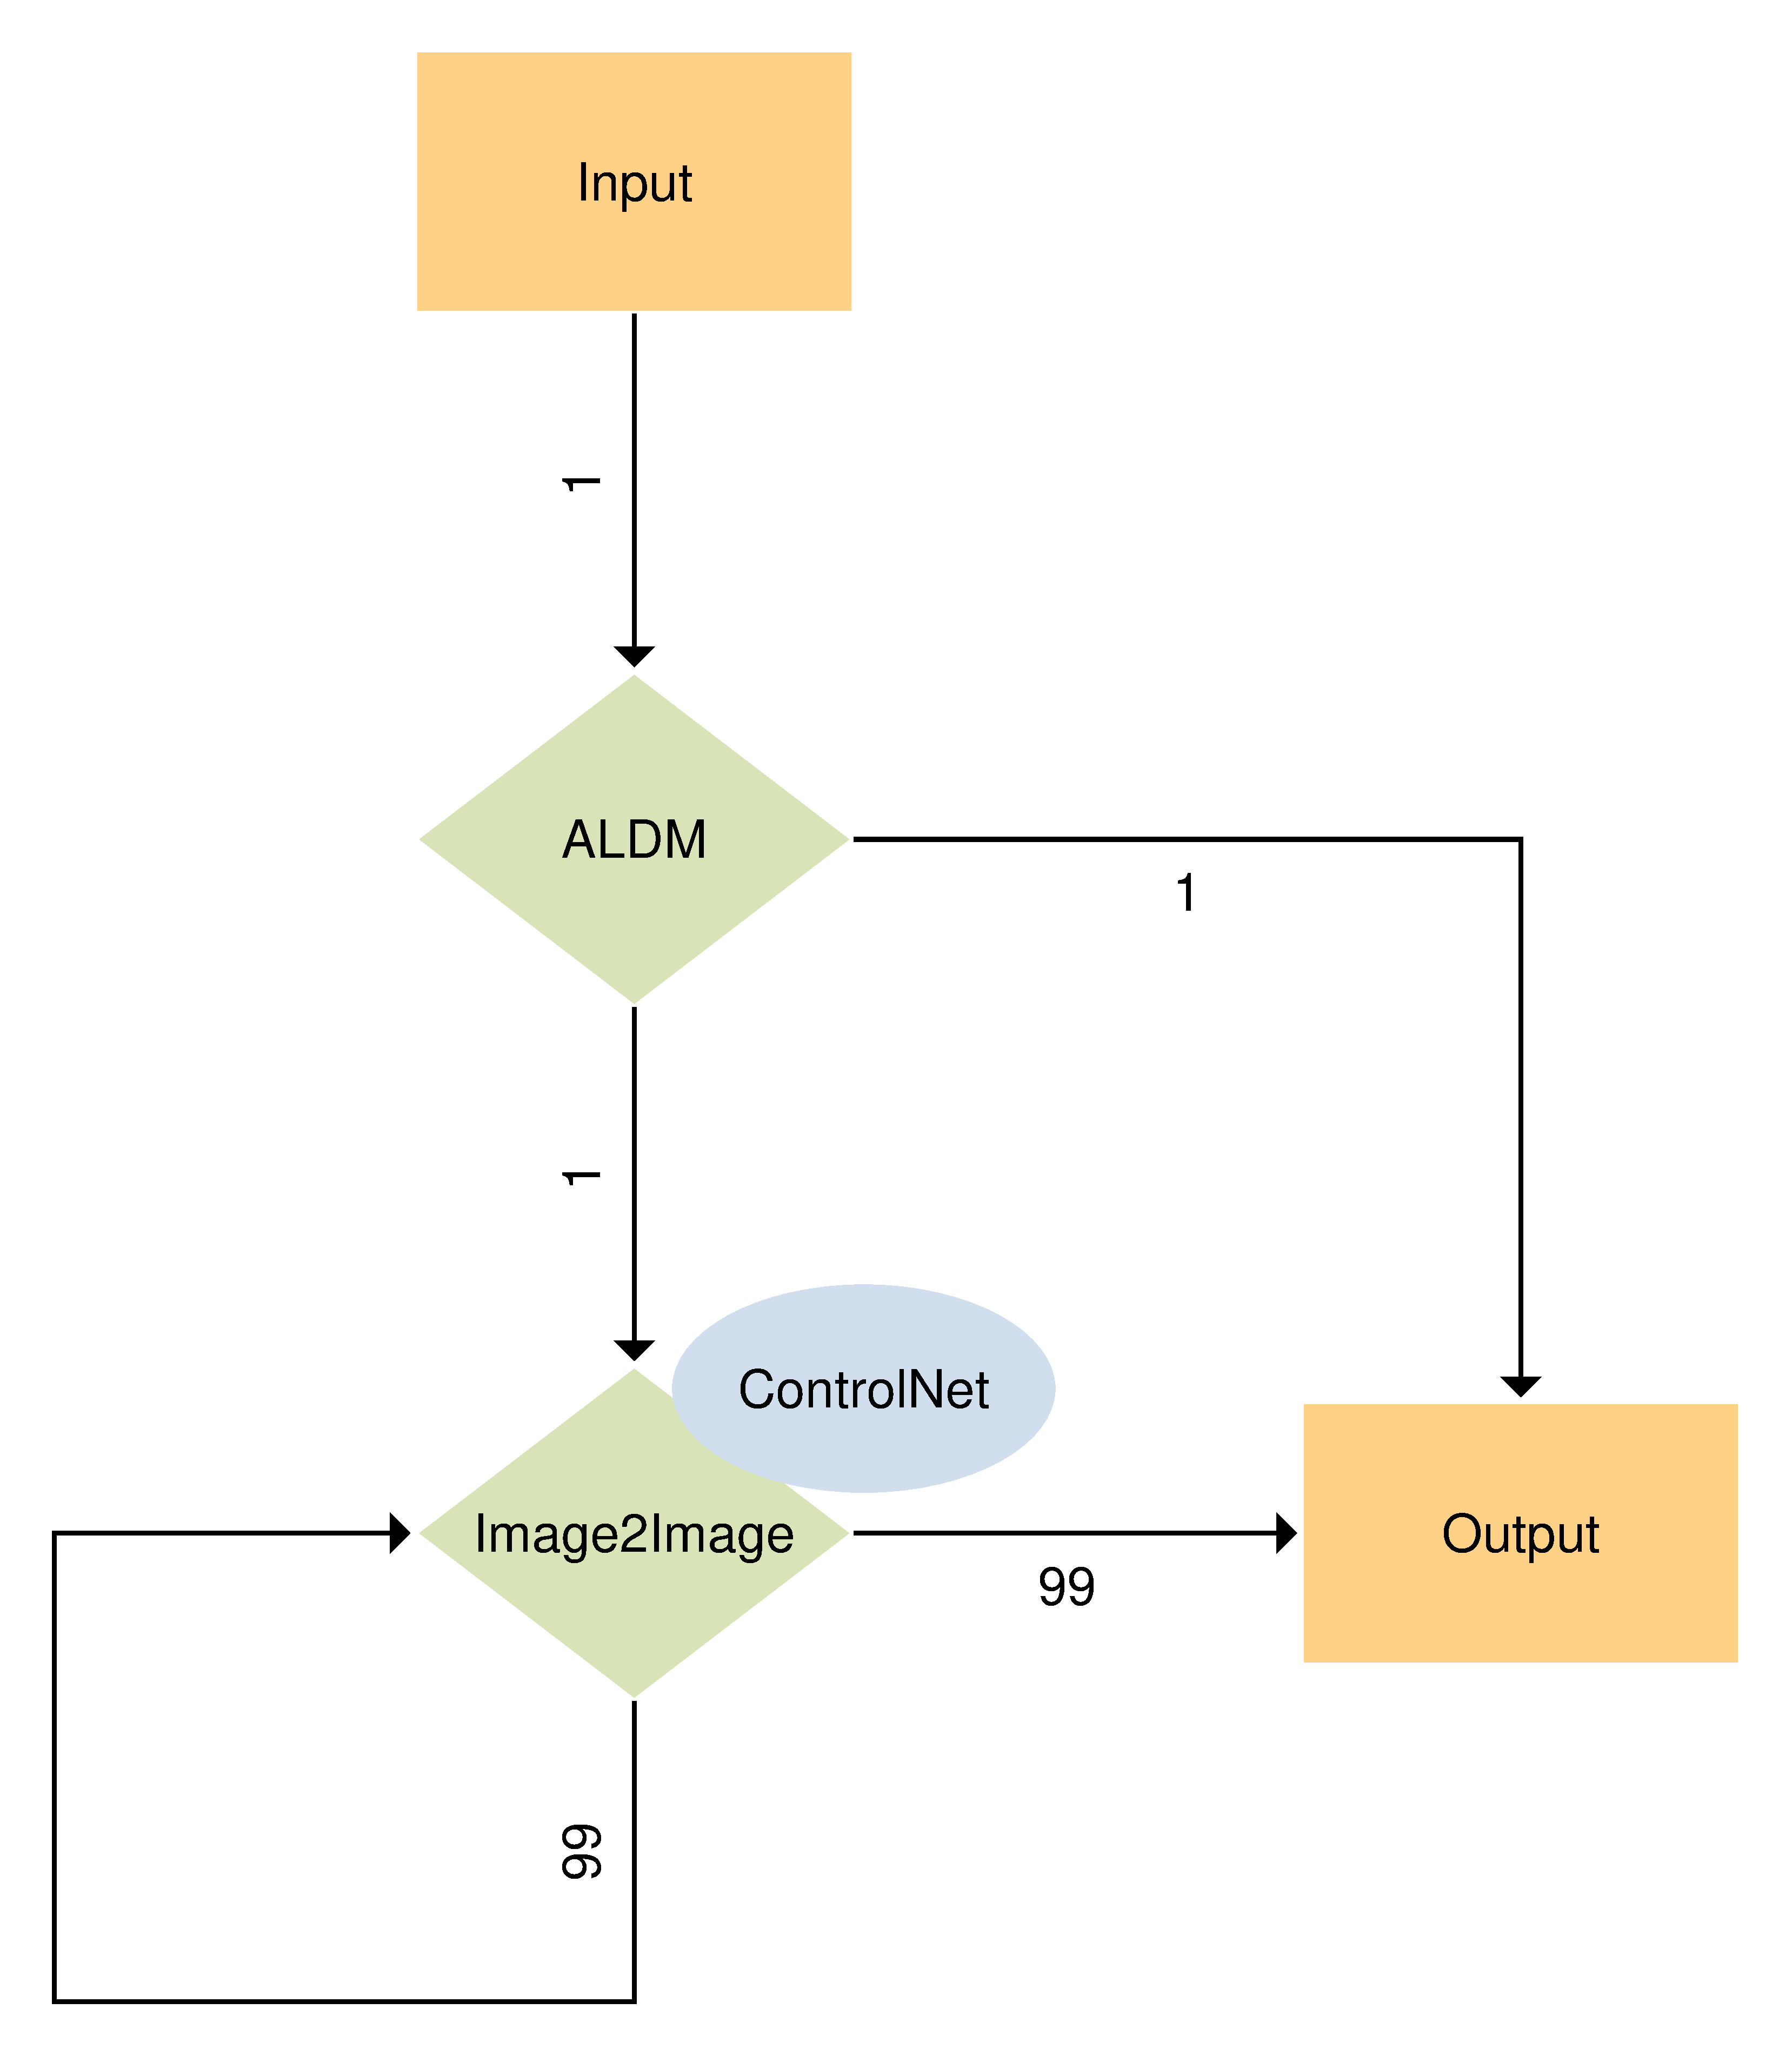
\includegraphics[width=0.5\textwidth]{figures/own_work/temporal_spacial_consistency/temporal_consistency_i2i_pipeline.pdf}
  \caption{Visitation of the i2i consistency pipeline}
  \label{fig:temporal_consistency_i2i_pipeline}
  \clearpage
\end{figure}

For the next test, as shown in \autoref{fig:temporal_consistency_i2i_pipeline}, only the first segmentation map is used as input for the ALDM module. The resulting image is the starting point for the image-to-image process, with every step generating a new frame with the previous output as its next input. To guide the generation for the following frame, the segmentation ControlNet is used together with the next fame segmentation map. The resulting video is 10 seconds long with 10 frames per second. During different tests, the prompt of the image-to-image module was changed to cover multiple scenarios. For the final result, the seed and the strength parameter were kept the same (see \autoref{sec:high_score_for_the_strength_parameter} and \autoref{sec:color_shifting_of_the_scenes} for more details).

\subsection{Test setup image-to-image, segmentation \& depth ControlNet}

This test has a similar test setup as the previous one, only differing in the used ControlNets, combining segmentation maps with depth information. 

\subsection{Image constancy evaluation}

To evaluate the consistency of these different videos, the previous image is compared to the current image via the Root Mean Square Error (RMSE; for calculation details, refer to the \href{https://github.com/up42/image-similarity-measures/blob/master/image_similarity_measures/quality_metrics.py}{used implementation}) to see how big the change between two consecutive frames is. This is compared to the synthetic image video (the baseline).


\subsection{Object tracking evaluation}

With the help of \href{https://github.com/ultralytics}{Ultralytics}, Bytetrack \cite{zhang2022bytetrackmultiobjecttrackingassociating}, and pertained Yolo v8 \cite{reis2024realtimeflyingobjectdetection} weights, every vehicle in the video was tracked during the 10 seconds and labeled with a unique ID. The IDs are assigned in ascending order, increasing by $1$ for each subsequent vehicle. If the tracking algorithm loses the car, a new ID is assigned. In the end, the difference between the number of IDs counted on the synthetic image video (the baseline) and the number of IDs is used as a metric for the quality of the generated cars and their stability between different frames.
% Results
\chapter{Evaluation}
\label{ch:evaluation}

\section{Object detection}

\subsection{Visual classification of the output images}
\label{sec:looking_at_the_output_images}

\begin{figure}[H]
  \centering
  \includegraphics[width=\textwidth]{figures/evaluation/elvaluation_images.pdf}
  \caption{Comparing the different results of the generation. From top row to bottom row: synthetic data from MUAD and Synthehicle, segmentation maps, Output ALDM, Output ALDM + I2I Seg, Output ALDM + I2I Seg + Depth}
  \label{fig:results_generation}
  \clearpage
\end{figure}

All generations often have problems finding the right car proportions, leading to curved edges and unnatural shapes. This happens especially with objects close to the camera, hinting that ALDM has not been trained in this type of situation. Looking at \autoref{fig:results_generation}, ALDM dominates the car generation, especially for the out-of-the-car view (from now on called first-person view), while for the top-street view (from now on called third-person view), Stable Diffusion 1.5 with the image-to-image module is able to correct the outline of cars and streets, especially if the cars are small. For closer cars,
details are lost because of the added noise from the Stable Diffusions image-to-image process, which is not completely removed. This is especially noticeable in the image-to-image generation with only segmentation maps. Adding depth maps and a slightly higher strength parameter (for more details, see \autoref{sec:high_score_for_the_strength_parameter}), which is possible due to the extra guidance through the depth maps, the noise can be heavily reduced, often resulting in random clouds in the image (see in \autoref{fig:results_generation}).

Stable Diffusion 1.5 with ControlNets really amplifies weather conditions and lighting. While ALDM's lighting and weather conditions are mostly slightly hinted at, ControlNet overdoes it sometimes, leading to a more interesting but less realistic image. Comparing images in \autoref{fig:weather_conditions}, one can spot the new lightning and reflection added by Stable Diffusion 1.5.

\begin{figure}[H]
  \centering
  \includegraphics[width=\textwidth]{figures/evaluation/evaluation_weather_effects_and_lighting.pdf}
  \caption{Looking at different prompts, Stable Diffusion 1.5 with segmentation and depth ControlNet (bottom) highlights and enhances the weather and lightning effects of ALDM (top)}
  \label{fig:weather_conditions}
  \clearpage
\end{figure}

\subsection{Test results object detection}
\label{sec:test_results_object_detection}

To evaluate test results for object detection, two matrices are highly important: the average precision (AP):
$$AP = \frac{\text{True Positive}}{\text{True Positive} + \text{False Positive}}$$
and the average recall (AR):
$$AR = \frac{\text{True Positive}}{\text{True Positive} + \text{False Negative}}$$
The average precision, which is the main metric used to evaluate performance in YoloX, shows the ratio of rightfully detected pixels for a class to all detected pixels. The average recall shows the ratio of how many pixels of one class were detected from all pixels that are part of the class.

\subsection{Test results object detection on train set}
\label{sec:test_results_object_detection_on_train_set}
Looking at \autoref{tab:results_yolox_object_detection}, the raw synthetic dataset has the highest AP of both datasets, resulting from better-defined car shapes and proportions compared to the diffusion approaches. ALDM I2I Seg + Depth outperforms the base ALDM and I2I Seg in MUAD and Synthehicle, especially regarding its AR, outperforming the pure synthetic data as well. Looking at the AP performance, the gain of image-to-image is much less for the first-person dataset because the images generated by ALDM already have better proportions there. This only results in more added noise by the image-to-image module, explaining the large gap in the raw synthetic data. Also, Synthehicle's data is much less detailed, giving another advantage to the diffusion approaches and resulting in closer AP values on Synthehicle's tests. The good AR performance in the ALDM I2I Seg + Depth approach could also result from the higher contrast of image-to-image described in \autoref{sec:looking_at_the_output_images} leading to more cars getting detected.
\begin{table}[H]
\centering
\small
    \begin{tabular}{lLLLLRL}
     \toprule
     &  \multicolumn{2}{c}{MUAD}    &   \multicolumn{3}{c}{Synthehicle}     \\
          
    \cmidrule(lr){2-3} \cmidrule(lr){4-6} 
          
    Metrix & \text{AP} & \text{AR} & \text{AP} &  \multicolumn{2}{c}{\text{AR\ \ \ \ \ \ \ }}  \\
    \midrule
    Raw Synthetic Data      & \textbf{55.20} \%  & \textbf{60.00} \%    & \textbf{18.49} \%     & 23.57 \%          \\
    ALDM                    & 38.30 \%           & 45.44 \%             & 15.38 \%              & 24.48 \%          \\
    ALDM  + I2I Seg         & 34.19 \%           & 41.75 \%             & 11.67 \%              & 22.09 \%          \\
    ALDM + I2I Seg + Depth  & 44.30 \%           & 50.49 \%             & 16.85 \%              & \textbf{29.19} \% \\
    \bottomrule
    \end{tabular}
\caption{Results of running YoloX-x with the default coco weights on the train sets of the generated datasets.}
\label{tab:results_yolox_object_detection}  
\end{table}


\subsection{Evaluating the test set for fine-tuning}
The result set based on Cityscapes is used across all resulting checkpoints, helping to compare the results of different generation methods. The detection of cars seems difficult for the model, as the base weights for YoloX-x only archive an AP of $33.45\%$. Reasons for that could be the low contrast of the images, the variety of different scenarios, and the different weather conditions that are part of this set. Also, the weather conditions are strong, making object detection difficult even for human eyes. Combined with the long training times, this leads to only finetuning the existing COCO weights, which should yield a better result. It is also important to mention that the colored segmentation maps of Synthehicle only use one label to describe vehicles. For that reason, during fine-tuning, the model has to relearn to classify the other COCO classes like \textit{Bus} and \textit{Truck} as \textit{Cars}, being a new challenge. 

\subsection{Test results fine-tuning}
\begin{table}[H] 
\centering
\small
    \begin{tabular}{lLLLLRL}
     \toprule
     &  \multicolumn{2}{c}{MUAD}    &   \multicolumn{3}{c}{Synthehicle}     \\
          
    \cmidrule(lr){2-3} \cmidrule(lr){4-6} 
          
    Metrix & \text{max AP (val)} & \text{AP (test)} & \text{max AP (val)} &   \multicolumn{2}{c}{\text{AP (test)}}  \\
    \midrule
    Raw Synthetic Data      & 63.07 \%              & \textbf{30.68\%}     & \textbf{88.96} \%     & \textbf{5.95\%} \\
    ALDM                    & 67.95 \%              & 25.77 \%             & 77.09 \%              & 3.42 \%         \\
    ALDM + I2I Seg          & 56.70 \%              & 24.32 \%             & 64.39 \%              & 2.43 \%         \\
    ALDM + I2I Seg + Depth  & \textbf{69.71} \%     & 27.19 \%             & 79.35 \%              & 3.82 \%         \\
    \bottomrule
    \end{tabular}
\caption{Results of fine-tuning the COCO weights with the different generated datasets. The AP(tests) results are taken from the epoch with the highest AP in the value sets.}
\label{tab:results_yolox_finetuning} 
\end{table}

This test does not aim to compare the two datasets with each other because the test setup heavily favors MUAD. One reason for this is that the Cityscapes dataset, used as the evaluation set, is also a first-person view dataset. Another reason is that ALDM employs weights trained on Cityscapes, which enhances its performance on first-person generation tasks. Also, the selection of the MUAD dataset is much more diverse in terms of different scenarios, resulting in an even larger advantage. This test focuses more on comparing the performance of all four test setups inside the datasets. As displayed by \autoref{tab:results_yolox_finetuning}, preparing data with Stable Diffusion algorithms does not perform better than pure synthetic data because of the inconsistency regarding image quality, as seen above, and the distortion of car proportions. While this may not be that bad for detecting the different vehicles, for training, where clean data is really important \cite{Lazer2014GoogleFlu}, this results in worse performances.

Comparing the different diffusion settings, also in this test, ALDM + I2I Seg + Depth outperforms the other two approaches in AP (val) and AP (test) at MUAD and Synthehicle. An explanation for this can be found in \autoref{sec:test_results_object_detection_on_train_set}.


\subsection{Discussion: Potentials and limitations of diffusion-based synthetic data}
Bringing the results together, it can be concluded that ALDM and the post-processing algorithms used are not yet accurate enough to replace synthetic data. The biggest problem can be traced back to the proportions of the generated objects, which are often distorted and do not change enough after post-processing with the help of depth information. The tests also show that training makes the biggest difference as the APs and ARs are generally better with MUAD than with Synthehicle, which is mainly due to ALDMs training on Cityscapes. Another discovery is that depth information usually improves a previously generated image, outperforming generations with segmentation only. It would, therefore, be interesting to modify ALDM to allow the input of both segmentation and depth information, which could significantly increase the performance.

\section{Spatial-temporal image consistency}

\subsection{Overall findings}

\subsubsection{The importance of the prompt}

As various tests have shown, the prompt selection for the ControlNet to pick up all significant elements of the picture is essential. As displayed in \autoref{fig:consitency_prompt_importance}, the overall setting and structure are captured mainly by the ControlNet, only slightly changing in the background. However, details, especially the cars, are not picked up if they are not mentioned in the prompt. On the other hand, if mentioned in the prompt, things not labeled as cars often transform into them over time. As seen in the pictures, with the help of depth control, most of these issues can be fixed. 

\begin{figure}[H]
  \centering
  \includegraphics[width=\textwidth]{figures/evaluation/consitency_prompt_importance.pdf}
  \caption{The results for different prompts on the image.}
  \label{fig:consitency_prompt_importance}
  \clearpage
\end{figure}

\subsubsection{Quality of the starting image}

The quality of the starting image for the image-to-image approaches is not essential for the generation by itself. As different generations show, in most cases, the generation fixes most errors over time, allowing smooth generation for later frames. This effect is also strengthened by the high-strength parameter discussed before.

\subsubsection{High score for the strength parameter}
\label{sec:high_score_for_the_strength_parameter}
The strength parameter defines how much the input image has influenced the output image by changing the number of noising steps before the denoising iterations. Temporal consistency is broken if the score is too low, leading to no moving cars and heavy distortion because there is not enough noise added to move the cars. Unintuitively, for tests with the strength parameter set to 0.6, it sometimes happens that the cars disappear in later frames - part of the explanation could be that with 0.6, there is enough noise to let the car vanish but not enough denoising steps for the control to actively influence the generation sufficiently. Therefore, a score of 0.8 was used for the generation as it leads to consistent results in terms of temporal consistency (with the cost of spatial consistency as discussed below). 

\begin{figure}[H]
  \centering
  \includegraphics[width=\textwidth]{figures/evaluation/noise_low_strength.pdf}
  \caption{Image distortion for a strength score of 0.2.}
  \label{fig:strength}
  \clearpage
\end{figure}

\subsubsection{Color shifting of the scenes}
\label{sec:color_shifting_of_the_scenes}

Stable diffusion 1.5 amplifies an image's overall color tone, especially shifting it into the red scope. If not defined by the prompt by specifying a different color or excluding red by the negative prompt, the image will turn red for every generation step, an error the network cannot fix. This happens to almost all scenes and is not changed by the base tone of the starting image. To resolve this issue, next to the prompt, a seed must be set for the generation and has to remain the same for all generation steps. This removes the red-shift as well as other effects that otherwise would appear (e.g., on rare occasions, generating a depth map generates a vignette effect around the edges of the picture)

\begin{figure}[H]
  \centering
  \includegraphics[width=\textwidth]{figures/evaluation/redshift.pdf}
  \caption{Red-Shift progression over time.}
  \label{fig:redshift}
  \clearpage
\end{figure}

\subsection{Test results}

\begin{figure}[H]
  \centering
  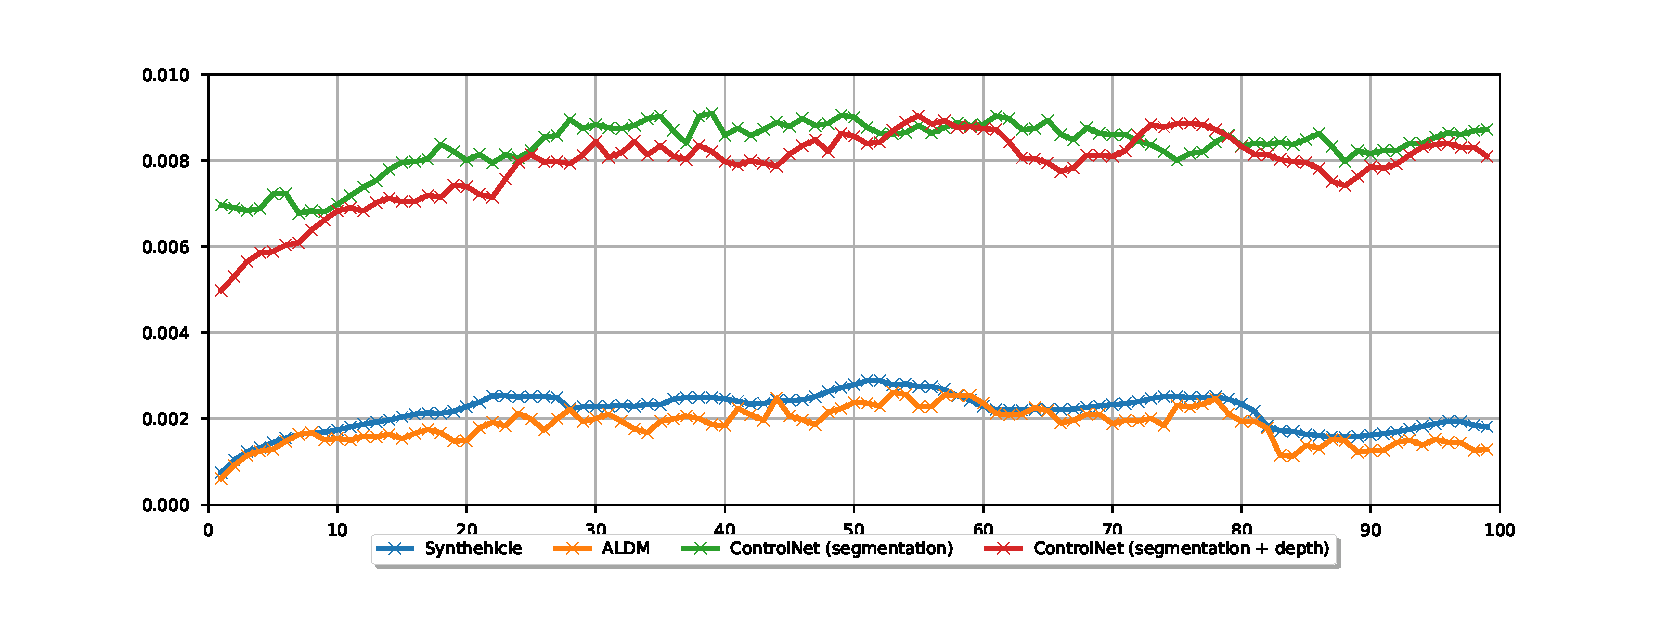
\includegraphics[width=\textwidth]{figures/evaluation/plot_rmse.pdf}
  \caption{RMSE between two following frames. Nearer to the Sythehicle baseline video means better consistency between two frames.}
  \label{fig:rmse_video}
  \clearpage
\end{figure}

\begin{table}[H]
\centering
\small
    \begin{tabular}{lLLLLRL}
    \toprule
          
    Video & \text{Syntheticle} & \text{ALDM} & \text{I2I ControlNet (seg)} &  \multicolumn{2}{c}{I2I ControlNet (seg + depth)}  \\
    \midrule
    Scene 1 & 7     & \textbf{18}   & 36    & 24            \\
    Scene 2 & 15    & \textbf{20}   & 29    & 22            \\
    Scene 3 & 2     & \textbf{4}    & 14    & \textbf{4}    \\
    Scene 4 & 8     & \textbf{8}    & 23    & 24            \\
    Scene 5 & 8     & \textbf{7}    & 63    & 13            \\
    Scene 6 & 9     & 15            & -     & \textbf{14}   \\
        \midrule
    Avg     & 8.2  & \textbf{12.0}  & -      & 16.8   \\
    Avg -1  & 8.2  & \textbf{10.2}  & 29     & 14   \\
    \bottomrule
    \end{tabular}%
    \caption{Results of object detection tests running on the six scenes. The original video marks the baseline. Avg -1 describes the average of all results, but the baseline score replaces the worst score of a generation method.}
    \label{tab:results_object_tracking}  
\end{table}%

\subsubsection{ALDM}
As the test results show, using ALDM for generation yields results that are nearly equivalent to the original video in terms of image stability as well as in the object detection tests. As depicted in \autoref{fig:rmse_video}, the ALDM model dominates the other approaches regarding RMSE between the following frames, showing how stable the images are. Compared to the original video, the RMSE is almost equal. Looking through the videos, spatial consistency is broken at two things: lightning and cars. Especially the cars, the only moving element in the videos, cannot persist in color or shape, even when the same seed is used. This comes with no surprise because of the change in the segmentation map; different pixels are now denoised to generate the cars, leading to other cars. Also, this approach lacks information from the previous frames, making feature-sharing impossible. This also partially explains the gap between the baseline video from Synthehicle and ALDM in the object detection results \autoref{tab:results_object_tracking}. Another problem with ALDM discussed earlier as well, is its training on first-person view data, making it extra hard for the model to generate realistic shapes for the cars from a third-person perspective.

For special constancy, the videos generated by ALDM follow the underlying segmentations and, therefore, are fully consistent with the ground truth.

\begin{figure}[H]
  \centering
  \includegraphics[width=\textwidth]{figures/evaluation/video_analysis.pdf}
  \caption{Frames 21-24 of Scene 1. From top row to bottom row:
synthetic data from Synthehicle, Output ALDM, Output I2I Seg, Output I2I Seg + Depth. The red boxes mark where a pedestrian can be seen clearly.}
  \label{fig:video_analysis}
  \clearpage
\end{figure}

\subsubsection{Image-to-Image with the Segmentation ControlNet}
Looking at the RMSE, image-to-image with a segmentation ControlNet overall performs the worst out of all tested approaches. The information from the previous image combined with the segmentation is too little information to obtain a consistent background, resulting in new generations in each frame.

This is especially bad for the car generation because, together with the prompt, objects that are distorted by previous generations are often converted to cars, resulting in really bad performance in object tracking.

\subsubsection{Image-to-Image with the Depth and Segmentation ControlNet}
For the depth images, it is important to notice how much better details are captured during generation. Looking at the person in Scene 1 \autoref{fig:video_analysis}, in contrast to generation only with the segmentation map, the person is visible and moving correctly. 

This behavior is also captured by the object tracking test. While the depth map does not help that much with maintaining a stable image (see \autoref{fig:rmse_video}), the performance for car tracking drastically improves over the ControlNet with segmentation, sometimes getting even closer to the original Syntehicle video than ALDM.


\subsection{Discussion: Spatial-temporal image consistency}
ALDM dominates in this area with its capabilities to maintain a very good spatial and temporal consistency, while the image-to-image approaches fall short of expectations. Particularly noteworthy here is the preservation of the background, which is almost identical to the previous image. However, it is important to note that all these attempts are based on still cameras. This means that the same noise remains in the same place, which makes it much easier to keep the background stable. With a static camera, it should also be possible to transfer the properties of the moving objects to the subsequent frames with relatively little effort and thus make the cars consistent. With a moving camera, ALDM would have to be fundamentally modified. An example of how this could work would be the \href{https://huggingface.co/CiaraRowles/TemporalNet}{TemporalNet}, which can generate the subsequent frame for another frame by being trained on time series data. Even if the presented results have strong artifacts, TemporalNet's outputs are much more stable than Stable Diffusion outputs. Another possibility would be to go the way of OpenAI Sora  \cite{liu2024sorareviewbackgroundtechnology}, which trains its entire model on time series and outputs its result at once and not iteratively. The problem with Sora's approach is the high training cost, long training time, and low data availability.  
% Conlusion and outlook
\chapter{Conclusion and Outlook}
\label{ch:conclusion}
\section{Conclusion}
In conclusion, this thesis introduced a user-friendly pipeline that integrates an intuitive interface with Stable Diffusion and evaluation frameworks, enabling the assessment of current advancements in Stable Diffusion algorithms. With its different modules, it currently allows large pipelines to generate different datasets used for evaluation. The created datasets are COCO annotated regarding their bounding boxes, with segmentation labeling and depth information available. All of these datasets are available for download and testing. 

The findings from the conducted tests suggest that while ALDM and the associated post-processing algorithms have potential, they are not yet accurate enough to fully replace synthetic data. A key challenge lies in the distortion of generated objects, particularly in their proportions, which remains problematic even after depth information is applied during post-processing.

The experiments underline the importance of training, with MUAD showing superior Average Precision (AP) and Average Recall (AR) scores compared to Synthehicle, likely due to ALDM's training on the Cityscapes dataset. An additional insight is that depth information combined with segmentation enhances the quality of a previously generated image and, therefore, consistently outperforms segmentation-only approaches. This suggests that modifying ALDM to accept both segmentation and depth information as inputs could significantly optimize the image quality.

Looking at the other tests, ALDM demonstrates strong temporal and spatial consistency, maintaining stable backgrounds and object continuity across frames, especially with stationary cameras. However, distorted car contours remain unresolved, indicating a need for further refinement.

\section{Future Work}
As shown in the conclusion, there are still a lot of topics that have to be investigated further. The future work topics can be split into two categories: the programming and the evaluation. 

\subsection{Programming Part}
The current pipeline supports most of the features used in the evaluation part, especially on the generational part. However, some metrics, especially the spatial-temporal image consistency parts, only exist as code fragments that can be adapted into modules. Overall, in the current space of LDMs, there is so much going on, leading to new technical findings that could also be adapted into more modules.

Also, user experience is currently limited. Configuration must be done in code, and the functional programming style is intuitive for computer science students but probably not for most others. A user interface a la \href{https://github.com/comfyanonymous/ComfyUI}{ComfyUI} would be a good thesis topic, especially addressing the security problems mentioned above. Also, performance is a significant point, especially parallelism, which could be used with enough computing power.

Moving away from my pipeline, enhancing ALDM could be another interesting topic. As mentioned above, expanding it with the input of depth maps or making it possible to infer information from previously generated images could be really interesting, resulting probably in results close to or even succeeding pure synthetic data.

\subsection{Evaluation Part}

While the current evaluation methods and settings are chosen by carefully analyzing different smaller samples, there are so many configuration options that it is not practical to explore all possible combinations. More tests can be quickly adapted to the existing pipelines, potentially yielding different results from those presented here. One option could be to use Stable Diffusion XL \cite{podell2023sdxlimprovinglatentdiffusion} instead of Stable Diffusion 1.5, which is often regarded as a superior diffusion model. \href{https://huggingface.co/docs/diffusers/v0.20.0/en/api/pipelines/controlnet_sdxl}{New ControlNets} have been released recently, enabling their integration into the pipeline as the image-to-image base. Additionally, training custom models could significantly improve some models' performance and is worth exploring, especially for the ALDM module, but also for addressing the temporal-spatial consistency problem discussed above.

Furthermore, other evaluation methods could be employed, particularly those with a greater focus on the image quality of the outputs from the different models. Examples of metrics could be taken from \autoref{ch:exploring_generative_ai_for_sim2real_in_driving_data_synthesis}.

%%%%%%%%%%%%%%
% Backmatter %
%%%%%%%%%%%%%%
\cleardoublepage
%\begin{appendix}
%\chapter{Upper Bounds on the Expected Error Probability}
\label{ch:appendix}

\section{Recognition Accuracy Rate}



%\end{appendix}
%\backmatter % Here, because appendix has still the mainmatter formatting

% Writes only, e.g., "bibliography" on top of those sections
\renewcommand{\chaptermark}[1]{\markboth{#1}{}}
\renewcommand{\sectionmark}[1]{\markright{#1}{}}

  
\cleardoublepage
\addcontentsline{toc}{chapter}{References}
\bibliographystyle{alpha} % Bibliography
% Add your works that are not cited in the text with the \nocite* command


\bibliography{bibliography/thesis}

\end{document}
